\documentclass[11pt,a4paper]{article}
%DIF LATEXDIFF DIFFERENCE FILE
%DIF DEL /Users/giulio/Claude/NE TNs and Blogs/TN0484/build/.latex-redline-ledhiybw/old.tex   Fri Oct 30 17:03:38 2026
%DIF ADD /Users/giulio/Claude/NE TNs and Blogs/TN0484/build/.latex-redline-ledhiybw/new.tex   Fri Oct 30 17:03:38 2026
\usepackage[margin=2.3cm]{geometry}
\usepackage{lmodern}        % classic Computer Modern look, vectorized (T1)
\usepackage[T1]{fontenc}
\usepackage{amsmath,amssymb}
\usepackage{graphicx}
\graphicspath{{figures/}}
\usepackage{xcolor}
\usepackage{booktabs}
\usepackage{longtable}
\usepackage{array}
\usepackage{fancyhdr}
\setlength{\headheight}{14pt}   % silence fancyhdr's headheight warning
\usepackage{titlesec}
% Cross-document references for the split JNE build: the article cites
% supplementary figures and the supplement cites main-text sections and
% equations. xr-hyper (not xr) is the hyperref-compatible version and must be
% loaded BEFORE hyperref. `./build.sh all` bootstraps labels before publishing.
\usepackage{xr-hyper}
\usepackage[hidelinks]{hyperref}
\usepackage{caption}
\usepackage{enumitem}
%DIF 23a23
\usepackage{placeins} %DIF >
%DIF -------
\captionsetup{font=small,labelfont=bf}
\usepackage{parskip}

% ---------------------------------------------------------------------------
% Build switch. \jnefalse -> Neuroelectrics/BCOM Technical Note (TN0484/WP0185).
%                \jnetrue  -> Journal of Neural Engineering manuscript (default: the
%                working edition; typesetting this file in TeXShop gives the article).
% One source, two outputs: the TN keeps its branding and the full appendices;
% the JNE build strips the house furniture and uses the structured abstract.
% Never fork this file -- switch the flag.
%
% The working edition is JNE: ./build.sh defaults to it. The raw TeX default
% remains TN; choose the article without editing this file via ./build.sh jne  (which invokes pdflatex as
%   pdflatex -jobname=TN0484_jne "\def\jnebuild{}\input{<this file>}" ).
% ---------------------------------------------------------------------------
\newif\ifjne
\jnetrue
\ifdefined\tnbuild\jnefalse\fi
\ifdefined\jnebuild\jnetrue\fi

% ---------------------------------------------------------------------------
% Supplement switch. \supptrue -> build ONLY the appendices and supplementary
% figures, as a standalone companion file. Selected from the command line via
%   ./build.sh supp
% JNE counts the main article against a ~12,000-word guideline; splitting the
% additional material into a separate file shortens the narrative. Integral
% model definitions remain article appendices. The TN keeps everything in one PDF.
% ---------------------------------------------------------------------------
\newif\ifsupp
\suppfalse
\ifdefined\suppbuild\supptrue\jnetrue\fi

% Notation and compact model derivations are article appendices.
% Additional topic-organized material travels with the TN and supplement.
\newif\ifappendices
\ifsupp\appendicestrue\else\ifjne\appendicesfalse\else\appendicestrue\fi\fi

\ifjne
  \ifsupp
    \IfFileExists{TN0484_jne.aux}{\externaldocument[][nocite]{TN0484_jne}}{}
  \else
    \IfFileExists{TN0484_jne_supplement.aux}{\externaldocument[][nocite]{TN0484_jne_supplement}}{}
  \fi
\fi

\definecolor{neblue}{RGB}{10,79,140}
\definecolor{negray}{RGB}{85,85,85}
\definecolor{nered}{RGB}{179,54,31}

\ifjne
  % Plain black headings; IOP typesets its own styling at production.
  \titleformat{\section}{\large\bfseries}{\thesection}{0.6em}{}
  \titleformat{\subsection}{\normalsize\bfseries}{\thesubsection}{0.6em}{}
  \pagestyle{plain}
\else
  \titleformat{\section}{\large\bfseries\color{neblue}}{\thesection}{0.6em}{}
  \titleformat{\subsection}{\normalsize\bfseries\color{negray}}{\thesubsection}{0.6em}{}
  \pagestyle{fancy}\fancyhf{}
  \lhead{\textcolor{neblue}{\textbf{NEUROELECTRICS/BCOM}}\ \textcolor{negray}{\small Technical Note}}
  \rhead{\textcolor{negray}{\small TN0484\,/\,WP0185}}
  \lfoot{\textcolor{negray}{\scriptsize Neuroelectrics / BCOM --- Preprint}}
  \rfoot{\textcolor{negray}{\scriptsize \thepage}}
  \renewcommand{\headrulewidth}{0.8pt}
  \renewcommand{\footrulewidth}{0.4pt}
\fi

\newcommand{\Sig}{\sigma}
\newcommand{\half}{\tfrac{1}{2}}
%DIF 91c92
%DIF < \newcommand{\paperver}{0.15.0-draft24}
%DIF -------
\newcommand{\paperver}{0.15.0-draft25} %DIF >
%DIF -------
\hypersetup{
  pdftitle={The cortical column as a tuned receiver: a network mechanism for temporal-interference stimulation},
  pdfauthor={Giulio Ruffini, Ricardo Salvador, Borja Mercadal, Raul de Palma Aristides, Francesca Castaldo, Nir Grossman, Santiago Canals, Claudio Mirasso},
%DIF 95c96
%DIF <   pdfsubject={TN0484 / WP0185, version \paperver, October 25, 2026}
%DIF -------
  pdfsubject={TN0484 / WP0185, version \paperver, October 30, 2026} %DIF >
%DIF -------
}
%DIF PREAMBLE EXTENSION ADDED BY LATEXDIFF
%DIF CFONT PREAMBLE %DIF PREAMBLE
\RequirePackage{color}\definecolor{RED}{rgb}{1,0,0}\definecolor{BLUE}{rgb}{0,0,1} %DIF PREAMBLE
\DeclareOldFontCommand{\sf}{\normalfont\sffamily}{\mathsf} %DIF PREAMBLE
\providecommand{\DIFaddtex}[1]{{\protect\color{blue} \sf #1}} %DIF PREAMBLE
\providecommand{\DIFdeltex}[1]{{\protect\color{red} \scriptsize #1}} %DIF PREAMBLE
%DIF SAFE PREAMBLE %DIF PREAMBLE
\providecommand{\DIFaddbegin}{} %DIF PREAMBLE
\providecommand{\DIFaddend}{} %DIF PREAMBLE
\providecommand{\DIFdelbegin}{} %DIF PREAMBLE
\providecommand{\DIFdelend}{} %DIF PREAMBLE
\providecommand{\DIFmodbegin}{} %DIF PREAMBLE
\providecommand{\DIFmodend}{} %DIF PREAMBLE
%DIF FLOATSAFE PREAMBLE %DIF PREAMBLE
\providecommand{\DIFaddFL}[1]{\DIFadd{#1}} %DIF PREAMBLE
\providecommand{\DIFdelFL}[1]{\DIFdel{#1}} %DIF PREAMBLE
\providecommand{\DIFaddbeginFL}{} %DIF PREAMBLE
\providecommand{\DIFaddendFL}{} %DIF PREAMBLE
\providecommand{\DIFdelbeginFL}{} %DIF PREAMBLE
\providecommand{\DIFdelendFL}{} %DIF PREAMBLE
%DIF HYPERREF PREAMBLE %DIF PREAMBLE
\providecommand{\DIFadd}[1]{\texorpdfstring{\DIFaddtex{#1}}{#1}} %DIF PREAMBLE
\providecommand{\DIFdel}[1]{\texorpdfstring{\DIFdeltex{#1}}{}} %DIF PREAMBLE
%DIF COLORLISTINGS PREAMBLE %DIF PREAMBLE
\RequirePackage{listings} %DIF PREAMBLE
\RequirePackage{color} %DIF PREAMBLE
\lstdefinelanguage{DIFcode}{ %DIF PREAMBLE
%DIF DIFCODE_CFONT %DIF PREAMBLE
  moredelim=[il][\color{red}\scriptsize]{\%DIF\ <\ }, %DIF PREAMBLE
  moredelim=[il][\color{blue}\sffamily]{\%DIF\ >\ } %DIF PREAMBLE
} %DIF PREAMBLE
\lstdefinestyle{DIFverbatimstyle}{ %DIF PREAMBLE
	language=DIFcode, %DIF PREAMBLE
	basicstyle=\ttfamily, %DIF PREAMBLE
	columns=fullflexible, %DIF PREAMBLE
	keepspaces=true %DIF PREAMBLE
} %DIF PREAMBLE
\lstnewenvironment{DIFverbatim}{\lstset{style=DIFverbatimstyle}}{} %DIF PREAMBLE
\lstnewenvironment{DIFverbatim*}{\lstset{style=DIFverbatimstyle,showspaces=true}}{} %DIF PREAMBLE
%DIF END PREAMBLE EXTENSION ADDED BY LATEXDIFF

\begin{document}
\emergencystretch=3em
\noindent{\small Changes relative to v0.15.0-draft24 (8ecc70a).}\par

\ifjne
% ---------------------------------------------------------------------------
% TODO before submission: confirm affiliations 3 and 4 with Canals and Mirasso
% (reconstructed from the Overleaf edit plus the Zenodo deposit, not yet checked
% by them); confirm corresponding-author email. ORCIDs below verified against
% the ORCID registry (2026-07-21).
% Alex Just removed from the author list per Giulio, 2026-10-21 (no contribution to date).
% Ricardo Salvador's ORCID supplied as registry-verified by giulio-shell on
% 2026-10-09. Giulio confirmed Ricardo as second author on 2026-10-21.
% ---------------------------------------------------------------------------
\begin{center}
{\LARGE\bfseries The cortical column as a tuned receiver:\\[4pt]
a network mechanism for temporal-interference stimulation}\\[16pt]
{\large Giulio Ruffini$^{1,2}$, Ricardo Salvador$^{1}$, Borja Mercadal$^{1}$,\\[2pt]
Raul de Palma Aristides$^{2}$, Francesca Castaldo$^{1,2}$,\\[2pt]
Nir Grossman$^{5}$, Santiago Canals$^{2,4}$, and Claudio Mirasso$^{2,3}$}\\[12pt]
\begin{minipage}{0.86\textwidth}\centering\small
$^{1}$Neuroelectrics, Barcelona, Spain\\
$^{2}$BCOM, Barcelona, Spain\\
$^{3}$IFISC (UIB-CSIC), Palma de Mallorca, Spain\\
$^{4}$Instituto de Neurociencias (UMH-CSIC), Sant Joan d'Alacant, Spain\\
$^{5}$Department of Brain Sciences and UK Dementia Research Institute,\\
Imperial College London, London, United Kingdom\\[6pt]
E-mail: \texttt{giulio.ruffini@neuroelectrics.com}\\[4pt]
Working draft v\paperver\quad \DIFdelbegin \DIFdel{2026-10-25
}\DIFdelend \DIFaddbegin \DIFadd{2026-10-30
}\DIFaddend \end{minipage}\\[8pt]
\begin{minipage}{0.86\textwidth}\centering\footnotesize\color{negray}
\textbf{ORCID iDs:}\ %
G.~Ruffini \href{https://orcid.org/0000-0003-3084-0177}{0000-0003-3084-0177};\ %
R.~Salvador \href{https://orcid.org/0000-0003-1235-6533}{0000-0003-1235-6533};\ %
B.~Mercadal \href{https://orcid.org/0000-0002-0941-6796}{0000-0002-0941-6796};\ %
R.~de Palma Aristides \href{https://orcid.org/0000-0002-0255-2293}{0000-0002-0255-2293};\ %
F.~Castaldo \href{https://orcid.org/0000-0002-4947-4552}{0000-0002-4947-4552};\ %
N.~Grossman \href{https://orcid.org/0000-0003-2002-9049}{0000-0003-2002-9049};\ %
S.~Canals \href{https://orcid.org/0000-0003-2175-8139}{0000-0003-2175-8139};\ %
C.~Mirasso \href{https://orcid.org/0000-0003-2980-7038}{0000-0003-2980-7038}.
\end{minipage}
\end{center}
\vspace{6pt}
\else
\begin{flushleft}
{\color{neblue}\rule{\textwidth}{2pt}}\\[4pt]
{\LARGE\bfseries The cortical column as a tuned receiver:\\[2pt]
a network mechanism for temporal-interference stimulation}\\[10pt]
\begin{tabular}{@{}ll@{}}
\textbf{Document:} & TN0484 (Neuroelectrics TN)\,/\,WP0185 (BCOM WP) \\
\textbf{Authors:} & Giulio Ruffini, Ricardo Salvador, Borja Mercadal,\\
& Raul de Palma Aristides, Francesca Castaldo,\\
& Nir Grossman, Santiago Canals, and Claudio Mirasso \\
\textbf{Affiliations:} & Neuroelectrics\,/\,BCOM\,/\,IFISC (UIB-CSIC)\,/\,IN (UMH-CSIC)\\
& Imperial College London (Brain Sciences and UK Dementia Research Institute) \\
\textbf{Date:} & \DIFdelbegin \DIFdel{2026-10-24 }\DIFdelend \DIFaddbegin \DIFadd{2026-10-30 }\DIFaddend \qquad \textbf{Version:} \paperver \\
\textbf{DOI:} & \href{https://doi.org/10.5281/zenodo.21009618}{10.5281/zenodo.21009618} \\
\end{tabular}\\[4pt]
{\color{neblue}\rule{\textwidth}{1pt}}
\end{flushleft}
\fi

\ifsupp
\begin{center}
{\large\bfseries Supplementary Material}\\[4pt]
\begin{minipage}{0.86\textwidth}\centering\small
Additional methods, derivations, and figures accompanying the article. Sections, equations, and figures use S-prefixed numbers;
references to article equations are marked as main-text references.
\end{minipage}
\end{center}
\vspace{8pt}
\fi

\ifsupp\else
\section*{Abstract}
% One text for the article, technical note, and storyline.

\noindent
\ifjne
\textbf{Objective.} We develop a mesoscale model of temporal-interference (TI) stimulation with three stages
in series: membrane access, nonlinear detection of the difference frequency absent from
the field, and circuit amplification.\
\textbf{Approach.} We represent access by an effective membrane time and analyze detection and
amplification in a Jansen--Rit column, an exact mean field of quadratic
integrate-and-fire (QIF) neurons, and its spiking network. We compare spatial maps in
one head model and quantify conditional kHz access budgets.\
\textbf{Main results.} For weak fields, a static quadratic detector generates a beat proportional to the
carrier-polarization product and a signed, direct-current-like (DC-like) steady source
proportional to their summed squares. Transcranial alternating-current (tACS) and direct-current (tDCS)
stimulation sources are linear to leading order. At the pinned
Jansen--Rit operating point, 0.1--0.3 mV per carrier gives TI sources approximately
2--5\% of direct sources at equal per-carrier and direct-input
polarizations. Dynamic QIF detection crosses from static curvature to positive-slope
rectification at fast carriers. Changing the current ratio moves the hippocampal
envelope and mean-square centroids oppositely but only rescales the beat map at
fixed state. Near a Hopf bifurcation, resonant gain grows inversely with modal damping
and is shared with tACS. In the pinned Jansen--Rit column, coupling changes gain
independently of detection; amplification appears mainly in beat-locked population-rate
modulation, with little mean-rate change. At stronger inputs, the steady source alone drives the circuit across its gamma
threshold, as does an unmodulated carrier matched in root-mean-square (RMS) input.\
\textbf{Significance.} Weak-field beat dose follows the polarization product rather than the envelope minimum.
The steady source can act at depth; its sign depends on detector state and dynamics,
not carrier polarity. For uniform scalar coupling and detection in homogeneous
conductivity, its magnitude has no strict interior maximum. Polarization measurements and amplitude and frequency sweeps test the
stages; physiological kHz coupling remains uncalibrated.
\else
We develop a mesoscale model of temporal-interference (TI) stimulation with three stages
in series: membrane access, nonlinear detection of the difference frequency absent from
the field, and circuit amplification.\ We represent access by an effective membrane time and analyze detection and
amplification in a Jansen--Rit column, an exact mean field of quadratic
integrate-and-fire (QIF) neurons, and its spiking network. We compare spatial maps in
one head model and quantify conditional kHz access budgets.\ For weak fields, a static quadratic detector generates a beat proportional to the
carrier-polarization product and a signed, direct-current-like (DC-like) steady source
proportional to their summed squares. Transcranial alternating-current (tACS) and direct-current (tDCS)
stimulation sources are linear to leading order. At the pinned
Jansen--Rit operating point, 0.1--0.3 mV per carrier gives TI sources approximately
2--5\% of direct sources at equal per-carrier and direct-input
polarizations. Dynamic QIF detection crosses from static curvature to positive-slope
rectification at fast carriers. Changing the current ratio moves the hippocampal
envelope and mean-square centroids oppositely but only rescales the beat map at
fixed state. Near a Hopf bifurcation, resonant gain grows inversely with modal damping
and is shared with tACS. In the pinned Jansen--Rit column, coupling changes gain
independently of detection; amplification appears mainly in beat-locked population-rate
modulation, with little mean-rate change. At stronger inputs, the steady source alone drives the circuit across its gamma
threshold, as does an unmodulated carrier matched in root-mean-square (RMS) input.\ Weak-field beat dose follows the polarization product rather than the envelope minimum.
The steady source can act at depth; its sign depends on detector state and dynamics,
not carrier polarity. For uniform scalar coupling and detection in homogeneous
conductivity, its magnitude has no strict interior maximum. Polarization measurements and amplitude and frequency sweeps test the
stages; physiological kHz coupling remains uncalibrated.
\fi

\smallskip
\noindent\textbf{Keywords:} temporal interference; non-invasive neuromodulation;
transcranial stimulation; neural mass model; amplitude demodulation; Hopf bifurcation;
cross-frequency coupling; criticality.

% Kept in both builds: reviewers use the contents list to navigate.
\clearpage
\tableofcontents
\clearpage

\section{Introduction}
Temporal-interference (TI) stimulation \DIFdelbegin \DIFdel{was proposed }\DIFdelend \DIFaddbegin \DIFadd{aims }\DIFaddend to reach deep brain targets while
reducing stimulation of surrounding tissue \cite{grossman2017}. \DIFdelbegin \DIFdel{It applies two }\DIFdelend \DIFaddbegin \DIFadd{Two }\DIFaddend sinusoids at
$f_1$ and $f_2=f_1+\Delta f$ \DIFaddbegin \DIFadd{applied }\DIFaddend through separate electrode pairs, typically with
$f_1\sim1$--$2$~kHz and $\Delta f\sim1$--$100$~Hz\DIFdelbegin \DIFdel{. Where the fields overlap, their
superposition is }\DIFdelend \DIFaddbegin \DIFadd{, produce }\DIFaddend an amplitude-modulated
(AM) signal \DIFdelbegin \DIFdel{with an envelope at $\Delta f$. Electrode currents can steer }\DIFdelend \DIFaddbegin \DIFadd{where their fields overlap. Changing the currents steers }\DIFaddend the region
of largest envelope modulation. \DIFdelbegin \DIFdel{Whether this
also localizes the neural response }\DIFdelend \DIFaddbegin \DIFadd{Neural targeting also }\DIFaddend depends on how neurons
transduce \DIFdelbegin \DIFdel{the }\DIFdelend \DIFaddbegin \DIFadd{this }\DIFaddend waveform.

The difference frequency is absent from the input itself:
\begin{equation}
s(t)=\varepsilon_1\cos(\omega_1 t)+\varepsilon_2\cos(\omega_2 t),\qquad
\omega_{1,2}=2\pi f_{1,2},\quad \Omega=\omega_2-\omega_1=2\pi\,\Delta f .
\label{eq:am}
\end{equation}
Here $s(t)$ is the local membrane polarization, $t$ is time, and
$\varepsilon_{1,2}$ are its tone amplitudes in mV, produced by coupling of the applied field to the membrane; $\Omega$ is the beat angular frequency, and
$f_c=(f_1+f_2)/2$ is the carrier frequency. The spectrum contains only the two applied lines. A linear, time-invariant system can attenuate or phase-shift
them but cannot create a new one. Passive membrane filtering therefore cannot
demodulate TI \cite{mirzakhalili2020}; a nonlinear element must mix the carriers into
the low-frequency band, as in AM reception \cite{nahin2001}.

The mechanism has three \DIFdelbegin \DIFdel{physical requirements. \emph{Access} is the conversion of the }\DIFdelend \DIFaddbegin \DIFadd{stages. \emph{Access} converts the }\DIFaddend extracellular field
into local membrane polarization. \emph{Detection}, or demodulation, \DIFdelbegin \DIFdel{is the nonlinear generation of the
difference-frequency component from those
polarizations }\DIFdelend \DIFaddbegin \DIFadd{mixes those
polarizations to generate the difference frequency}\DIFaddend . \emph{Amplification} is the
\DIFdelbegin \DIFdel{response of the neuronand its recurrent circuitto the generated component}\DIFdelend \DIFaddbegin \DIFadd{neuron's and recurrent circuit's response to that source}\DIFaddend . Strong coupling,
effective mixing, and resonant gain are distinct properties, even when \DIFdelbegin \DIFdel{cellular structures contribute }\DIFdelend \DIFaddbegin \DIFadd{the
same cellular structure contributes }\DIFaddend to several stages.

Somatic charging attenuates kHz fields, with the response also depending on cable
geometry and field coupling \cite{deitcher2017,eyal2016}. Esmaeilpour et al.\
\cite{esmaeilpour2021} already modeled TI sensitivity using a short, axon-like
membrane time, distinguishing sensitivity from selectivity mediated by
network adaptation. Cohen et al.'s conducting periaxonal space separates nodal and
internodal voltage dynamics and supports saltatory conduction
\cite{cohen2020periaxonal}; nodes and the sodium-channel-rich axon initial segment
(AIS) are candidate access sites \cite{kole2008ais}. We represent this route by a
short effective membrane time, whose field-to-polarization transfer requires
calibration.

Detection requires that this polarization encounter a nonlinearity. Mirzakhalili
et al.\ \cite{mirzakhalili2020} demonstrated subthreshold nodal mixing in a modified
McIntyre--\allowbreak Richardson--\allowbreak Grill (MRG) myelinated-axon model
with Hodgkin--Huxley ion-channel dynamics. Cortical-neuron models also
show axonal excitation and conduction block under stronger fields \cite{wang2023}.
Luff et al.\ \cite{luff2024mixer} directly observed subthreshold difference-frequency
oscillations in individual neurons, including carriers near $5$~kHz. Mixing persisted
during synaptic blockade but was suppressed by blocking tetrodotoxin-sensitive sodium
channels. This establishes cellular detection without locating its compartment. Smooth
cellular responses admit a population-level second-order expansion; a static
rate curve supplies it through curvature.

Amplification determines whether the generated beat appreciably changes activity.
Intrinsic currents, including the hyperpolarization-activated current $I_h$ and
M-type potassium current $I_M$, can tune a single neuron \cite{hutcheonyarom2000},
as in the cell- and state-dependent hippocampal TI responses of de Palma Aristides
et al.\ \cite{depalma2026ti}. Recurrent excitatory--inhibitory circuits supply another
resonance \cite{brunelhakim1999,brunelwang2003,ledoux2011}. In slices, pyramidal and
parvalbumin (PV) neurons respond differently, and most pyramidal TI responses
vanish under synaptic blockade \cite{caldas2024}; simulations also find network
mediation \cite{karimi2024,esmaeilpour2021}. Reviews summarize these mechanisms
\cite{soroushi2025,wangw2026}. At human-comparable fields, primate recordings show
weaker effects than direct low-frequency stimulation, expressed mainly in spike
timing rather than mean rate \cite{vieira2024}.

We focus on weak stimulation-induced changes around ongoing activity, which may
already include spiking. Direct carrier-evoked spiking and conduction block
\cite{opancar2025,peripheral2023,semenov2025} lie outside this expansion; the
finite-amplitude network examples are identified separately.

The framework \DIFdelbegin \DIFdel{in }\DIFdelend \DIFaddbegin \DIFadd{of }\DIFaddend Fig.~\ref{fig:concept} combines cellular mixing with recurrent gain, extending
models of endogenous cross-frequency coupling
\cite{ruffini2025cfc,ruffini2025ham}. Cassar\`a et al.\ already identified the
fixed-pattern consequence of second-order mixing \cite{cassara2025part2}.
Here we derive steady and beat sources together, separate detector curvature
from recurrent gain at a pinned Jansen--Rit (JR) operating point, and derive
the static-to-dynamic crossover in an exact QIF mean field. A head-model
illustration compares the resulting spatial maps, while equal-RMS carrier
controls distinguish beat-dependent modulation from induced oscillations.
\DIFdelbegin \DIFdel{These results specify a mechanism and its conditional input budget ; }\DIFdelend \DIFaddbegin \DIFadd{The resulting input budget is conditional on }\DIFaddend the field-to-detector transfer\DIFaddbegin \DIFadd{,
which remains uncalibrated }\DIFaddend at physiological kHz fields\DIFdelbegin \DIFdel{remains uncalibrated}\DIFdelend .

\begin{figure}[t!]
\centering
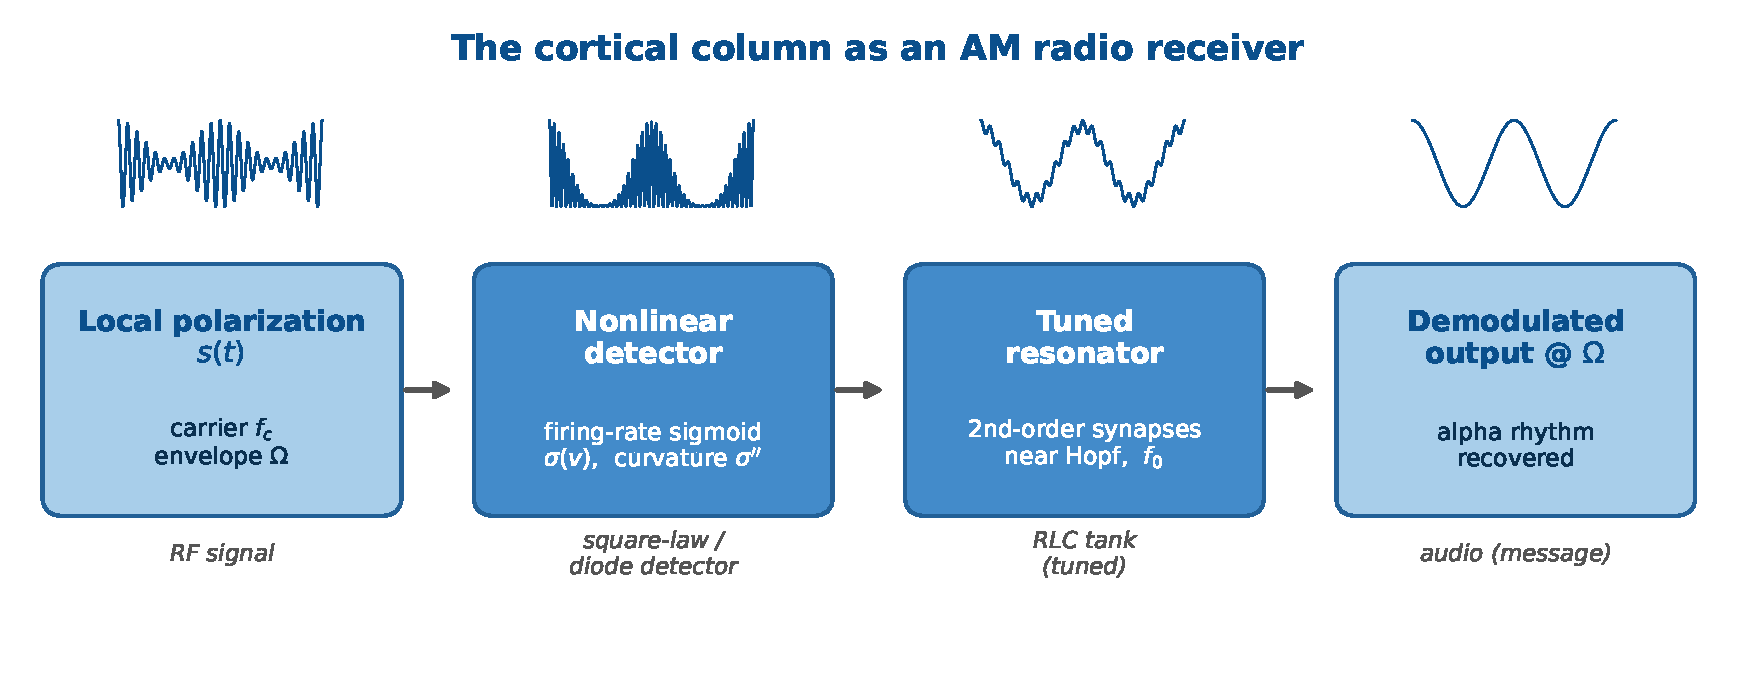
\includegraphics[width=\textwidth]{fig_concept.pdf}
%\vspace{-2cm}

\caption{\textbf{The cortical column as a tuned receiver.} Access converts the
applied field into the local polarization entering the detector. The nonlinear detector
generates the beat at angular frequency $\Omega$ from a carrier near $f_c$; a
recurrent network amplifies it near its natural frequency $f_0$. The diagram shows
the static-sigmoid realization. In a conventional AM receiver, the tuned circuit
selects the carrier before detection \cite{nahin2001}; here the resonator selects
the low-frequency output. }
\label{fig:concept}
\end{figure}

\section{Theory}

\subsection{A population rate curve supplies the nonlinearity}\label{sec:nmm}
A neural mass model describes a population through averaged variables
\cite{ruffini2025rosetta,jansen1995}. In the Jansen--Rit (JR) family, a linear synaptic
filter converts presynaptic firing rate $r(t)$ into postsynaptic potential $u_{\rm PSP}(t)$:
\[
\ddot u_{\rm PSP}+2a\dot u_{\rm PSP}+a^2u_{\rm PSP}=Aa\,r(t),
\]
with inverse synaptic time $a$ (s$^{-1}$) and PSP gain $A$ (mV); inhibitory synapses use
$b$ and $B$ in the same respective units. Summed postsynaptic potentials give the mean input $v$, which
a static transfer curve converts to firing rate \cite{wilsoncowan1972},
\begin{equation}
\Sig(v)=\frac{2e_0}{1+e^{\,\rho(v_0-v)}} .
\label{eq:sigmoid}
\end{equation}
Here $2e_0$ is the maximum rate, $v_0$ the inflection voltage, and $\rho$ the inverse
voltage scale (s$^{-1}$, mV, and mV$^{-1}$, respectively). Primes denote
derivatives with respect to voltage. Nonzero curvature makes this curve a mixer, while its slope sets
the local gain of the recurrent circuit.

The JR column couples pyramidal, excitatory-interneuron, and inhibitory-interneuron
populations, with field input to the pyramidal sigmoid and local field potential
(LFP) proxy $v=y_1-y_2$, where $y_1$ and $y_2$ are the excitatory and inhibitory
postsynaptic potentials onto the pyramidal population. Its external input rate is
$p$ (s$^{-1}$), and $C$ is the dimensionless connectivity scale.

Figure~\ref{fig:models} locates the field input, nonlinear detector, and
recurrent amplifier in the JR and QIF circuits.
\begin{figure}[t!]
\centering
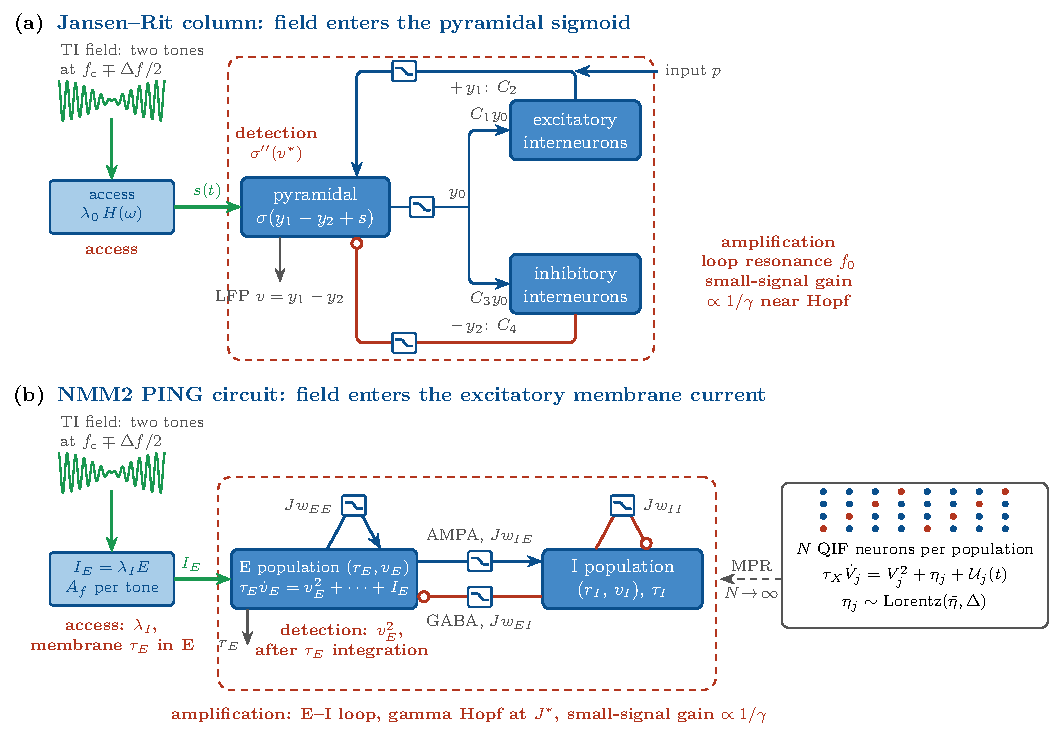
\includegraphics[width=\textwidth]{fig_models_ti.pdf}
\caption{\textbf{Access, detection, and amplification in the two circuits.}
\emph{(a)} JR: access $\lambda_0H(\omega)$ converts the field to polarization
$s$, and sigmoid curvature mixes the tones.
\emph{(b)} NMM2 PING: current $I_E=\lambda_I E$ enters the excitatory membrane;
$v_E^2$ mixes its voltage excursions. The inset shows the QIF neurons whose
infinite-population limit gives this exact mean field.
Low-pass symbols mark second-order synapses ($h_e,h_i$ in a; AMPA and GABA
with times $\tau_a,\tau_g$ in b). They suppress carriers more strongly than
the generated beat and transmit the steady shift.
Dashed frames enclose recurrent amplifiers, with small-signal gain
proportional to $1/\gamma$ near the relevant Hopf.
Blue: excitation; red: inhibition; green: field input.}
\label{fig:models}
\end{figure}


\subsection{From applied field to a squared-envelope beat component}\label{sec:coupling}
We neglect propagation and induction in the extracellular field $E(t)$ (V/m),
but retain finite membrane charging. The effective polarization $s(t)$ (mV)
enters the population sigmoid after cellular access:
\begin{equation}
r(t)=\Sig\!\big(v(t)+s(t)\big),\qquad
E(t)=E_1\cos\omega_1 t+E_2\cos\omega_2 t .
\label{eq:coupling}
\end{equation}
Soma, dendrites, AIS, nodes, and terminals contribute parallel inputs with
different couplings and response times. For nearby carriers centered at
$\omega_c=2\pi f_c$,
\begin{equation}
s(t)\simeq\sum_k \boldsymbol\lambda^k_f(\omega_c)\!\cdot\!\mathbf E(t),\qquad
\boldsymbol\lambda^k_f(\omega)=\boldsymbol\lambda^k_0\,\lvert H_k(\omega)\rvert,
\label{eq:doors}
\end{equation}
where $\boldsymbol\lambda^k_0$ is compartment $k$'s static polarization vector
(a length) and $H_k$ its access filter \cite{ruffini2025rosetta,galangadea2023}.
This amplitude-gain sum assumes aligned compartment phases; otherwise the
complex transfers must be summed. For one dominant entry point,
$\lambda_f=\lambda_0|H|$ and $\varepsilon_j=\lambda_f(\omega_j)E_j$.
Holding these post-access polarizations fixed isolates detection and gain;
at fixed field they inherit $H$'s frequency dependence.

Fast axonal access motivates $\lambda_f\approx\lambda_0$. At the AIS,
$\Sig(v+s)$ represents a spike-initiation threshold shifted from $v_0$ to
$v_0-s$, requiring no backward transmission to the soma. The conversion from
AIS polarization to $s$ and its response time require calibration. \DIFdelbegin \DIFdel{Fast
access alone does not establish a static
detector at the carrierfrequency
(\S\ref{sec:dynamic})}\DIFdelend \DIFaddbegin \DIFadd{A static
detector additionally requires relaxation faster than the carrier}\DIFaddend .

Expanding about the field-free voltage $v^*$ (mV)
\cite{ruffini2025ham} gives
$\Sig(v^*+s)\approx\Sig(v^*)+\Sig'(v^*)s+\half\Sig''(v^*)s^2+\dots$.
Quadratic mixing leads when $|s|\ll1/\rho\approx1.8$~mV and
$\Sig''(v^*)\ne0$; larger excursions require the full curve.
The linear term preserves the carriers, while
$2\cos\omega_1t\cos\omega_2t=\cos\Omega t+\cos(\omega_1+\omega_2)t$
generates their difference. Averaging over the carrier removes the fast terms
before applying network gain; synaptic filtering suppresses those terms
downstream of detection. Since $\langle\cos^2\omega_jt\rangle_c=\half$,
\begin{equation}
\big\langle\Sig(v^*+s)\big\rangle_c
=\Sig(v^*)+\tfrac14\Sig''(v^*)\,(\varepsilon_1^2+\varepsilon_2^2)
+\tfrac12\Sig''(v^*)\,\varepsilon_1\varepsilon_2\cos\Omega t+O(\varepsilon^4),
\label{eq:taylor}
\end{equation}
giving a signed beat-source amplitude
\begin{equation}
Y_\Omega\simeq\half\,\Sig''(v^*)\,\varepsilon_1\varepsilon_2 ,
\label{eq:demod}
\end{equation}
in s$^{-1}$ before recurrence, alongside the steady (DC) source.
Here $\varepsilon$ denotes a common small-amplitude scale and $\simeq$
denotes leading order in polarization throughout.

For a dynamic cellular response with synaptic input held fixed, define
the second-order coefficient $\chi^{(2)}$ through the complex source amplitude,
\begin{equation}
Y_\Omega\simeq\chi^{(2)}(\omega_2,-\omega_1)\,
\varepsilon_2\varepsilon_1,\qquad
r_\Omega(t)=\operatorname{Re}\!\left[Y_\Omega e^{i\Omega t}\right].
\label{eq:chi2}
\end{equation}
The generated rate $r_\Omega$ precedes recurrence, so $\chi^{(2)}$ has units
s$^{-1}$mV$^{-2}$. With this cosine-amplitude convention, its memoryless
limit is $\Sig''/2$. Cellular history, state, and response times can make
it complex and frequency-dependent; symmetry or cancellation can remove
second-order mixing, leaving higher orders.

The static detector predicts quadratic scaling, a vanishing source at the
inflection, and carrier independence at fixed polarization. At fixed field,
access attenuation raises the field required for a given source, consistent
with carrier-dependent thresholds \cite{opancar2025,peripheral2023}.

\subsection{Envelope oscillations and spatial weighting}\label{sec:envelope}
Envelope following and quadratic detection assign different spatial doses
to the same field. At position $\mathbf x$, let $\varepsilon_j(\mathbf x)$ be
the signed polarization of tone $j$ along a fixed direction. The nonnegative
envelope of the two-tone polarization is
\[
\mathcal A(\mathbf x,t)=\sqrt{\varepsilon_1(\mathbf x)^2+\varepsilon_2(\mathbf x)^2
+2\varepsilon_1(\mathbf x)\varepsilon_2(\mathbf x)\cos\Omega t}.
\]
At each location, carrier averaging gives
\begin{equation}
\mathrm{LPF}[s^2(t)]=\tfrac12\mathcal A^2(t)
=\frac{\varepsilon_1^2+\varepsilon_2^2}{2}+\varepsilon_1\varepsilon_2\cos\Omega t,
\label{eq:sqenv}
\end{equation}
with spatial arguments suppressed. The squared envelope is sinusoidal at
$\Omega$; the envelope itself is not. For matched tones it is the rectified
cosine $\mathcal A(t)=2\varepsilon|\cos(\Omega t/2)|$.
The conventional TI map measures its excursion,
$\mathcal M[y]\equiv\max_t y-\min_t y$ \cite{grossman2017}.

Table~\ref{tab:transduction-maps} separates these geometric quantities from
detector gains; overbars denote beat-period means. An ideal envelope follower
outputs $c_1\mathcal A$ for gain $c_1$, whereas a smooth transfer $g$ with
nonzero curvature gives $g''(v^*)\mathcal A^2/4$ at weak input ($g=\Sig$ in JR).
Thus the nonnegative mean-square map $\mathcal I$ specifies neither excitation
nor suppression, and an envelope-excursion map alone specifies no mean output.
Envelope following is itself a response assumption.

\begin{table}[ht]
\centering\small
\renewcommand{\arraystretch}{1.4}
\begin{tabular}{@{}>{\raggedright\arraybackslash}p{0.22\textwidth}
 >{\raggedright\arraybackslash}p{0.34\textwidth}
 >{\raggedright\arraybackslash}p{0.36\textwidth}@{}}
\toprule
 & Envelope following & Quadratic detection \\
\midrule
Slow signal & $\mathcal A(\mathbf x,t)$ & $\tfrac12\mathcal A(\mathbf x,t)^2$ \\
Mean before gain & $\overline{\mathcal A}(\mathbf x)$
 & $\mathcal I(\mathbf x)=\dfrac{\varepsilon_1^2+\varepsilon_2^2}{2}$ \\
Modulation excursion & $2\min(|\varepsilon_1|,|\varepsilon_2|)$
 & $2|\varepsilon_1\varepsilon_2|$ \\
Units before detector gain & mV & mV$^2$ \\
Signed steady source (output units) & $c_1\overline{\mathcal A}$
 & $Y_{\rm DC}=\tfrac12g''(v^*)\mathcal I$ \\
\bottomrule
\end{tabular}
\caption{Envelope and quadratic maps at the same position $\mathbf x$.
The first four rows give geometric quantities before detector gain; the last
gives the steady source after gain, before recurrent feedback. Its sign depends
on the detector. Averaging the slow signal over a beat period gives its mean.
Excursion means maximum minus minimum, not Fourier amplitude.}
\label{tab:transduction-maps}
\end{table}

The excursion maps in Table~\ref{tab:transduction-maps} are related pointwise by
\begin{equation}
\mathcal{M}\big[\tfrac12\mathcal A^2\big]=\max(|\varepsilon_1|,|\varepsilon_2|)\;\mathcal{M}[\mathcal A].
\label{eq:reweight}
\end{equation}
The dominant polarization reweights the envelope map. Both maps can have a
central maximum, although the quadratic example in Fig.~\ref{fig:spatial_maps}a
is broader. A larger superficial dominant carrier degrades deep contrast:
for $(\varepsilon_1,\varepsilon_2)=(10,1)$ superficially and $(0.5,0.5)$
at depth, the superficial/deep excursion ratios are $2$ for the envelope
and $40$ for the quadratic map. A sufficiently weak second carrier can
instead suppress the superficial product. Actual contrast requires the
vector fields.

With fixed electrode pairs, frequencies, neural state, linear access, and
projection directions, write
$\varepsilon_j(\mathbf x)=I_j^{\rm pair}\mathcal P_j(\mathbf x)$,
where $I_j^{\rm pair}>0$ is peak pair current (mA) and $\mathcal P_j$ is
signed polarization per current (mV/mA). Then
\[
\mathcal M[\tfrac12\mathcal A^2]
=2I_1^{\rm pair}I_2^{\rm pair}|\mathcal P_1\mathcal P_2|.
\]
Changing the ratio therefore rescales the beat map without moving its maxima
or changing normalized maps and target/reference ratios
\cite{cassara2025part2}. Fixed detector coefficients and linear propagation
preserve the common current factor, even with dynamic mixing and heterogeneous
gains. Steering requires a changed carrier field shape, for example through
current redistribution among electrodes at one frequency.

The steady map instead weights $\mathcal P_1^2$ and $\mathcal P_2^2$ by
the squared currents. Its ratio-dependent source can shift operating points
and thereby reshape the beat response. Threshold effects also depart from
the weak quadratic regime; the $2\min$ steering law requires envelope
following. The product law itself permits an interior beat maximum.
Local detector and network factors weight this product
(Eq.~\eqref{eq:receiver}); resonance can compensate for an unfavorable
product only where the source is nonzero.

The scalar maps use a common fixed projection,
$\varepsilon_j=\boldsymbol\lambda\cdot\mathbf E_j$; the beat changes phase
when either projection changes sign. More generally, let $a_j^k$ be the
complex polarization of carrier $j$ in compartment $k$. A weak dynamic
detector has a bilinear beat source
$Y_\Omega=\sum_{kl}B_{kl}(\omega_2,-\omega_1)a_2^k\overline{a_1^l}$,
where $B_{kl}$ are fixed response coefficients and the overbar means complex
conjugation. A single scalar input is a rank-one specialization. Linear
access gives $a_j^k=I_j^{\rm pair}b_j^k$, with $b_j^k$ the polarization per
unit current, so the common factor $I_1^{\rm pair}I_2^{\rm pair}$ and its
fixed spatial pattern survive without a universal projection vector.

\subsection{Detector laws and harmonic signatures}\label{sec:transduction}
For a narrowband input $s(t)=\mathcal A(t)\cos\omega_c t$, a memoryless
nonlinearity $g$ has low-frequency output given by its carrier-cycle average,
\[
Y_{\rm LF}(\mathcal A)=(2\pi)^{-1}\!\int_0^{2\pi}\!g(v^*+\mathcal A\cos\theta)\,\mathrm{d}\theta,
\]
where $\theta$ is carrier phase. This transduction contains
only even powers:
\begin{equation}
Y_{\rm LF}(\mathcal A)=g(v^*)+\tfrac14 g''(v^*)\mathcal A^2+\tfrac1{64}g^{(4)}(v^*)\mathcal A^4+\cdots
\label{eq:cycavg}
\end{equation}
Thus smooth detection with nonzero curvature is quadratic at weak input.
\DIFdelbegin \DIFdel{Other laws require different detectors: full- and half-wave rectifiers yield
$2\mathcal A/\pi$ and $\mathcal A/\pi$, a diode-and-capacitor detector follows the peak, and a step with offset $\delta>0$ yields
}\DIFdelend \DIFaddbegin \DIFadd{A threshold detector instead gives
}\DIFaddend $\pi^{-1}\arccos(\delta/\mathcal A)$ \DIFdelbegin \DIFdel{above threshold }\DIFdelend \DIFaddbegin \DIFadd{for envelope amplitude
$\mathcal A>\delta$ }\DIFaddend and zero below\DIFdelbegin \DIFdel{.
Channel rectification, threshold crossing, and release events are possible
biological implementations}\DIFdelend \DIFaddbegin \DIFadd{, where $\delta>0$ is its offset.
Other rectifier laws are compared in the supplement (\S\ref{supp:harmonics})}\DIFaddend .

At matched tones, envelope following is linear in amplitude with
second/fundamental harmonic ratio $1/5$. Quadratic detection gives only
the steady term and fundamental; its quartic correction gives
$Y_{2\Omega}/Y_\Omega\sim(c_4/c_2)\varepsilon^2$, with
$c_2=g''/4$ and $c_4=g^{(4)}/64$. A threshold detector is silent for
$2\varepsilon\le\delta$ and has an amplitude-dependent ratio above onset.
The full harmonic series and mixed-detector inversion are supplementary
(\S\ref{supp:harmonics}).
\ifjne\else
\subsection{Harmonic ladder and mixed detectors}\label{supp:harmonics}
\DIFaddbegin \DIFadd{Full- and half-wave rectifiers yield $2\mathcal A/\pi$ and
$\mathcal A/\pi$, respectively; a diode-and-capacitor detector follows the
peak. Channel rectification, threshold crossing, and release events are
possible biological implementations.
}

\DIFaddend Envelope following and square-law detection are distinguishable at a single site. At a matched target,
$\mathcal A(t)=2\varepsilon|\cos(\Omega t/2)|$, whose Fourier series
$|\cos\theta|=\tfrac2\pi+\tfrac4\pi\sum_{n\ge1}\tfrac{(-1)^{n+1}}{4n^2-1}\cos(2n\theta)$ gives a
harmonic ladder whose nonnegative Fourier amplitudes $A_{n\Omega}$ obey $A_{2\Omega}/A_\Omega=1/5$, $A_{3\Omega}/A_\Omega=3/35$ and
$A_{4\Omega}/A_\Omega=1/21$. The square-law output $\half \mathcal A^2=\varepsilon^2(1+\cos\Omega
t)$ contains only DC and $\Omega$. For the mixed family $T(\mathcal A)=c_1\mathcal A+c_2\mathcal A^2$, with
$c_1\ne0$ and a nonzero fundamental, the
pre-network ratio is
\begin{equation}
\mathcal H_{\rm det}\equiv\left|\frac{Y_{2\Omega}}{Y_\Omega}\right|
=\frac{1/5}{\left|1+\tfrac{3\pi}{4}\,c_2\varepsilon/c_1\right|},
\label{eq:rdet}
\end{equation}
so measuring $\mathcal H_{\rm det}$ constrains $c_2\varepsilon/c_1$ within this family.\footnote{The inverse has two branches unless the sign of the fundamental
relative to the linear term is known; for $c_2/c_1\ge0$ it is unique.}

\fi

The network modifies these ratios through
$\mathcal H_{\rm meas}=\mathcal H_{\rm det}|G(2\Omega)/G(\Omega)|$.
Near resonance it can suppress an envelope follower's second harmonic,
making it appear quadratic. Amplitude sweeps and gain correction are
therefore needed; one harmonic ratio cannot identify the detector.

\subsection{The steady source has a state-dependent sign}\label{sec:dc}
Detection converts nonnegative mean-square polarization into a signed steady
source; recurrence converts that source into a mean response. ``DC-like''
describes this source, not the applied field, which has no DC component.
\DIFdelbegin \DIFdel{For comparison, the envelope mean is
}\[
\DIFdel{\overline{\mathcal A}(\mathbf x)=\frac{1}{2\pi}\int_0^{2\pi}
\sqrt{\varepsilon_1(\mathbf x)^2+\varepsilon_2(\mathbf x)^2
+2\varepsilon_1(\mathbf x)\varepsilon_2(\mathbf x)\cos\vartheta}\,\mathrm d\vartheta,
}\]%DIFAUXCMD
\DIFdel{where $\vartheta$ is beat phase. }\DIFdelend At matched polarizations $\varepsilon>0$,
the envelope and quadratic means are $4\varepsilon/\pi$ and
$\varepsilon^2$ \DIFdelbegin \DIFdel{, }\DIFdelend before detector gains \DIFaddbegin \DIFadd{(supplement, \S\ref{supp:envelope-proof})}\DIFaddend . Either ideal detector gives a mean
output with one carrier, but no beat; adaptation can alter the mean response.

The static JR source is
\[
Y_{\rm DC}(\mathbf x,\mathbf n)
=\frac{\Sig''(v^*_{\mathbf x})}{2}\,\mathcal I(\mathbf x,\mathbf n),
\qquad
\mathcal I(\mathbf x,\mathbf n)
=\frac{\varepsilon_1(\mathbf x,\mathbf n)^2+
\varepsilon_2(\mathbf x,\mathbf n)^2}{2}\ge0,
\]
where $v^*_{\mathbf x}$ is the local baseline and $\mathbf n$ the common
unit cell orientation. Convex and concave rate curves give positive and
negative sources, respectively, with zero quadratic source at the inflection.
Reversing either carrier or $\mathbf n$ leaves the squares unchanged;
other orientations change magnitudes but not the sign at fixed curvature.
Figure~\ref{fig:spatial_maps}c shows both signs on one positive normalization.
At the pinned JR state, $v^*=8.30$~mV, the source lowers the local rate
because $\Sig''(v^*)<0$.
This curvature rule \DIFdelbegin \DIFdel{is static : fast-carrier QIF rectification follows a
positive slope (\S\ref{sec:dynamic}), and
recurrence further shapes the mean}\DIFdelend \DIFaddbegin \DIFadd{applies to static detection; dynamic rectification and
recurrence can change the sign of the mean response}\DIFaddend .

Carrier averaging retains the beat cross term; a beat-period average removes
it, leaving intensities without cross-frequency cancellation. Where
$Y_{\rm DC}\ne0$,
$|Y_\Omega/Y_{\rm DC}|=2|\varepsilon_1\varepsilon_2|/
(\varepsilon_1^2+\varepsilon_2^2)\le1$, with equality at matched magnitudes.
A common access factor cancels. In the preceding example, $\mathcal I$ is
$50.5$ superficially and $0.25$ at depth, a $202$-fold contrast;
the corresponding beat/DC ratios are $0.20$ and $1$.

In a homogeneous, isotropic, source-free conductor, the potentials $\phi_j$,
field components $\mathbf E_j=-\nabla\phi_j$, and polarizations
$\varepsilon_j=\boldsymbol\lambda\cdot\mathbf E_j$ for spatially fixed
coupling $\boldsymbol\lambda$ are harmonic. Consequently
$\nabla^2\mathcal I=\sum_j|\nabla\varepsilon_j|^2\ge0$:
the intensity is subharmonic, with no strict interior maximum. Its maximum
lies on the region's boundary, including conductivity interfaces, regardless
of montage. With spatially constant nonzero detection, the same holds for
$|Y_{\rm DC}|$; negative curvature makes the boundary source most negative.
Spatially varying access, orientation, or detector coefficients require a
weighted map, and the restriction does not extend to the physiological mean
response or an indefinite multicompartment DC form.

The envelope mean is also subharmonic: at each beat phase it is a norm of
harmonic components, and phase averaging preserves that property (supplement,
\S\ref{supp:envelope-proof}).
\ifjne\else
\subsection{Envelope-mean subharmonicity}\label{supp:envelope-proof}
The envelope mean \DIFdelbegin \DIFdel{has the same restriction}\DIFdelend \DIFaddbegin \DIFadd{is
}\[
\DIFadd{\overline{\mathcal A}(\mathbf x)=\frac{1}{2\pi}\int_0^{2\pi}
\sqrt{\varepsilon_1(\mathbf x)^2+\varepsilon_2(\mathbf x)^2
+2\varepsilon_1(\mathbf x)\varepsilon_2(\mathbf x)\cos\vartheta}\,\mathrm d\vartheta,
}\]
\DIFadd{where $\vartheta$ is beat phase.
}

\DIFadd{For fixed scalar coupling in homogeneous, isotropic, source-free tissue,
the envelope mean is subharmonic}\DIFaddend . At each beat phase $\vartheta$,
$\mathcal A$ is the Euclidean norm of
$(\varepsilon_1+\varepsilon_2\cos\vartheta,\,\varepsilon_2\sin\vartheta)$,
a vector of harmonic functions. A norm is convex, so this envelope is subharmonic;
averaging over $\vartheta$ preserves that property. Thus both idealized mean maps
lack a strict interior maximum under these conditions (Fig.~\ref{fig:spatial_maps}b).

\fi
By contrast,
$\nabla^2(\varepsilon_1\varepsilon_2)=2\nabla\varepsilon_1\cdot\nabla\varepsilon_2$
has unrestricted sign. Within this homogeneous scalar model, interior
selectivity must come from the oscillatory response, not either mean map.
With isotropic orientations and orientation-independent access and curvature,
orthogonal fields cancel the averaged beat while retaining steady intensity
(supplement, \S\ref{supp:orientation}).
\ifjne\else
\subsection{Isotropic orientation averages}\label{supp:orientation}
For isotropically distributed unit orientations
$\mathbf n$ with orientation-independent access and curvature,
$\langle(\mathbf n\cdot\mathbf E_j)^2\rangle=|\mathbf E_j|^2/3$
and $\langle(\mathbf n\cdot\mathbf E_1)(\mathbf n\cdot\mathbf E_2)\rangle
=\mathbf E_1\cdot\mathbf E_2/3$: orthogonal fields cancel the averaged beat,
but retain the DC intensity.

\fi
An unmodulated carrier at the same local RMS polarization gives the same
second-order mean shift if its DC mixing coefficient equals those of both
TI carriers. For a dynamic detector, that coefficient must vary negligibly
over the carrier interval.

\subsection{Comparison with direct tDCS and tACS}\label{sec:direct-comparison}
We compare TI's steady and beat sources with transcranial direct-current
stimulation (tDCS) and tACS at $\Omega$, respectively, using polarizations
at the same sigmoid entry point. For equal TI tones
$\varepsilon_1=\varepsilon_2=\varepsilon>0$,
\[
Y_{\rm DC}^{\rm TI}\simeq Y_\Omega^{\rm TI}
\simeq \frac{1}{2}\Sig''(v^*)\varepsilon^2.
\]
A constant polarization $\varepsilon_{\rm D}$ or sinusoid
$\varepsilon_{\rm A}\cos\Omega t$ instead gives
\[
Y_{\rm DC}^{\rm tDCS}\simeq\Sig'(v^*)\varepsilon_{\rm D},
\qquad
Y_\Omega^{\rm tACS}\simeq\Sig'(v^*)\varepsilon_{\rm A}.
\]
Here $\varepsilon_{\rm D}$ is signed and negative $\varepsilon_{\rm A}$
denotes phase reversal. The equivalent direct polarization matching either
TI source is
\[
\varepsilon_{\rm eq}
=\frac{\Sig''(v^*)}{2\Sig'(v^*)}\,\varepsilon^2,
\qquad
\frac{\Sig''(v^*)}{\Sig'(v^*)}
=-\rho\tanh\!\left[\frac{\rho(v^*-v_0)}{2}\right].
\]
Sigmoid steepness and operating voltage determine the ratio; the rate ceiling
cancels, and the quadratic TI sources vanish at the inflection.

For the JR parameters $\rho=0.56$~mV$^{-1}$, $v_0=6$~mV,
$e_0=2.5$~s$^{-1}$, and the pinned operating point $v^*=8.30$~mV,
$\Sig'=0.4745$~s$^{-1}$mV$^{-1}$ and
$\Sig''=-0.1508$~s$^{-1}$mV$^{-2}$. With each direct-input amplitude
equal to the per-carrier TI amplitude, the source-magnitude ratio is
$|\varepsilon_{\rm eq}|/\varepsilon
=0.1589\,\varepsilon/(1~\mathrm{mV})$:
$1.59\%$ at $0.1$~mV and $4.77\%$ at $0.3$~mV, rounded to $2$--$5\%$.
At $0.3$~mV per carrier, the equivalent direct polarization is
$-0.0143$~mV, or $-14.3~\mu$V. The negative sign specifies a suppressive
local source for tDCS and an inverted source phase for tACS.

Matching the total TI peak instead uses direct amplitude $2\varepsilon$
and halves these ratios. RMS matching uses tACS amplitude
$\sqrt2\varepsilon$ or tDCS magnitude $\varepsilon$, because TI's RMS
polarization is $\varepsilon$. The tACS quadratic steady source,
$\Sig''\varepsilon_{\rm A}^2/4$, then equals TI's for this static detector.
Equal electrode currents need not match polarization: access differs among
DC, beat and carrier frequencies, and among entry compartments.

At a common state and entry point, matched sources give matched leading
circuit responses. Steady sources share the zero-frequency transfer; beat
and tACS sources share the transfer at $\Omega$. These transfers differ,
and rectification of the amplified TI beat can add a mean shift\DIFdelbegin \DIFdel{(\S\ref{sec:timing})}\DIFdelend .
The local source comparison therefore specifies
neither a universal physiological-effect ratio nor equal spatial responses.

\subsection{Amplification: the synaptic low-pass and the network resonance}\label{sec:carrier}
Synaptic filtering suppresses the carrier after the nonlinearity has generated
the beat. Each JR excitatory synapse has transfer function
$H_s(\omega)=Aa/(i\omega+a)^2$, a second-order low-pass with characteristic
frequency $a/(2\pi)\approx16$~Hz. It passes a $10$~Hz component with relative
amplitude about $0.7$, while reducing a $100$~Hz component to about $2.5\%$. Provided the carrier does not itself excite a responsive
mode, the loop therefore reads predominantly the generated low-frequency drive.

% fig:carrier moved to Results (Theory is equations-only)

The recurrent circuit selects the recovered beat. Linearizing about the JR
fixed point gives a leading pair $\mu_\pm=-\gamma\pm i\omega_0$, with
modal damping $\gamma$ and frequency $\omega_0$. Below a supercritical
Hopf, $\gamma\to0^+$ and the quality factor
$\mathcal Q=\omega_0/(2\gamma)$ grows. A constant-numerator two-pole
approximation to the complex susceptibility $G$ gives
\begin{equation}
|G(\Omega)|\propto\big[(\omega_0^2+\gamma^2-\Omega^2)^2+(2\gamma\Omega)^2\big]^{-1/2},
\qquad |G(\omega_0)|\propto\frac{1}{2\gamma\omega_0}
\quad(\gamma\ll\omega_0),
\label{eq:gain}
\end{equation}
an approximately Lorentzian power peak near $\omega_0$ with $1/\gamma$
growth at a simple Hopf with nonzero input--output projections.\footnote{
The eigenvalue frequency $\omega_0$ differs from the canonical oscillator's
undamped frequency $\sqrt{\omega_0^2+\gamma^2}$ and peak
$\sqrt{\omega_0^2-\gamma^2}$ ($\omega_0>\gamma$).
Frequency-dependent projections can further shift the peak.}
This weak-drive law requires stability after the rectified mean shift.
Above the Hopf, entrainment instead means phase capture of an autonomous rhythm.

Write $D$ for the detector's beat-source coefficient: for the JR rate source,
$D=\half\Sig''(v^*)$, half the local sigmoid curvature. Combining access,
detection, and amplification gives
\begin{equation}
R_\Omega\simeq G(\Omega;\gamma)\;D\;\lambda_f(\omega_1)E_1\,\lambda_f(\omega_2)E_2 ,
\label{eq:receiver}
\end{equation}
% Retain the former spatial-equation label as an alias of the general receiver.
\makeatletter\begingroup\edef\@currentlabel{\theequation}\label{eq:spatial}\endgroup\makeatother
where $\lambda_f$ maps field to local carrier polarization, $D$ converts the
product of those polarizations into a beat drive, and $G$ maps that drive to the
complex observed response, whose measured amplitude is $A_\Omega=|R_\Omega|$.
For JR, $G$ is the response to a generated rate drive.
A static detector has carrier-independent $D$ at fixed polarization;
a dynamic detector can retain frequency dependence. A carrier sweep and a beat sweep
therefore constrain different stages rather than a single effective gain.

Resonance requires a beat source. The cubic Hopf normal form
responds to an in-band drive but has no second-order difference-frequency source. A large resonant susceptibility alone therefore does not
establish beat generation.

\subsection{Carrier access depends on the effective membrane response}\label{sec:khz}
Carrier independence at fixed polarization does not imply independence at fixed
applied field. As an isopotential access model, consider
$H_m(\omega)=1/(1+i\omega\tau_m)$, with effective time constant $\tau_m$.
This is the response of a point membrane to injected current; a field coupled
through a cable need not have the same transfer.
For nearby carriers, the two polarizations acquire nearly the same attenuation.
The quadratic beat then satisfies
\begin{equation}
\frac{|Y_\Omega(f_c)|}{|Y_\Omega^{\rm direct}|}
\simeq |H_m(\omega_c)|^2
=\frac{1}{1+(\omega_c\tau_m)^2}
\sim\frac{1}{(\omega_c\tau_m)^2}
\quad(\omega_c\tau_m\gg1),
\label{eq:khz}
\end{equation}
where $Y_\Omega^{\rm direct}$ is the beat generated with the same static coupling
and no access attenuation. This filter belongs either in the field-to-polarization
map or in the membrane equation that computes that polarization.

For an illustrative somatic $\tau_m=16$~ms, $|H_m|^2$ is about
$10^{-4}$, $2.5\times10^{-5}$, and $10^{-6}$ at $1$, $2$, and $10$~kHz.
The assumed $0.2$~ms case gives $0.39$ and $0.14$ at $1$ and $2$~kHz
(Fig.~\ref{fig:khz}); this transfer has not been measured under TI at an
AIS or node. Table~\ref{tab:doors} distinguishes measured responses,
assumed access, and downstream filtering. Axonal decay alone specifies
neither field coupling nor a TI cutoff.

QIF computes access in its membrane equation, requiring no additional filter
on current input. Shorter access improves transmission without determining
mixing or recurrent gain.

\begin{table}[h]
\centering\small
\renewcommand{\arraystretch}{1.15}
\begin{tabular}{@{}>{\raggedright\arraybackslash}p{2.8cm}
>{\raggedright\arraybackslash}p{3.5cm}
>{\raggedright\arraybackslash}p{8.6cm}@{}}
\toprule
Response & Time scale & Evidence and role \\
\midrule
Somatic point-membrane model & $\tau_m=16$~ms; $f_{\rm char}\approx10$~Hz &
Illustrative current-driven filter, informed by somatic measurements near $12$ and $16.5$~ms
\cite{deitcher2017,eyal2016}. \\
Myelinated axon & minimum fitted decay $\approx1$~ms &
Injected-current responses in Cohen et al.'s periaxonal circuit
\cite{cohen2020periaxonal}; evidence for distinct axonal voltage dynamics. \\
Fast axonal access & assumed $\tau_m=0.2$~ms; $f_{\rm char}\approx800$~Hz &
Reduced-model sensitivity case for a fast compartment, such as an AIS or node;
TI coupling and charging time require calibration. \\
Prior TI network model & $\tau_m=1$ and $0.4$~ms &
Short effective membrane times governing kHz sensitivity in a gamma network
\cite{esmaeilpour2021}; model parameters, not measured axonal TI decays. \\
Field-induced charging & $\approx0.7~\mu$s &
Measured with strong microsecond field pulses in isolated neurons
\cite{semenov2025}; a different stimulation regime. \\
Cellular detector & channel- and state-dependent &
Luff et al.'s TTX-sensitive mixing persists near $5$~kHz
\cite{luff2024mixer}; this measures detection, not a passive time constant. \\
JR excitatory synapse & $\tau_s=10$~ms; $f_{\rm char}\approx16$~Hz &
Model filter acting on the generated rate, downstream of detection. \\
\bottomrule
\end{tabular}
\caption{\textbf{Access, detection, and downstream filtering involve different response
times.} Measured decays, pulse-charging times, and assumed model parameters are
identified separately. The characteristic frequency $f_{\rm char}=1/(2\pi\tau)$
is given only for the specified filters; an axonal decay is not automatically a TI
cutoff. AIS, axon initial segment; TTX, tetrodotoxin.}
\label{tab:doors}
\end{table}

A sufficiently long passive cable with a sealed end in a uniform axial field
has quadratic-beat factors near $10^{-2}$ at $1$~kHz and $10^{-3}$ at
$10$~kHz for $\tau_m=16$~ms, exceeding the point-membrane values.

Any additional gate filter must represent kinetics absent from the detector
and have a model or measurement behind it. QIF lacks explicit sodium-channel
kinetics; neither it nor a static sigmoid specifies a universal $1$~kHz cutoff.
\DIFdelbegin \DIFdel{Carrier sweeps probe access and mixing together; beat sweeps probe amplification.
}\DIFdelend

\subsection{Operating-point dependence}\label{sec:opp}
\DIFdelbegin \DIFdel{Because the static source scales with $\Sig''(v^*)$, its state dependence
can be expressed through the }\DIFdelend \DIFaddbegin \DIFadd{The static JR source changes sign across the sigmoid inflection and vanishes
there and in the saturated tails. The }\DIFaddend Population Excitation--Inhibition Index
(PEIX) \cite{ruffini2025cfc} \DIFdelbegin \DIFdel{, which measures the operating point's }\DIFdelend \DIFaddbegin \DIFadd{expresses this state dependence through the }\DIFaddend signed
departure from maximal sigmoid slope\DIFdelbegin \DIFdel{:
}\begin{displaymath}
\DIFdel{\mathrm{PEIX}(v^*)=\operatorname{sign}(v^*-v_0)
\left\{1-\operatorname{sech}^2\!\Big[\tfrac{\rho}{2}\,(v^*-v_0)\Big]\right\}.
%DIFDELCMD < %%%
}\end{displaymath}%DIFAUXCMD
\DIFdel{It is zero at $v_0$ and approaches $\pm1$ in the saturated tails, with
positive sign above $v_0$. For the logistic,
$\Sig'/\Sig'(v_0)=1-|\mathrm{PEIX}|$}\DIFdelend , \DIFdelbegin \DIFdel{$\Sig'(v_0)=e_0\rho/2$, and $\Sig''=-\rho\Sig'\operatorname{sign}(\mathrm{PEIX})\sqrt{|\mathrm{PEIX}|}$. Thus this measurable state index determines the side and saturation, while
mixing follows curvature : zero at the inflection and in the tails, largest
on the flanks}\DIFdelend \DIFaddbegin \DIFadd{positive above the inflection and negative
below. Its definition and curvature identities are in Appendix~\ref{app:peix}}\DIFaddend .

Changes in $v^*$ through neuromodulation, attention, arousal, psychedelic
exposure, or dysfunction of PV interneurons in Alzheimer's disease can scale or
reverse the static JR source. Dynamic detectors have their own state-dependent
coefficients and susceptibilities, without a universal PEIX sign rule.
State sweeps therefore isolate detection only if recurrent gain is also measured.

\subsection{The exact mean field extends the static detector}\label{sec:dynamic}
The exact mean field of all-to-all quadratic integrate-and-fire (QIF) neurons
with Lorentzian excitabilities supplies both a static rate curve and its
dynamic extension. The Montbri\'o--Paz\'o--Roxin (MPR) equations evolve physical
rate $r$ and dimensionless mean voltage $v$ \cite{montbrio2015}; dynamic
synapses produce a second-generation neural mass (NMM2)
\cite{ruffini2021nmm2,clusella2023}. The population equations are
\begin{equation}
\tau_m\dot r=\frac{\Delta}{\pi\tau_m}+2rv,\qquad
\tau_m\dot v=v^2+\bar\eta-(\pi\tau_m r)^2+I(t).
\label{eq:mpr}
\end{equation}
Here $\tau_m$ is membrane time, dots denote physical-time derivatives,
$\bar\eta$ and $\Delta>0$ are the excitability center and half-width, and
$I(t)$ is dimensionless input, including recurrent drive when present.
For constant total drive $Q=\bar\eta+I$, equilibrium gives
$v=-\Delta/(2\pi\tau_m r)$ and
\begin{equation}
\tau_m r=F(Q)=\frac{1}{\pi}\sqrt{\frac{Q+\sqrt{Q^2+\Delta^2}}{2}} .
\label{eq:Fmpr}
\end{equation}
Primes on $F$ denote drive derivatives. Below its inflection at
$Q=\Delta/\sqrt3$, curvature reflects recruitment across threshold;
above it, the concave square-root rate of active cells. This nonlinearity
exists without recurrence and grows without bound, unlike the JR sigmoid.

If relaxation is faster than synaptic variation, NMM2 reduces to
$r(t)\simeq F(Q(t))/\tau_m$ with dynamically filtered recurrence
\cite{ruffini2021nmm2,clusella2023}. For population relaxation time
$\tau_{\rm rel}$ and synaptic time $\tau_s$ (Eq.~\eqref{eq:slow_synapse},
Appendix~\ref{app:models}), this requires $\tau_{\rm rel}\ll\tau_s$.
Applying the static curve to carriers further requires
$\omega_c\tau_{\rm rel}\ll1$: the same population can track synaptic
input quasistatically while responding dynamically to kHz input.
Recurrent excitatory--inhibitory circuits resonate without intrinsic
cellular resonance \cite{brunelhakim1999,brunelwang2003}. Such synaptic
modes survive the fast-membrane limit, whereas modes requiring finite
membrane dynamics need not.

Outside the adiabatic limit, the quadratic voltage term mixes the carriers
before the rate responds. For an uncoupled population under a weak current
$I_{\rm ac}\cos\omega t$, write the mean-rate shift as
$I_{\rm ac}^2\kappa_{\rm DC}/\tau_m$. At slow carriers,
$\kappa_{\rm DC}\to F''(Q)/4$; at fast carriers,
$\kappa_{\rm DC}\sim F'(Q)/[2(\omega\tau_m)^2]$.
The slow response follows curvature and can be negative above the inflection.
The fast DC coefficient instead follows the positive slope $F'$, largest at the
inflection, without a PEIX-based sign reversal: voltage excursions of order
$I_{\rm ac}/(\omega\tau_m)$ generate a positive input shift through $v^2$.
A shorter membrane time can therefore change both the magnitude and sign
of the mean response at a given physical carrier frequency.

This fast-carrier attenuation includes membrane access. Normalizing by the
squared voltage excursion leaves a coefficient tending to $F'/2$.
For two nearby current tones of amplitudes $I_j$, voltage squaring gives a
beat source proportional to $I_1I_2/(\omega_1\omega_2\tau_m^2)$.
The dynamic rate equation further attenuates the carriers after mixing;
that carrier attenuation is not applied to the generated beat. The crossover is derived in
Appendix~\ref{app:mpr-coefficients}; fixed-voltage coefficients and carrier
exponents are supplementary (\S\ref{supp:dynamic-details}).

In this cellular realization of quadratic detection, the unit coefficient of $v^2$ in membrane-time units
plays the role of $\Sig''/2$; $G$ includes the voltage and rate dynamics
converting that source into a rate beat. Other smooth cellular mechanisms
share the weak-input product law without sharing its coefficient, phase,
or carrier dependence.

\section{Methods}

\label{sec:vocab-methods}
A \emph{forced response} is the beat-driven component measured by lock-in; a purely
forced regime requires stability under stimulation. \emph{Entrainment} means
frequency and phase capture of a self-sustained oscillator \cite{pikovsky2001}.
Our frequency-dominance screen does not establish that capture. \emph{Gating}
means modulation of a persisting rhythm's amplitude \cite{canolty2010,tort2010};
a rate fold alone does not establish it. Detailed criteria are in the supplement
(\S\ref{sec:vocab}).

\subsection{Stimulation waveforms and matched-source controls}\label{sec:waveforms}
Dense perturbative sweeps use the
three-line waveform
\begin{equation}
s(t)=\varepsilon\,[\,1+m\cos\Omega t\,]\cos\omega_c t,\qquad \omega_c=2\pi f_c ,
\label{eq:amsur}
\end{equation}
with dimensionless modulation depth $m$. This AM surrogate parameterizes dense
resonance and coupling sweeps by one amplitude. It contains a central carrier
line absent from genuine TI, but matches its leading beat source:
$Y_\Omega=\half\Sig''\varepsilon^2m$. For matched genuine tones,
$\mathrm{LPF}[s^2]=\varepsilon^2(1+\cos\Omega t)$; for the $m=1$ surrogate,
$\mathrm{LPF}[s^2]=\varepsilon^2(\tfrac34+\cos\Omega t+\tfrac14\cos2\Omega t)$.
Thus the mean source differs, and the surrogate adds a second harmonic at
$25\%$ of the fundamental. We use genuine tones for the demodulation,
curvature, square-law, laminar, and kHz demonstrations, and wherever mean shifts
or harmonics enter the comparison: timing versus rate and the TI/tACS and
NMM2 endpoint controls. Open-loop agreement at the beat is checked at one
operating point; it does not imply equal driven operating states.

\subsection{Amplitude scaling and harmonic measurements}\label{sec:transduction-methods}
We sweep amplitude at fixed coupling and operating state, measuring the
fundamental and second harmonic to test the laws of \S\ref{sec:transduction}.

A software lock-in projects $v(t)$ onto sine and cosine at $\Omega$.
The finite window suppresses, but does not eliminate, neighboring frequencies.
For Hann weights $w_k$, sample times $t_k$, voltages $v_k=v(t_k)$, and
weighted mean $\bar v=\sum_k w_kv_k/\sum_k w_k$, the quadratures are
\begin{equation}
\begin{gathered}
L_{\cos}=\frac{2}{\sum_k w_k}\sum_k w_k\,(v_k-\bar v)\cos\Omega t_k,\quad
L_{\sin}=\frac{2}{\sum_k w_k}\sum_k w_k\,(v_k-\bar v)\sin\Omega t_k,\\
A_\Omega=\sqrt{L_{\cos}^2+L_{\sin}^2},
\end{gathered}
\label{eq:lockin}
\end{equation}
where $k$ indexes samples. A test tone
$v=A_{\rm test}\cos(\Omega t+\theta_0)$ with amplitude $A_{\rm test}$
and phase $\theta_0$ gives
$(L_{\cos},L_{\sin})\to A_{\rm test}(\cos\theta_0,-\sin\theta_0)$
over long windows. Thus $A_\Omega$ returns physical amplitude, twice the
Fourier-coefficient magnitude. Mean subtraction suppresses leakage from
the larger baseline (supplement, \S\ref{supp:lockin}).

\ifjne\else
\subsection{Lock-in leakage control}\label{supp:lockin}
Out-of-band components can leak into the estimate, particularly the DC level of the JR voltage readout ($\bar v\!\sim\!8$~mV, far
larger than the demodulated signal). The finite-window projection of a constant onto the quadrature references
need not vanish, so we subtract $\bar v$ explicitly; this makes the metric
accurate down to the $10^{-8}$ level needed for the JR kHz
analysis.

\fi

\DIFdelbegin \DIFdel{Measure }\DIFdelend \DIFaddbegin \DIFadd{A detector comparison requires }\DIFaddend both harmonics over the same settled window\DIFdelbegin \DIFdel{. Correct }\DIFdelend \DIFaddbegin \DIFadd{,
with }\DIFaddend their amplitude ratio \DIFdelbegin \DIFdel{by the gain ratio }\DIFdelend \DIFaddbegin \DIFadd{corrected by }\DIFaddend $|G(2\Omega)/G(\Omega)|$. The amplitude sweep tests
linear versus quadratic scaling. Estimating a mixture coefficient through
Eq.~\eqref{eq:rdet} assumes the mixed detector family and its
sign branch; a threshold detector can match one harmonic ratio.

\subsection{Head model and field computation}\label{sec:fem-methods}
\ifjne
We compute maps in IXI002, an open-access T1-weighted MRI of a 35-year-old
woman, using the hippocampal montage of Violante et al.\ \cite{violante2023}.
The six-tissue SimNIBS conductor is quasi-static with no kHz dispersion correction
\cite{salvador2025}. Pair fields are solved once and scaled to peak currents
summing to $4$~mA: $2+2$~mA for 1:1 and $1+3$~mA for 1:3. The posterior share
is swept from $0.1$ to $0.9$. Conductivities, electrodes, solver settings,
and sensitivity protocols are in the supplement (\S\ref{supp:fem-protocol}).

Local polarization is $\varepsilon_j=\lambda_0 I_j^{\rm pair}\mathbf F_j\cdot\mathbf n$
with uniform $\lambda_0=0.5$~mV per V/m \cite{radman2009} and field per unit
current $\mathbf F_j$. This coupling sets absolute amplitudes but cancels from
normalized maps, focus positions, and target-to-reference ratios. It is an
assumed field-to-polarization conversion, not a measured AIS transfer.

At each node, $\mathbf n$ maximizes the envelope at 1:1 and is then held fixed
for every ratio and every map. This geometric direction need not match a cell's
orientation. Radial and isotropically averaged orientations provide sensitivity
comparisons; the latter averages the signed beat before taking its magnitude,
allowing cancellation across orientations.

The target is the left hippocampus segmented with FreeSurfer (1,568 gray- and
white-matter nodes). The reference comprises 273,544 gray-matter nodes outside
that ROI, including other deep gray matter. The target-to-reference contrast
is the ROI 95th percentile divided by the reference 95th percentile; the
mean-based companion replaces the numerator by the ROI mean. Nodes receive
equal weight. Square roots of second-order maps provide degree-matched geometric
contrasts; the raw maps remain the detector predictions before gain.

The focus is the centroid of the top 10\% of ROI nodes ranked by each map.
Displacement is measured along the hippocampal long axis, with anterior positive.
Sensitivity checks vary montage, atlas label, gray/white-matter inclusion,
focus fraction, and orientation. These geometric maps precede detection and
recurrence: $Y_{\rm DC}=\Sig''(v^*)\mathcal I/2$ is a signed rescaling only
for uniform curvature. The head model supplies neither operating states nor
a calibrated AIS transfer.

\else
\label{supp:fem-protocol}
To compare the spatial predictions on the same anatomy, we compute all maps
in one open-access subject,
IXI002 of the IXI dataset\footnote{\url{https://brain-development.org/ixi-dataset/}}
(T1-weighted MRI; female, 35 years). The T1 image was segmented into six tissues
(scalp, skull, cerebrospinal fluid, gray matter, white matter and eyes) and meshed with
SimNIBS~3.2.3 \texttt{headreco} \cite{nielsen2018}, with its CAT12 option
\cite{gaser2024}. Tissue conductivities were 0.33 (scalp), 0.008 (skull), 1.79
(cerebrospinal fluid), 0.40 (gray matter), 0.15 (white matter) and 0.33~S/m (eyes)
\cite{salvador2025}. These are low-frequency values; no dispersion correction was
applied at the kHz carriers. The volume conductor is linear and quasi-static, so the
carrier frequencies do not enter the maps.

The electrodes follow the published hippocampal montage of Violante et al.\
\cite{violante2023}, placed by its recipe on the subject's registered 10--10
positions. Pair~1 (anterior) joins e1, 25~mm from T9 toward FT9, to e2, 10~mm from AF8
toward Fp2. Pair~2 (posterior) joins e3, 25~mm from T9 toward TP9, to e4, 10~mm from P8
toward PO8. Each electrode is a 20-mm disc of 3~mm of gel (4.0~S/m) under 2~mm of metal
(10~S/m), meshed into the head model with SimNIBS~3.2.3; the resulting mesh has
$3.64\times10^6$ linear tetrahedra. As a montage sensitivity, the 10--10 rendering of
this montage, FT7--F8 (anterior) and TP7--P8 (posterior), which Yatsuda et al.\
\cite{yatsuda2024} used as their starting montage, was meshed and solved in the same
way. Each montage has its own mesh, carrying only its own four electrodes.

Each pair was solved once at 1~A. The potential $\phi_j$ (V) satisfies
$\nabla\!\cdot\!(\sigma_{\rm cond}\nabla\phi_j)=0$, where
$\sigma_{\rm cond}$ is tissue conductivity (S/m). Current enters and leaves through each
electrode's metal contact as a Neumann condition, distributed in proportion to nodal
area; the rest of the scalp carries no normal current, and one pinned node fixes the
gauge. The linear finite-element system was assembled and solved with Neuroelectrics'
temporal-interference library, by conjugate gradients with algebraic-multigrid
preconditioning, to a relative residual of $10^{-8}$. The field
$-\nabla\phi_j$ was recovered at gray- and white-matter
nodes by superconvergent patch recovery \cite{zienkiewicz1992}, separately within each
compartment (446{,}877 node--compartment pairs). Dividing these fields by the solve
current gives the field-per-current vectors $\mathbf F_j$, expressed in
(V/m)/mA to match $I_j^{\rm pair}$. Every current condition is a scaling of these two fields.
With peak pair currents $I_1^{\rm pair}$ (anterior) and
$I_2^{\rm pair}$ (posterior) summing to 4~mA, the ratio 1:1 is $2+2$~mA and 1:3 is
1~mA anterior plus 3~mA posterior, the two conditions of Violante et al. The ratio sweep
sets the posterior share $I_2^{\rm pair}/(I_1^{\rm pair}+I_2^{\rm pair})$ from 0.1 to
0.9 in steps of 0.025.

The field-to-polarization conversion follows \S\ref{sec:envelope}:
$\varepsilon_j(\mathbf x)=I_j^{\rm pair}\mathcal P_j(\mathbf x)$, with
$\mathcal P_j=\lambda_0\,\mathbf F_j\!\cdot\!\mathbf n$, one uniform
static coupling $\lambda_0=0.5$~mV per V/m \cite{radman2009}, and
$\lambda_f\approx\lambda_0$. A uniform coupling multiplies the envelope map by
$\lambda_0$ and the two second-order maps by $\lambda_0^2$. Target-to-reference ratios,
normalized maps and focus positions do not depend on it. Hippocampal couplings of
$0.12$--$0.18$~mV per V/m \cite{bikson2004,deans2007} would scale the absolute values
by $0.24$--$0.36$ and $0.06$--$0.13$, respectively.

The detector compartment fixes the projection direction. A laminar direction for a pyramidal
axon initial segment, a local axon direction for a node, or an orientation
distribution for terminals defines a different access model. Isotropic averaging
is one possible distribution, not an anatomical consequence of choosing terminals.
Maximizing a geometric map over orientation gives an upper bound for that map
at each location; it does not identify the detector's orientation.

The projection direction $\mathbf n(\mathbf x)=\mathbf n^*(\mathbf x)$ is the envelope-maximizing direction at
the reference ratio 1:1: the closed-form maximizer, over unit vectors, of
$2\min(|\mathbf F_1\!\cdot\!\mathbf n|,|\mathbf F_2\!\cdot\!\mathbf n|)$
\cite{grossman2017}. It is chosen once at each node and then held fixed for 1:1, 1:3
and every ratio of the sweep, and all three maps use it. Along it, the 1:1 envelope map
equals its maximum over orientation. At any other ratio it is the envelope seen by an
element with that fixed orientation, which can be below that ratio's own maximum. As an
orientation sensitivity, every statistic was repeated along a second fixed field, the
radial direction from the brain centroid. The isotropic comparison averages the signed
mixing term over uniformly distributed orientations before its magnitude is taken:
$\langle\varepsilon_1\varepsilon_2\rangle_{\mathbf n}
=\lambda_0^2I_1^{\rm pair}I_2^{\rm pair}\,\mathbf F_1\!\cdot\!\mathbf F_2/3$, so the
isotropic beat excursion is
$\tfrac23\lambda_0^2I_1^{\rm pair}I_2^{\rm pair}|\mathbf F_1\!\cdot\!\mathbf F_2|$.
Elements whose beats have opposite phase cancel in this average.

The target is the left hippocampus of a FreeSurfer~6.0.0 \texttt{recon-all}
segmentation of the same T1 image (\texttt{aseg} label 17, 3903~mm$^3$)
\cite{fischl2002}. The region of interest (ROI) is the 1{,}568 gray- and white-matter
nodes inside it. The reference is the 273{,}544 gray-matter nodes outside the
ROI, including other deep gray matter. It is a gray-matter reference, not a cortex-only contrast.
The mesh and the segmentation share one image frame; tissue-volume, centroid and
white-matter checks confirmed their alignment. As a label sensitivity, the
Neuromorphometrics atlas hippocampus, warped into the subject with SimNIBS~3.2.3
\texttt{mni2subject} and the subject's nonlinear MNI transform (1{,}345 nodes; Dice 0.72
with the FreeSurfer label), replaced the ROI. As a tissue sensitivity, the ROI was
restricted to its gray-matter nodes (1{,}174 with the FreeSurfer label, 1{,}013 with
the atlas label).

The target-to-reference ratio is the ROI 95th percentile divided by the reference
95th percentile; its mean-based companion divides the ROI mean by the same
reference percentile. All percentiles and centroids weight nodes equally.
The quadratic excursion and $\mathcal I$ are second order in the field, whereas
the envelope excursion is first order. To separate this difference in degree
from the spatial weighting, each second-order statistic is also given
degree-matched, computed on the square root of the map. This is a geometric
comparison; the raw maps remain the respective detector predictions before gain.
The focus is the centroid of the top 10\% of ROI nodes,
ranked by the map's own value, with 5, 25 and 50\% as a sensitivity. Ranking makes the
focus exactly invariant to a uniform positive factor. Its displacement from 1:1 is
measured along the hippocampal long axis, the first principal axis of the ROI nodes,
with anterior positive. Field projections still use $\mathbf n^*$, independently
of this reporting axis. The 1:1 to 1:3 displacement was computed for every combination
of montage, label, ROI tissue definition and focus fraction (32 per map), each montage
along its own 1:1 direction.

No signed DC-source or mean-response map is computed. For a spatially uniform detector
coefficient, $Y_{\rm DC}=\tfrac12\Sig''(v^*)\mathcal I$ (\S\ref{sec:dc}) is
$\mathcal I$ rescaled, with the sign of $\Sig''(v^*)$. A nonuniform coefficient would
require an operating-point map, which a head model does not provide, and a mean
response would additionally require a circuit model. In particular,
$\Sig''(v^*)$ is curvature at the population model's operating point, not a
measurement of the transfer at the axon initial segment. Assigning that
coefficient to an anatomical detector requires a calibrated access and
input--output model.

\fi

\subsection{Single-column Jansen--Rit: integration, lock-in, and controls}\label{sec:jr-methods}
We integrate the JR column as six first-order ordinary differential equations. The TI field enters only the pyramidal output sigmoid, Eq.~\eqref{eq:jr0},
as $s(t)$, while the readout $v=y_1-y_2$ contains only synaptic potentials.
A beat in this readout must therefore have passed through the nonlinearity
and the recurrent loop. Unless stated otherwise $f_c=100$~Hz and $m=1$.

Integration uses fixed-step fourth-order Runge--Kutta (RK4), with time steps
chosen for each carrier band. Halving each step changes the reported lock-in
amplitudes by less than $1\%$. The resonance sweep settles for $10$~s and measures
for $20$~s; run-specific steps and windows are listed in the supplement
(\S\ref{supp:jr-runs}). The quoted $10$~kHz attenuation is analytic, not simulated.
\ifjne\else
\subsection{JR integration and measurement windows}\label{supp:jr-runs}
We integrate with a fixed-step fourth-order Runge--Kutta (RK4) scheme,
$\Delta t=2\times10^{-4}$~s (50 samples per carrier cycle at $100$~Hz; reduced to
$10^{-4}$~s for carrier sweeps up to $300$~Hz). The kHz-carrier runs of
Fig.~\ref{fig:khz_direct} use $\Delta t=2\times10^{-5}$~s for the carrier sweep to
$4$~kHz (25 samples per carrier cycle at $2$~kHz, 12.5 at $4$~kHz) and
$1.5\times10^{-5}$~s for the $2$~kHz output spectrum. Halving each step changes the
reported lock-in amplitudes by less than $1\%$. The $10$~kHz figures quoted in
\S\ref{sec:khz} are analytic evaluations of Eq.~\eqref{eq:khz}, not simulations.

The resonance sweep uses $10$~s of settling and a $20$~s
measurement window. The kHz carrier sweep uses $12$~s of settling and
a $3$~s measurement window. Long windows reduce transients from weakly damped modes and
average beating when autonomous activity persists. Other runs use the windows
specified in their scripts.
The two-tone $2$~kHz example (Fig.~\ref{fig:khz_twotone}) uses $p=400$~s$^{-1}$,
$C=135$, and $0.5$~mV per tone with $\tau=0.2$~ms. From a zero initial state,
it settles for $4$~s and records $4$~s at $\Delta t=1.5\times10^{-5}$~s,
sampling before each RK4 step. Its amplitude spectra use plain-mean subtraction
and a Hann window. Parameter sweeps advance all $N_{\rm grid}$ combinations simultaneously
in a vectorized $(N_{\rm grid},6)$ state array.

\fi

Numerical continuation gives the fixed-point and limit-cycle branches in
Fig.~\ref{fig:bif}. Independently solving the resting fixed point and tracking
the leading pair of its $6\times6$ Jacobian locates the upper Hopf at
$p_H\approx315.70$~s$^{-1}$ and $f_0\approx11.16$~Hz, consistent with
\cite{grimbert2006}. For $p>p_H$ the fixed point is stable; the $11.1$~Hz
example drives it near resonance.

\begin{figure}[t!]
\centering
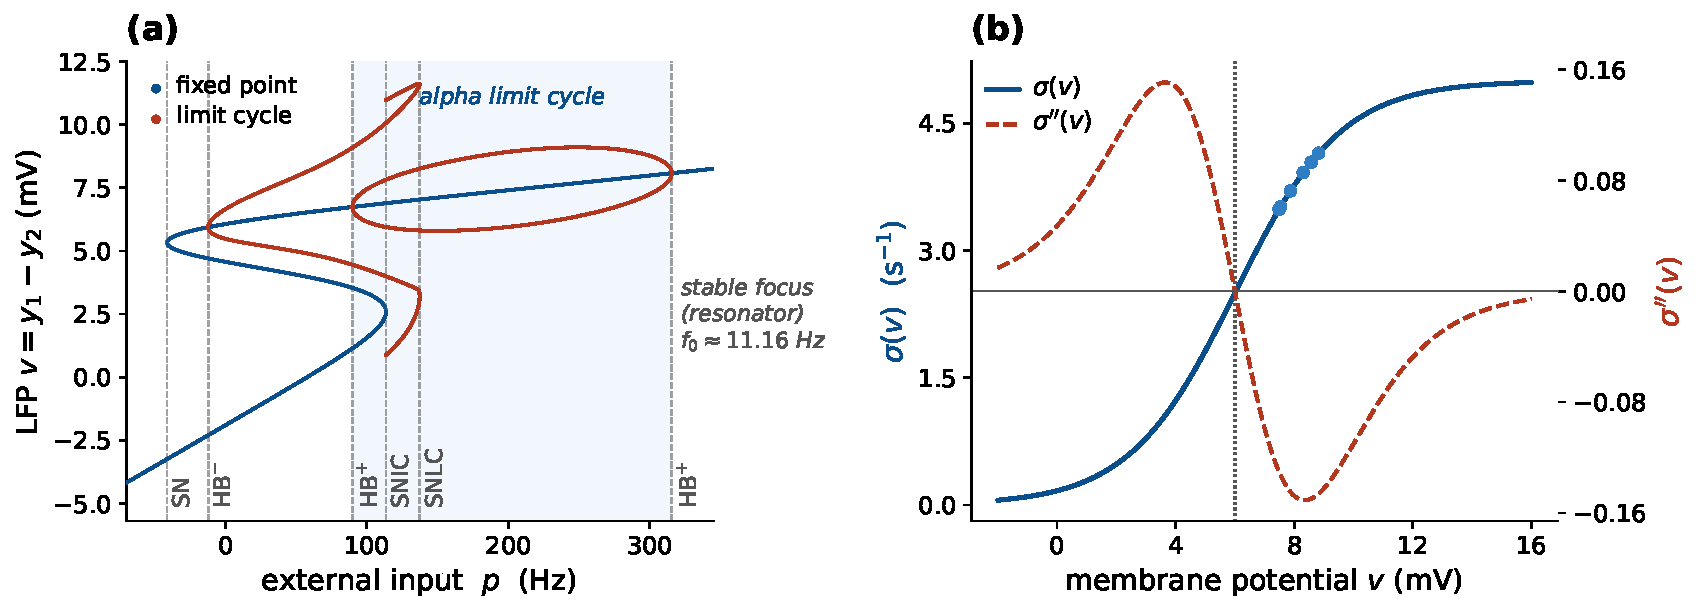
\includegraphics[width=\textwidth]{fig_bifurcation_sigmoid.pdf}
\caption{\textbf{JR operating states and sigmoid curvature.}
\emph{(a)} Numerical continuation of fixed points (blue) and cycle extrema
(red) against external drive $p$; solid branches are stable, faded branches
unstable. The alpha cycle lies between Hopf points near $90$ and
$316$~s$^{-1}$. Beyond the upper Hopf the fixed point is a stable focus,
with $f_0\approx11.16$~Hz. Markers identify saddle-nodes (SN), Hopf points
(HB$^\pm$), the saddle-node on an invariant circle (SNIC), and the
saddle-node of limit cycles (SNLC).
\emph{(b)} Sigmoid and curvature; dots mark the modeled operating points.}
\label{fig:bif}
\end{figure}

The open-loop sigmoid at fixed $v^*$ isolates detection; its signed lock-in
tests the curvature law. The closed-loop column measures recurrent gain over
an $(\Omega,p)$ grid. Controls test quadratic amplitude scaling on a well-damped
focus, abolition of the beat when the pyramidal sigmoid is replaced by its
tangent, and agreement of $\Sig'$ and $\Sig''$ with finite differences.
Field-free trajectories initialized near the fixed point check the continuation.

\subsection{Exact next-generation mean field (NMM2 PING)}\label{sec:nmm2-methods}
The pyramidal--interneuron network gamma (PING) circuit couples excitatory
and inhibitory MPR populations through second-order synapses
\cite{montbrio2015,ruffini2021nmm2,clusella2023}, using the Rosetta Stone
formulation shared with JR and laminar models \cite{ruffini2025rosetta}.
For population $X\in\{E,I\}$, $r_X$ is physical rate (ms$^{-1}$),
$v_X$ dimensionless mean voltage, and $\tau_X$ membrane time (ms).
With dots denoting physical-time derivatives,
\begin{equation}
\begin{aligned}
\tau_E\dot r_E&=\Delta/(\pi\tau_E)+2r_Ev_E, &\quad
\tau_E\dot v_E&=v_E^2+\bar\eta-(\pi\tau_E r_E)^2+\tau_E J\,(r_E^{\rm syn}-r_I^{\rm syn})+I_E(t),\\[2pt]
\tau_I\dot r_I&=\Delta/(\pi\tau_I)+2r_Iv_I, &\quad
\tau_I\dot v_I&=v_I^2+\bar\eta-(\pi\tau_I r_I)^2+\tau_I J\,(r_E^{\rm syn}-2r_I^{\rm syn}),
\end{aligned}
\label{eq:nmm2-ping}
\end{equation}
The synaptic rates $r_E^{\rm syn}=\hat K_a[r_E]$ and
$r_I^{\rm syn}=\hat K_g[r_I]$, with times $\tau_a$ and $\tau_g$,
obey the critically damped operator
$\tau_s^2\ddot r_{\rm syn}+2\tau_s\dot r_{\rm syn}+r_{\rm syn}=r$.
Here $J$ is dimensionless global gain; weights
$(w_{EE},w_{EI},w_{IE},w_{II})=(1,1,1,2)$ use target/source indices,
with doubled inhibitory self-coupling as the only asymmetry.
In the schematic, $\mathcal U_j(t)$ denotes neuron $j$'s total synaptic
and field input, and $J^*$ the coupling-induced Hopf.

The background $\bar\eta$ controls a supercritical Hopf opening a gamma
cycle, analogous to the JR alpha Hopf. The field enters the E-voltage
equation as $I_E(t)=\lambda_I E(t)$ \cite{ruffini2021nmm2}.
The instantaneous coupling $\lambda_I$ has units of normalized drive per V/m;
two tones at $f_c\mp\Delta f/2$ have amplitude $A_f$ in the same
dimensionless drive units as $\bar\eta$. We set $f_c=300$~Hz and sweep
$\Delta f$ through gamma. The membrane integrates each tone into an
excursion $A_f/(\omega\tau_E)$, which $v_E^2$ rectifies: access uses
$\tau_m=\tau_E$, without an assumed sigmoid.

We integrate with fixed-step RK4 ($\Delta t=0.05$~ms) and read out the lock-in
(Eq.~\eqref{eq:lockin}) of $r_E$ at $\Delta f$ over the $(\Delta f, \bar\eta)$ plane.
Parameters (Rosetta Stone PING \cite{ruffini2025rosetta}): $\Delta=1$, global coupling
$J=15$, $\tau_E=15$, $\tau_I=7.5$, $\tau_a=10$, $\tau_g=2.5$~ms, with $\bar\eta$ swept
through the supercritical Hopf at $\bar\eta_H=1.110$ ($f_0=54.0$~Hz), located by bisection
on the leading eigenvalue of the mean-field Jacobian. The simulations retain these
finite membrane times; Eq.~\eqref{eq:slow_synapse} characterizes the fast-membrane limit.

The resonance map varies $\bar\eta$ (Fig.~\ref{fig:nmm2_map}); the
J-curve varies $J$ at fixed $\bar\eta$ toward $J^*$ and measures the
peak rate lock-in over $\Delta f$ (Fig.~\ref{fig:nmm2_jcurve}).
The $J^*$ Hopf is located by the same eigenvalue bisection.
Unlike JR, the PING J-curve does not pin the operating point. At
$\bar\eta=0$, continuation tracks the critical pair defining $\gamma$,
even when another mode dominates. The linear reference includes the
state-dependent source and full transfer; grids, amplitude checks, and
normalizations are supplementary (\S\ref{supp:ping-runs}).

\ifjne\else
\subsection{PING coupling-sweep settings}\label{supp:ping-runs}
We compute the linear reference's
second-order source from the PING quadratic terms at the central carrier,
$300$~Hz, and apply the full linearized network response over $15$--$90$~Hz
in $0.025$~Hz steps. Using the distinct AM sidebands changes the peak gain by
less than $0.1\%$ across this sweep.

The simulated coupling sweep uses the AM surrogate, $A_f=8$, with $5$~s
settling and a $4$~s window. We search around each linear resonance, extending
the frequency grid until each sampled maximum is bracketed, and compare
amplitudes $A_f=2,4,8$ at nine couplings. Local parabolic interpolation changes
the sampled peaks by less than $1.3\%$. The figure scales the linear reference
to the median measured gain over $14.5<J<16$; the amplitude check instead
normalizes peak response divided by $A_f^2$ and linear gain to its value at
$A_f=2$, $J=15.53$. These normalizations compare gain variation with the detector coefficient
allowed to vary along this unpinned sweep.


\fi

Stability of the driven endpoint is checked using period-to-period perturbation
multipliers, direct perturbation decay, and a finite-time Lyapunov estimate;
settings and results are given in the supplement (\S\ref{app:ping-stability}).

\subsection{QIF spiking network (microscale of NMM2)}\label{sec:qif-methods}
To compare beat-locked and ongoing activity at the spike level, we simulate
the all-to-all QIF network whose infinite-population limit is
NMM2 \cite{montbrio2015,ruffini2025rosetta,clusella2023}, with $N=8000$
neurons per population and the PING parameters of Eq.~\eqref{eq:nmm2-ping}.
Single-neuron voltages $V_j$ spike at $V_{\rm peak}=100$ and reset to
$-V_{\rm peak}$ in model units. Excitabilities follow deterministic
quantiles of Lorentzian$(\bar\eta,\Delta)$; empirical rates drive the
second-order synapses. Genuine two-tone input enters E membranes because
spiking and threshold dynamics need not preserve surrogate equivalence
beyond perturbation theory.

At $f_c=300$~Hz and amplitude $A_f=35$ per tone, we use
$\bar\eta=0.85$, beat $55$~Hz, and $\bar\eta=1.5$, beat $42$~Hz.
These lie below and above the field-free Hopf
($\bar\eta_H=1.110$, $f_0=54.0$~Hz). Condition labels refer to that
field-free state; spectra and rate folds separate components without
establishing phase capture.

We \DIFdelbegin \DIFdel{also run }\DIFdelend \DIFaddbegin \DIFadd{repeat }\DIFaddend both conditions at $A_f=10$ \DIFdelbegin \DIFdel{per tone with the same measurement
settings. For $\bar\eta=0.85$, separate checks double the populationsize, double the measurement window,
or halve the integration step; further runs raise
$V_{\rm peak}$ to $200$ and $400$ at both time steps}\DIFdelend \DIFaddbegin \DIFadd{and test step, population, window,
and spike-cutoff sensitivity}\DIFaddend . An equal-RMS mean-field control replaces the
two tones by one $300$~Hz carrier \DIFdelbegin \DIFdel{with peak amplitude $\sqrt{2}A_f$, using the same duration: }\DIFdelend \DIFaddbegin \DIFadd{of peak amplitude $\sqrt2 A_f$;
}\DIFaddend both inputs have mean-square amplitude $A_f^2$\DIFdelbegin \DIFdel{over these windows. The carrier comparison starts from the
field-free equilibrium and uses $800$~ms settling and $800$~ms measurement,
with a $3200$~ms window to check spectral leakage
at the larger amplitude}\DIFdelend . \DIFaddbegin \DIFadd{The protocol and leakage
check are specified in the supplement (\S\ref{supp:qif-protocol}).
}\DIFaddend

The carrier-averaged stability calculation includes the drive-dependent
second-order DC source (supplement, \S\ref{app:qif-estimate}). Direct two-tone
integrations retain the beat and separately check the averaged prediction.

Euler integration uses $0.0025$~ms steps\DIFdelbegin \DIFdel{and $800$~ms settling, exceeding
four field-free relaxation times at $\bar\eta=0.85$ ($176$~ms). Measurements cover whole beat cycles to avoid phase-coverage bias:
$44$ at $55$~Hz and $34$ at $42$~Hz ($800$ and $810$~ms}\DIFdelend \DIFaddbegin \DIFadd{. Settling times, whole-cycle windows,
and convergence checks are specified in the supplement
(\S\ref{supp:qif-protocol}}\DIFaddend ).
We report the rate lock-in as modulation depth
$A_\Omega/\langle r_E\rangle$; an off/on ratio would divide by the
field-free floor. Single-neuron locking is measured by pairwise phase
consistency (PPC) at $\Delta f$, unbiased in spike count
\cite{vinck2010}, for neurons with at least ten spikes per window.

A cutoff-free check uses the equivalent theta-neuron equation,
$V_j=\tan(\theta_j/2)$, with interpolated crossings of $\theta_j=\pi$.
Separate step, population, and window checks test a predeclared $5\%$
rate-depth tolerance (supplement, \S\ref{supp:theta-pilot}). Quantitative
convergence remains unestablished; the finite network is interpreted qualitatively.
\ifjne\else
\subsection{A cutoff-free theta-neuron check}\label{supp:theta-pilot}
The change of variables $V_j=\tan(\theta_j/2)$ converts the QIF equation to
\[
\tau_X\dot\theta_j=(1-\cos\theta_j)
 +(1+\cos\theta_j)(\eta_j+U_X(t)),
\]
where $U_X$ is the same recurrent and external input as in the voltage model.
An upward crossing of $\theta=\pi$ emits a spike; wrapping by $2\pi$ replaces
the finite voltage cutoff and reset. We linearly interpolate the crossing
time for phase statistics. Empirical spike counts still drive the original
second-order synapses. Excitability quantiles, initial voltage, coupling,
carrier, and readouts are unchanged.

The pilot used $\bar\eta=0.85$, $A_f=10$, $f_c=300$~Hz, a $55$~Hz beat,
and $800$~ms settling. Before running it, we set a stopping rule: rate depth
must change by less than $5\%$ under separate step halving, population
doubling, and window doubling before extending this solver to carrier controls.
Table~\ref{tab:theta-pilot} gives every tested setting. Step and window changes
satisfy that criterion; population doubling does not, so the pilot stops.
No finite-network equal-RMS control was run.

\begin{table}[htbp]
\centering\small
\begin{tabular}{@{}lrrrrr@{}}
\toprule
Condition & $N$ per population & Step (ms) & Window (ms) & Mean E rate (Hz) & Beat depth\\
\midrule
Field off & 8000 & 0.0025 & 800 & 50.4 & 0.006\\
Two tones & 8000 & 0.0025 & 800 & 51.8 & 0.156\\
Half step & 8000 & 0.00125 & 800 & 51.8 & 0.155\\
Double population & 16000 & 0.0025 & 800 & 51.8 & 0.137\\
Double window & 8000 & 0.0025 & 1600 & 51.8 & 0.151\\
Exact mean field & $\infty$ & 0.0025 & 800 & 52.1 & 0.128\\
\bottomrule
\end{tabular}
\caption{Cutoff-free weak-drive checks. Depth is the rate lock-in divided by
mean rate. Relative to the two-tone baseline it changes by $-0.4\%$,
$-11.9\%$, and $-3.0\%$ under step, population, and window changes.
Only the baseline settings have a matched field-off run.}
\label{tab:theta-pilot}
\end{table}

Removing the cutoff raises the baseline depth from $0.093$ to $0.156$.
The three cutoff results are compatible with an inverse-cutoff correction:
a fit of $d_\infty-c/V_{\rm peak}$ gives $d_\infty=0.156$, with residuals
of about $0.002$. This agreement supports a cutoff contribution but does not
establish joint numerical convergence. Doubling the population moves the
theta result toward the exact mean field, while also increasing the largest
sampled Euler step in phase from about $1.5$ to $3.2$ radians. A combined
population and time-step limit remains untested.

Pooled spike-phase vector strength rises from $0.002$ without stimulation
to $0.068$--$0.077$ in the driven runs. Median per-neuron phase consistency
remains negative, from $-0.015$ to $-0.005$, and supplies no evidence for
strong individual phase locking. The finite network therefore supports the
presence of population-rate modulation; its quantitative weak-input depth
and agreement with the mean field remain unresolved.

\fi

\DIFaddbegin \ifjne\else
\subsection{\DIFadd{QIF integration and matched-carrier protocol}}\label{supp:qif-protocol}
\DIFadd{The finite network uses the PING model and observables defined in
\S\ref{sec:qif-methods}. The following settings support the weak-drive and
field-induced gamma comparisons.
}

\DIFadd{Euler integration uses $0.0025$~ms steps and $800$~ms settling, exceeding
four field-free relaxation times at $\bar\eta=0.85$ ($176$~ms).
Measurements cover whole beat cycles to avoid phase-coverage bias:
$44$ at $55$~Hz and $34$ at $42$~Hz ($800$ and $810$~ms).
}

\DIFadd{We also run both conditions at $A_f=10$ per tone with the same measurement
settings. For $\bar\eta=0.85$, separate checks double the population size,
double the measurement window, or halve the integration step; further runs raise
$V_{\rm peak}$ to $200$ and $400$ at both time steps. An equal-RMS
mean-field control replaces the two tones by one $300$~Hz carrier with peak
amplitude $\sqrt{2}A_f$, using the same duration: both inputs have mean-square
amplitude $A_f^2$ over these windows. The carrier comparison starts from the
field-free equilibrium and uses $800$~ms settling and $800$~ms measurement,
with a $3200$~ms window to check spectral leakage at the larger amplitude.
}

\DIFadd{A longer window reduces the single carrier's apparent $55$~Hz
depth from $0.011$ to $9.2\times10^{-5}$, while TI's stays at $0.30$--$0.31$;
the former is spectral leakage.
}

\fi

\DIFaddend \subsection{Coupling sweeps, timing, and the tACS control (Jansen--Rit)}
The JR sweeps vary coupling while keeping detection fixed. For each
connectivity $C$, we solve for the external drive $p(C)$ that holds the
field-free voltage at $v^*=8.30$~mV, then obtain damping and modal frequency
from the Jacobian. This fixes the background curvature without canceling
stimulation-induced mean shifts.

The gain sweep uses the AM surrogate; the timing comparison uses genuine
two tones and measures modulation and mean of the same pyramidal rate
$r_P=\Sig(v+s)$. The tACS control uses a direct sinusoid at the same beat
frequency and reads the same voltage lock-in as TI. Further controls match
tACS to TI's generated beat source and repeat the comparison with longer
settling and measurement windows. Waveforms, amplitudes, and run windows
are recorded together in the supplement.

\section{Results}
\subsection{The JR column generates and resonantly amplifies the beat}
An input containing only the two tones $f_c\mp\Delta f/2$ produces an output
oscillation at their $11.1$~Hz beat, near the column's alpha resonance
(Fig.~\ref{fig:bif}). The alpha peak is absent from the input spectrum
(Fig.~\ref{fig:demod}).

\begin{figure}[t!]
\centering
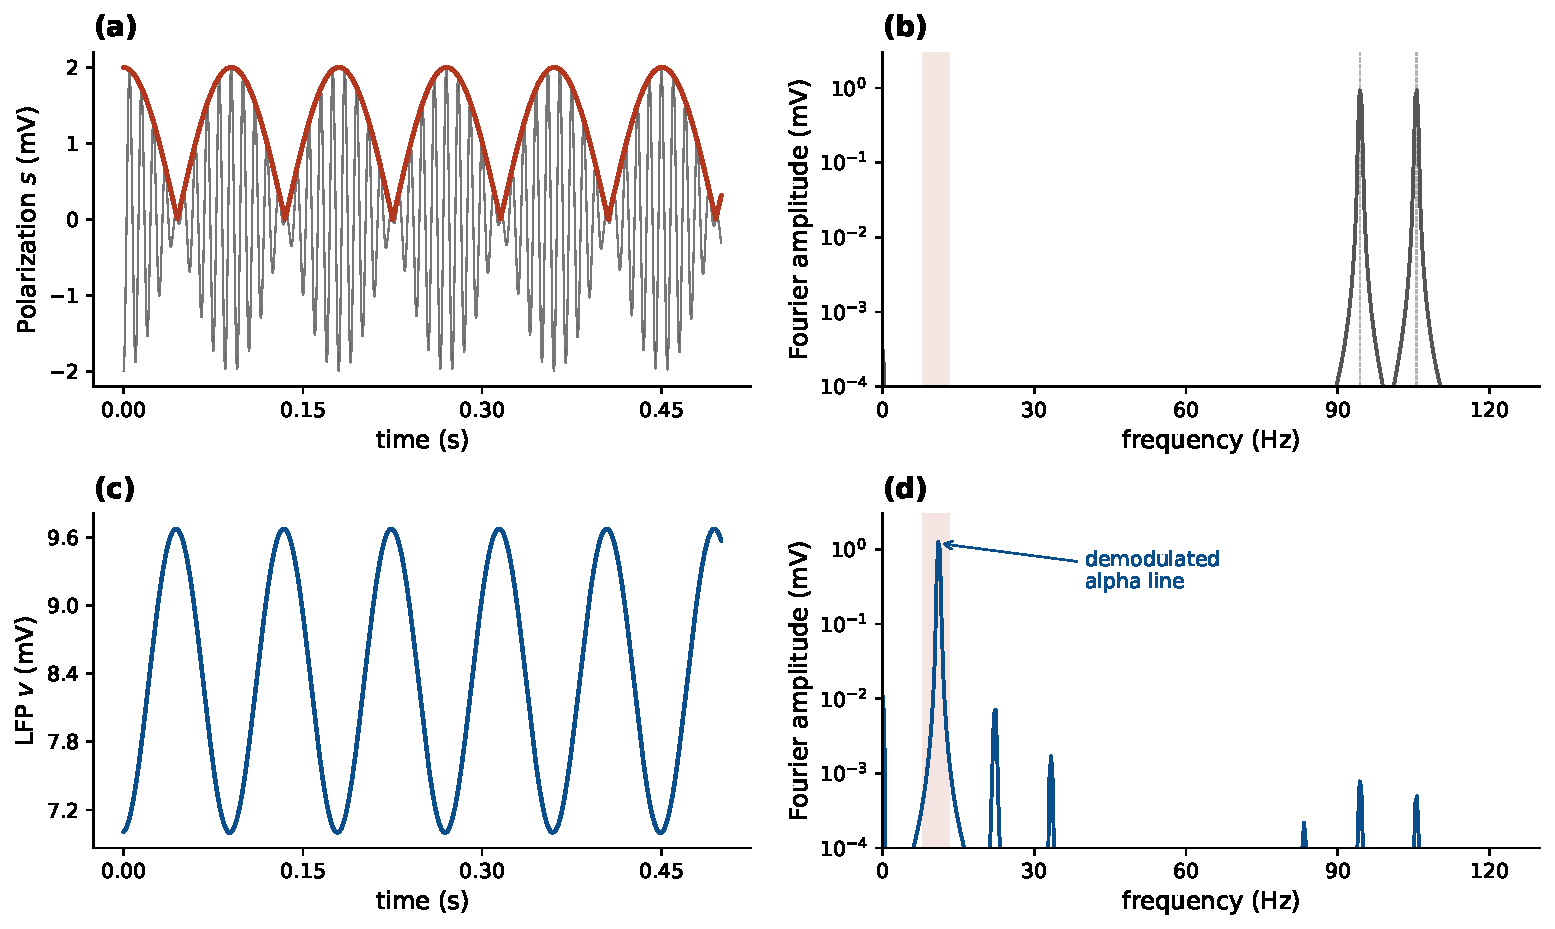
\includegraphics[width=\textwidth]{fig_demodulation_twotone.pdf}
\caption{\textbf{The JR column generates a beat absent from the input.}
\emph{(a)} Two equal tones at $94.45$ and $105.55$~Hz and their envelope,
$2\varepsilon|\cos(\Omega t/2)|$. \emph{(b)} Input spectrum: only the two
tones are present. The alpha-band floor is $1.6\times10^{-8}$ of their
amplitude, from finite-window leakage. \emph{(c,d)} The synaptic voltage
$v=y_1-y_2$ and its spectrum show the generated $11.1$~Hz beat.
The field-free column is a stable focus near its alpha Hopf.}
\label{fig:demod}
\end{figure}

In the stable-focus regime ($p>p_H$), the response is approximately Lorentzian
and its peak grows from $0.23$ to $0.43$ to $0.70$~mV toward the Hopf
(Fig.~\ref{fig:res}), as expected from the
$1/\gamma$ susceptibility. Without a drive the focus is silent at $\Omega$;
the nonlinearity generates that component and recurrence amplifies it.
The peak shifts with the driven operating state; the near-Hopf law gives
its leading gain, not its exact frequency. The coupling sweep tests that law
over a decade of damping.
On the alpha branch below $p_H$, the column free-runs at $f_0$, so the lock-in
can contain both driven and autonomous activity. The dominant output frequency
$f_{\rm out}$ then identifies a frequency-dominance region
(Fig.~\ref{fig:entrain}), without establishing phase capture.

\begin{figure}[t!]
\centering
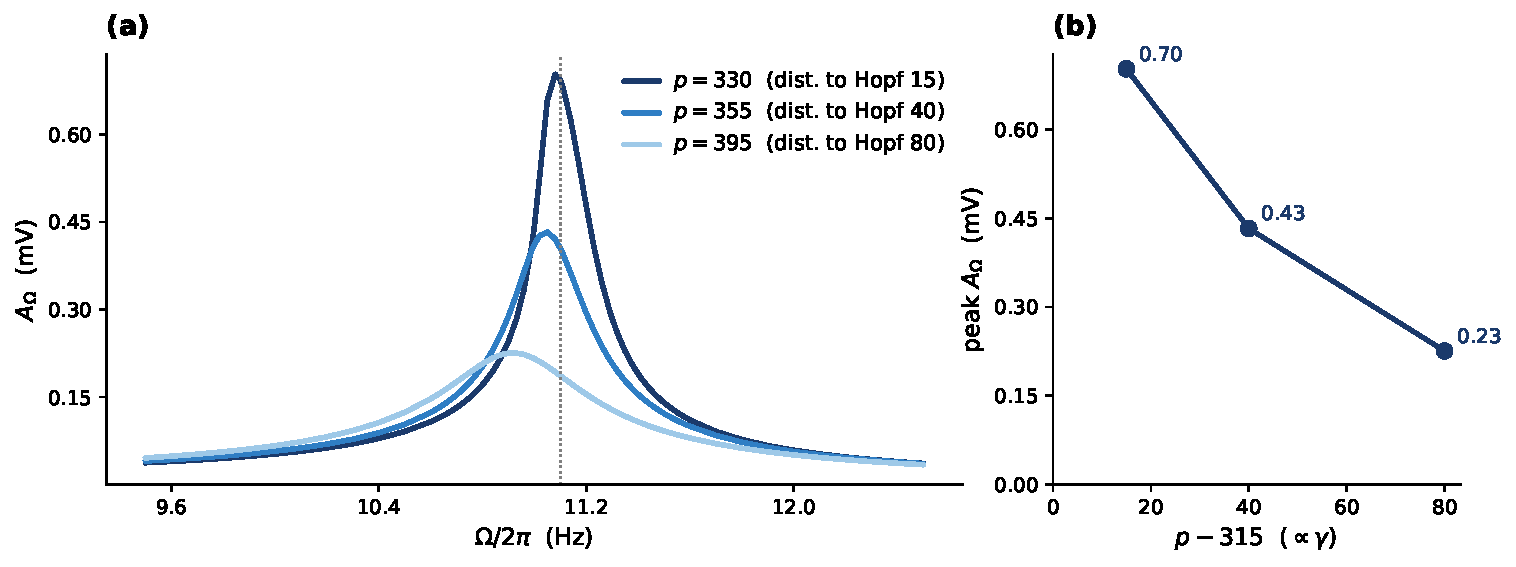
\includegraphics[width=\textwidth]{fig_resonance.pdf}
\caption{\textbf{The JR beat resonance sharpens toward the Hopf.}
Stable-focus response at $\varepsilon=0.3$~mV. \emph{(a)} Lock-in amplitude
against beat frequency; the finite-amplitude peak moves from $11.08$ to
$10.93$~Hz across the curves. \emph{(b)} Peak amplitude increases as $p$
approaches the upper Hopf from above. These three points show sharpening
and growth; the coupling sweep quantifies the $1/\gamma$ scaling and
its saturation.}
\label{fig:res}
\end{figure}

\subsection{Carrier independence and the kHz roll-off}
At fixed post-access polarization, the open-loop detector and near-Hopf
JR column are carrier-independent outside their natural band
(Fig.~\ref{fig:carrier}). At fixed applied field, the point-membrane
response instead falls as $1/f_c^2$ above its corner
(Fig.~\ref{fig:khz}); the sealed-cable estimate is compared with the
point-membrane cases in Fig.~\ref{fig:feasibility}a.

\begin{figure}[t!]
\centering
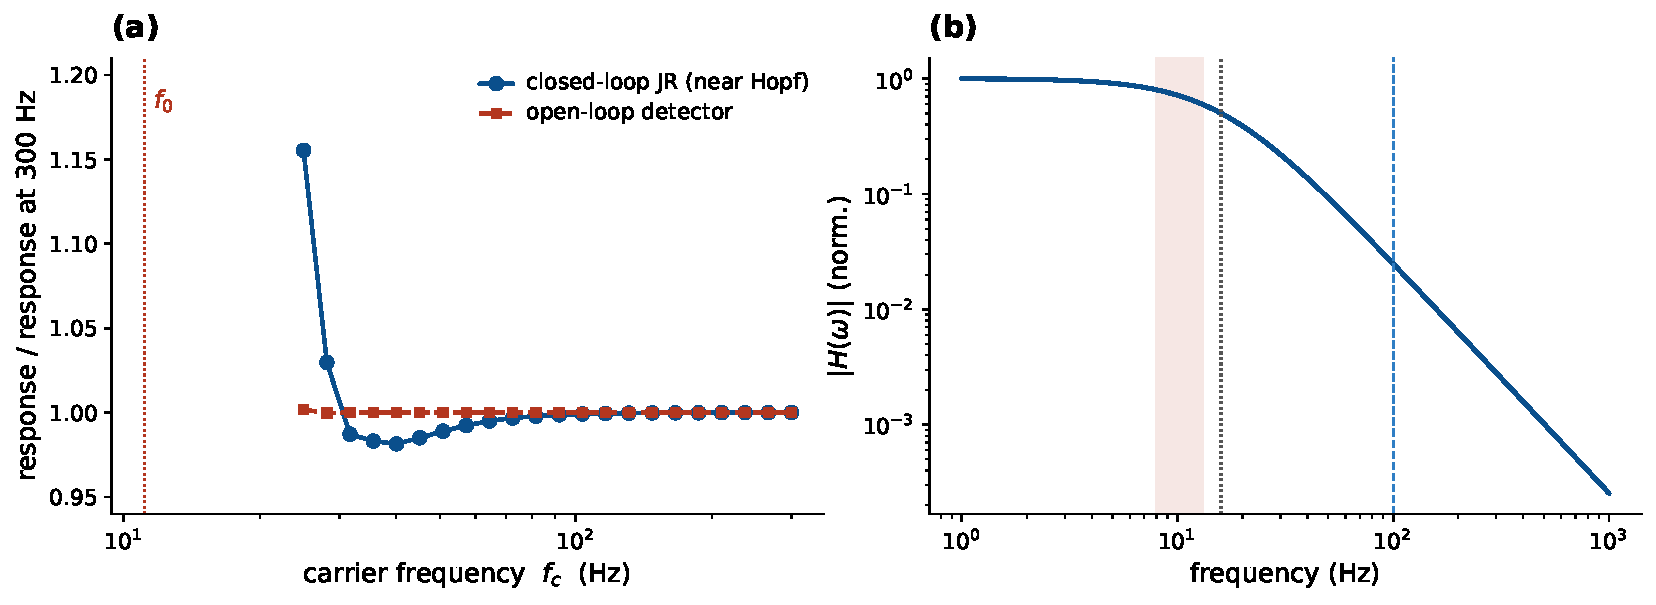
\includegraphics[width=\textwidth]{fig_carrier_independence.pdf}
\caption{\DIFdelbeginFL \DIFdelFL{\textbf{The demodulated response is carrier-independent at fixed polarization (Jansen--Rit).} }\DIFdelendFL \DIFaddbeginFL \DIFaddFL{\textbf{JR carrier independence at fixed polarization.}
}\DIFaddendFL \emph{(a)} \DIFdelbeginFL \DIFdelFL{The demodulated response is
nearly flat across carrier frequency }\DIFdelendFL \DIFaddbeginFL \DIFaddFL{Open- and closed-loop beat responses over }\DIFaddendFL $f_c=25$--$300$~Hz\DIFdelbeginFL \DIFdelFL{for the open-loop detector
and for the closed-loop JR near the Hopf}\DIFdelendFL ,
with deviations \DIFdelbeginFL \DIFdelFL{as $f_c$ approaches }\DIFdelendFL \DIFaddbeginFL \DIFaddFL{near }\DIFaddendFL the natural band. Each \DIFdelbeginFL \DIFdelFL{curve }\DIFdelendFL is normalized by its own
\DIFdelbeginFL \DIFdelFL{response at }\DIFdelendFL $300$~Hz \DIFaddbeginFL \DIFaddFL{response}\DIFaddendFL : $0.00670$~s$^{-1}$ open loop and $0.512$~mV closed
loop\DIFdelbeginFL \DIFdelFL{. Their ratio is }\DIFdelendFL \DIFaddbeginFL \DIFaddFL{, giving }\DIFaddendFL a rate-to-voltage transfer of $76.4$~mV\,s.
\DIFdelbeginFL \DIFdelFL{The open-loop
carrier independence follows to leading order from Eq.~\eqref{eq:demod}. }\DIFdelendFL \emph{(b)} \DIFdelbeginFL \DIFdelFL{The second-order-synapse low-pass }\DIFdelendFL \DIFaddbeginFL \DIFaddFL{Relative synaptic transfer }\DIFaddendFL $|H_s(\omega)|/|H_s(0)|$\DIFdelbeginFL \DIFdelFL{passes the envelope ($\sim$0.7) }\DIFdelendFL \DIFaddbeginFL \DIFaddFL{: about
$0.7$ at $10$~Hz }\DIFaddendFL and \DIFdelbeginFL \DIFdelFL{suppresses the }\DIFdelendFL \DIFaddbeginFL \DIFaddFL{$2.5\%$ at }\DIFaddendFL $100$~Hz\DIFdelbeginFL \DIFdelFL{carrier ($\sim$2.5\%)}\DIFdelendFL . Dotted\DIFdelbeginFL \DIFdelFL{line}\DIFdelendFL : synaptic corner
\DIFdelbeginFL \DIFdelFL{$a/2\pi\!\approx\!16$}\DIFdelendFL \DIFaddbeginFL \DIFaddFL{$a/(2\pi)\approx16$}\DIFaddendFL ~Hz; shaded\DIFdelbeginFL \DIFdelFL{band}\DIFdelendFL : \DIFdelbeginFL \DIFdelFL{envelope (}\DIFdelendFL $8$--$13$~Hz \DIFdelbeginFL \DIFdelFL{)}\DIFdelendFL \DIFaddbeginFL \DIFaddFL{beat band}\DIFaddendFL ; dashed\DIFdelbeginFL \DIFdelFL{line}\DIFdelendFL : \DIFdelbeginFL \DIFdelFL{$100$~Hz }\DIFdelendFL carrier.}
\label{fig:carrier}
\end{figure}

With an explicit first-order access state per modeled compartment before
the sigmoid, the full JR column demodulates and resonates in the assumed
$\tau=0.2$~ms case (Fig.~\ref{fig:khz_direct}a). Genuine tones centered
at $2$~kHz generate the absent $10.914$~Hz beat, with analytic access
factor $|H_m|^2=0.137$ (Fig.~\ref{fig:khz_twotone}). These are consequences
of the assumed access time and coupling; neither is calibrated by the simulation.

Figure~\ref{fig:feasibility} converts this access assumption into a source
budget. With $\varepsilon_j=\lambda_0 E_j|H_m(\omega_j)|$, the equivalent
direct beat input is $\varepsilon_{\rm eq}=Y_\Omega/\Sig'$, before recurrent
gain. At $2$~kHz, $\tau_m=0.2$~ms, $\lambda_0=0.5$~mV per V/m, and
$0.5$~V/m per tone, it has magnitude $1.36~\mu$V; the steady equivalent
is nearly identical. Reducing the assumed coupling to $0.15$ scales these
sources by $0.09$. Thus the matched-polarization $2$--$5\%$ comparison does
not carry over unchanged to matched applied fields.

At equal fields, the $0.2$~ms point-membrane model predicts a narrowband
$9/1$~kHz source ratio of $0.020$. The limit $1/81$ applies only when
both bands lie above their access corners. A sealed long cable instead
approaches a $1/9$ ratio. These calculations locate conditional input budgets;
they do not calibrate the biological transfer.
\DIFdelbegin \DIFdel{The dynamic QIF equations
already include membrane access, so this filter must not be applied again.
}\DIFdelend

\begin{figure}[t!]
\centering
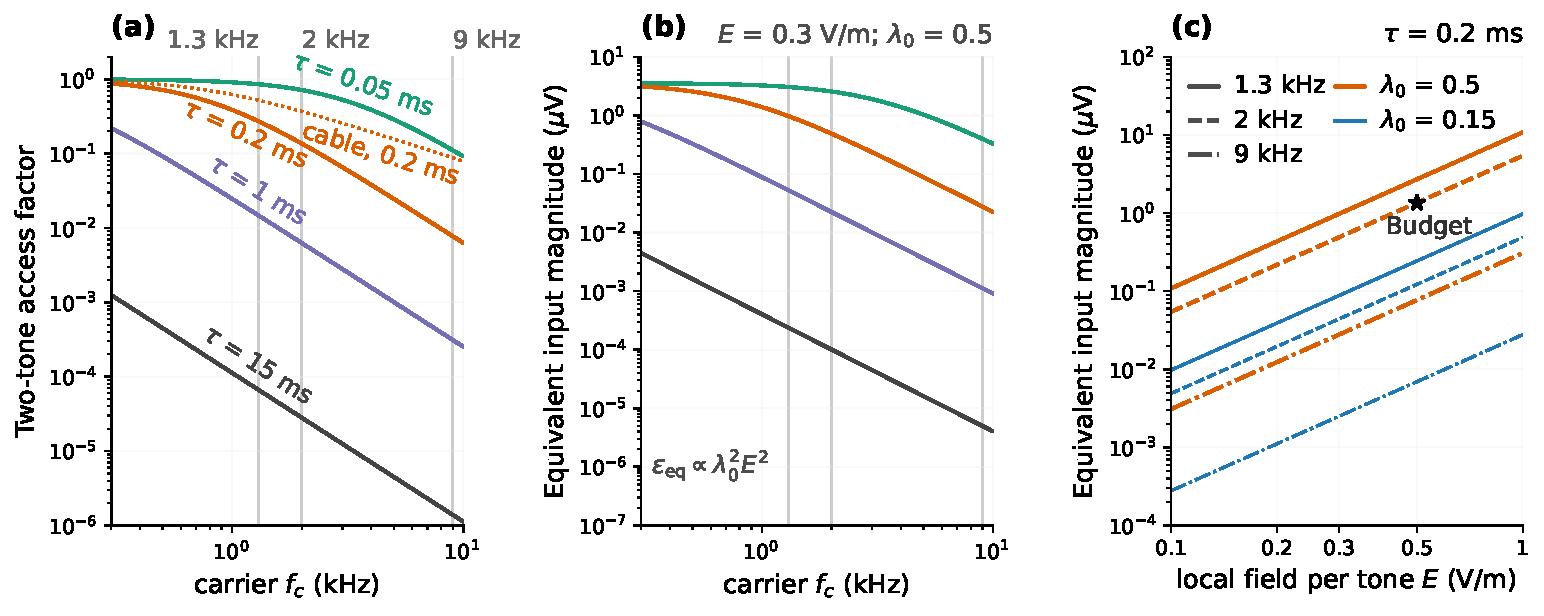
\includegraphics[width=\textwidth]{fig_feasibility_khz.pdf}
\caption{\textbf{Carrier access sets the source budget at fixed field.}
\emph{(a)} Exact two-tone access factor for tones $10$~Hz apart; dotted,
sealed-cable approximation at $0.2$~ms.
\emph{(b)} Beat-equivalent direct polarization magnitude at the pinned JR state,
$E=0.3$~V/m per tone and $\lambda_0=0.5$~mV per V/m. For $\lambda_0=0.15$,
multiply by $0.09$.
\emph{(c)} Field dependence at $0.2$~ms for both couplings; star marks
the illustrative budget. All sources are leading-order, before recurrent
gain; $\lambda_0$ and the access time are assumptions.}
\label{fig:feasibility}
\end{figure}

\subsection{\DIFdelbegin \DIFdel{The nonlinearity is the detector: the
}%DIFDELCMD < \texorpdfstring{$\Sig''$}{sigma''} %%%
\DIFdelend \DIFaddbegin \DIFadd{Sigmoid }\DIFaddend curvature \DIFdelbegin \DIFdel{law and its controls}\DIFdelend \DIFaddbegin \DIFadd{predicts the JR beat source}\DIFaddend }\label{sec:results-curvature}
The signed open-loop \DIFdelbegin \DIFdel{response tracks $\half\Sig''(v^*)\varepsilon^2 m$ across the
operating range}\DIFdelend \DIFaddbegin \DIFadd{beat follows $\half\Sig''(v^*)\varepsilon^2m$}\DIFaddend , vanishing
and reversing \DIFdelbegin \DIFdel{sign }\DIFdelend \DIFaddbegin \DIFadd{phase }\DIFaddend at the inflection \DIFdelbegin \DIFdel{$v_0$
}\DIFdelend (Fig.~\ref{fig:opp})\DIFdelbegin \DIFdel{---demodulation is the sigmoid-curvature term of
Eq. ~\eqref{eq:demod}, and the }\DIFdelend \DIFaddbegin \DIFadd{. The }\DIFaddend closed-loop
\DIFdelbegin \DIFdel{operating points sit where $\Sig''$ is large and negative.
Changing its sign reverses the source phase; at }\DIFdelend \DIFaddbegin \DIFadd{examples occupy the negative-curvature flank. At }\DIFaddend matched network
susceptibility, \DIFdelbegin \DIFdel{its magnitude sets the same resonant-gain calculation on either flank }\DIFdelend \DIFaddbegin \DIFadd{either flank follows the same gain law, with opposite source
phase when the curvature changes sign}\DIFaddend .

\begin{figure}[p]
\centering
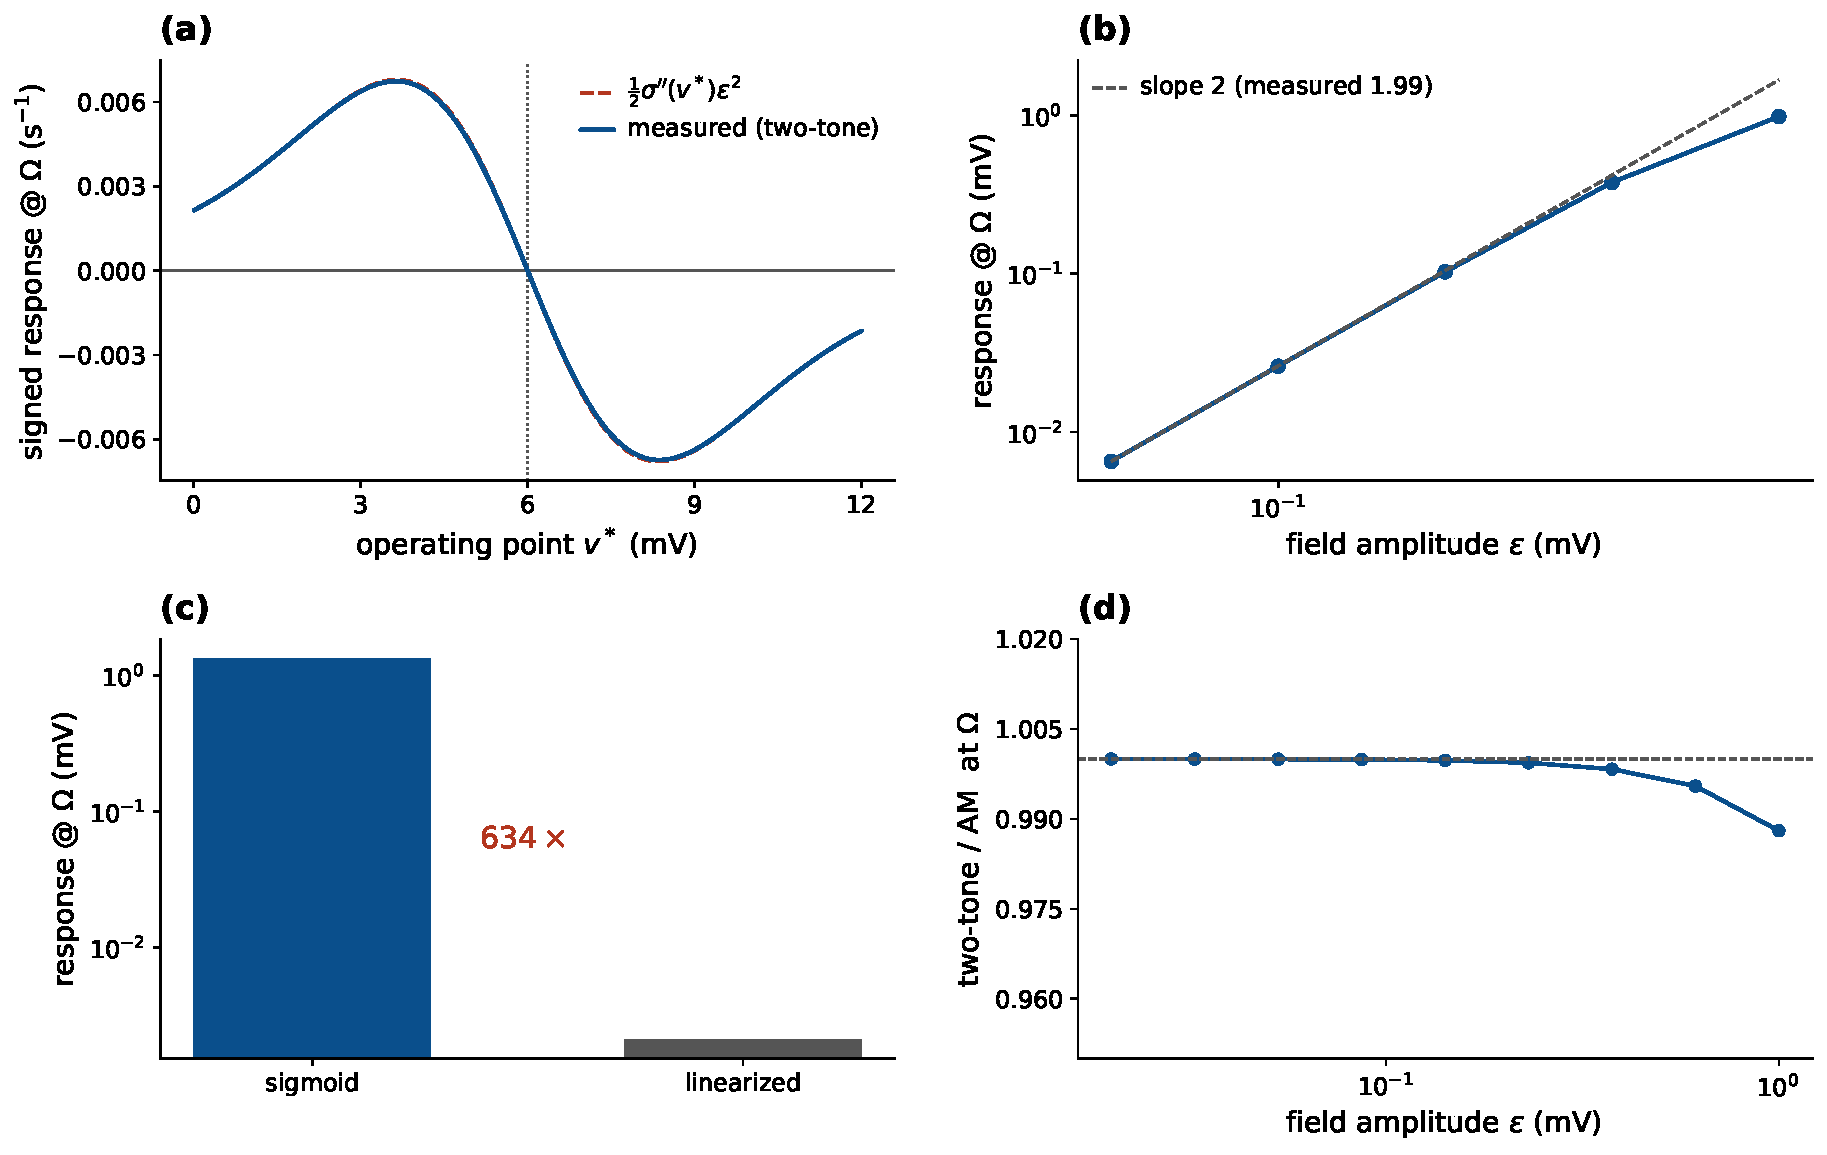
\includegraphics[width=\textwidth]{fig_curvature_twotone.pdf}
\caption{\textbf{Curvature determines the JR detector.}
\emph{(a)} The signed open-loop beat follows
$\Sig''(v^*)\varepsilon^2/2$ within $0.9\%$, vanishing and reversing sign
at $v_0$. \emph{(b)} The recurrent response has amplitude slope $1.99$.
\emph{(c)} Linearizing the receiving sigmoid reduces the beat $634$-fold.
\emph{(d)} Open-loop two-tone/AM beat ratio at $v^*=8$~mV:
$1.0000$ at $0.02$~mV and $0.988$ at $1$~mV. This checks the leading
local source, not the nonlinear recurrent response near the Hopf.}
\label{fig:opp}
\end{figure}

In the recurrent column, the response scales quadratically at small drive
(log--log slope $1.99$, measured as in \S\ref{sec:transduction-methods}),
and linearizing the field-receiving sigmoid reduces it
from $1.34$ to $0.0021$~mV (Fig.~\ref{fig:opp}b,c). The open-loop surrogate
comparison in panel~(d) supports its use for leading-order beat sweeps, with
the waveform and near-Hopf limitations specified in \S\ref{sec:waveforms}.

\subsection{Realistic-head comparison of envelope and quadratic maps}\label{sec:fem-results}
In this single-subject geometric illustration, changing the current ratio
moves the envelope and mean-square ROI centroids in opposite directions,
while the quadratic beat map only rescales. Each centroid uses the top 10\%
of hippocampal nodes; it is not a whole-brain maximum.
Figure~\ref{fig:fem} compares the maps of Table~\ref{tab:transduction-maps}
for the Violante montage in IXI002, using the same polarizations and fixed
1:1 projection (\S\ref{sec:fem-methods}).

Table~\ref{tab:fem-summary} summarizes the 1:1 to 1:3 change. The pair-current
product falls from $4$ to $3$~mA$^2$, so the quadratic excursion falls to $75\%$
of its value at every node, to machine precision. Its normalized map, contrast, and focus
are unchanged. The envelope focus moves anteriorly, toward the pair whose current
falls; the mean-square focus moves posteriorly, toward the pair whose current rises.
At 1:1, degree matching reduces the quadratic contrast to $1.08$, below the
envelope's $1.22$, while mean-square polarization favors the reference. These modest contrasts
separate geometric predictions but do not establish physiological deep selectivity.

\begin{table}[htbp]
\centering\small
\caption{\textbf{Hippocampal maps under current-ratio changes.} Means refer to the
ROI; contrasts are ROI/reference 95th-percentile ratios. Parentheses give
square-root, degree-matched contrasts. Focus shifts use the top 10\% of ROI
nodes, with anterior positive; ranges over other fractions are supplementary.}
\label{tab:fem-summary}
\begin{tabular}{@{}lrrrrr@{}}
\toprule
Map & Mean, 1:1 & Contrast, 1:1 & Contrast, 1:3 & Mean change & Focus shift\\
\midrule
Envelope & $0.16$ mV & $1.22$ & $0.95$ & $-45\%$ & $+2.5$ mm\\
Quadratic beat & $0.018$ mV$^2$ & $1.17$ ($1.08$) & $1.17$ ($1.08$) & $-25\%$ & $0$ mm\\
Mean square & $0.0094$ mV$^2$ & $0.92$ ($0.96$) & $0.90$ & $+24\%$ & $-4.5$ mm\\
\bottomrule
\end{tabular}
\end{table}

The \DIFdelbegin \DIFdel{sweep shows two kinds of steering (Fig.~\ref{fig:fem}e,f). The envelope ratio peaks
near balance ($1.24$ at a posterior share of $0.525$) and falls to $0.89$--$0.94$ at
the extremes. Its focus moves only while the two carriers are comparable
inside the hippocampus . At a posterior share of $0.6$ or more,}\DIFdelend \DIFaddbegin \DIFadd{envelope focus moves while }\DIFaddend the \DIFdelbegin \DIFdel{anterior pair is the weaker carrier at more than 96\% of hippocampal nodes; at $0.4$ or less, the posterior pair is. The
envelope map then equals twice the weaker pair's polarization }\DIFdelend \DIFaddbegin \DIFadd{carrier polarizations are comparable
within the hippocampus (Fig.~\ref{fig:fem}e,f). With greater imbalance,
the weaker carrier determines the envelope }\DIFaddend over most of the ROI, and
\DIFdelbegin \DIFdel{its measured focus changes little with further imbalance }\DIFdelend \DIFaddbegin \DIFadd{further imbalance changes its amplitude more than its focus. The envelope
contrast peaks at $1.24$ near balance. The mean-square focus instead moves
continuously toward the increasingly weighted pair; the quadratic map
retains one normalized pattern. Detailed transition points and ranges are
in the supplement (\S\ref{supp:fem-sensitivities})}\DIFaddend .
\DIFdelbegin \DIFdel{The focus of $\mathcal I$ moves
continuously instead, from $1.5$~mm anterior at a posterior share of $0.1$ to $6.3$~mm
posterior at $0.9$, while its ratio stays between $0.79$ and $0.94$ ($0.89$--$0.97$
degree-matched). The quadratic excursion keeps one ratio and one focus across the whole sweep.
}\DIFdelend

The isotropic beat map (Fig.~\ref{fig:fem}d,g) has a target-to-reference ratio of $1.18$
($1.08$ degree-matched), close to that of the fixed-direction quadratic map. It also
scales with $I_1^{\rm pair}I_2^{\rm pair}$, so the current ratio cannot steer it either.

Across all 32 combinations of montage, label, tissue definition, and focus
fraction, the envelope shift remains anterior, the mean-square shift posterior,
and the quadratic beat shift zero. Radial projections preserve those directions
but change absolute contrasts more than the atlas label does (supplement,
\S\ref{supp:fem-sensitivities}).
\ifjne\else
\subsection{Sensitivity of focus displacement}\label{supp:fem-sensitivities}
The spatial ordering in the article persists across montage, labeling, tissue,
and focus-fraction choices. Table~\ref{tab:fem-sensitivities} gives the ranges;
orientation changes absolute contrast more than the atlas label in this subject.
For the reference projection and label, the top-5--50\% focus moves
$2.2$--$4.0$~mm anteriorly for the envelope and $2.4$--$8.2$~mm posteriorly
for mean-square polarization.

\DIFaddbegin \DIFadd{The sweep shows two kinds of steering (Fig.~\ref{fig:fem}e,f). The envelope ratio peaks
near balance ($1.24$ at a posterior share of $0.525$) and falls to $0.89$--$0.94$ at
the extremes. Its focus moves only while the two carriers are comparable inside the
hippocampus. At a posterior share of $0.6$ or more, the anterior pair is the weaker
carrier at more than 96\% of hippocampal nodes; at $0.4$ or less, the posterior pair is. The
envelope map then equals twice the weaker pair's polarization over most of the ROI,
and its measured focus changes little with further imbalance. The focus of $\mathcal I$ moves
continuously instead, from $1.5$~mm anterior at a posterior share of $0.1$ to $6.3$~mm
posterior at $0.9$, while its ratio stays between $0.79$ and $0.94$ ($0.89$--$0.97$
degree-matched). The quadratic excursion keeps one ratio and one focus across the
whole sweep.
}

\DIFaddend \begin{table}[htbp]\centering\small
\caption{Focus displacement from 1:1 to 1:3. Envelope shifts are anterior;
mean-square shifts are posterior. The quadratic beat shift is zero in every case.
Contrasts quoted in the last column are raw 1:1 envelope/quadratic contrasts.}
\label{tab:fem-sensitivities}
\begin{tabular}{@{}lrrl@{}}
\toprule
Sensitivity & Envelope (mm) & Mean square (mm) & Contrasts\\
\midrule
Atlas label & $2.0$--$3.8$ & $3.2$--$5.9$ & $1.17$ / $1.04$\\
Radial direction & $1.9$--$2.8$ & $2.0$--$3.7$ & $1.62$ / $1.97$\\
All 32 combinations & $0.7$--$8.1$ & $0.5$--$10.6$ & \\
\bottomrule
\end{tabular}
\end{table}

\fi

\begin{figure}[htbp]
\centering
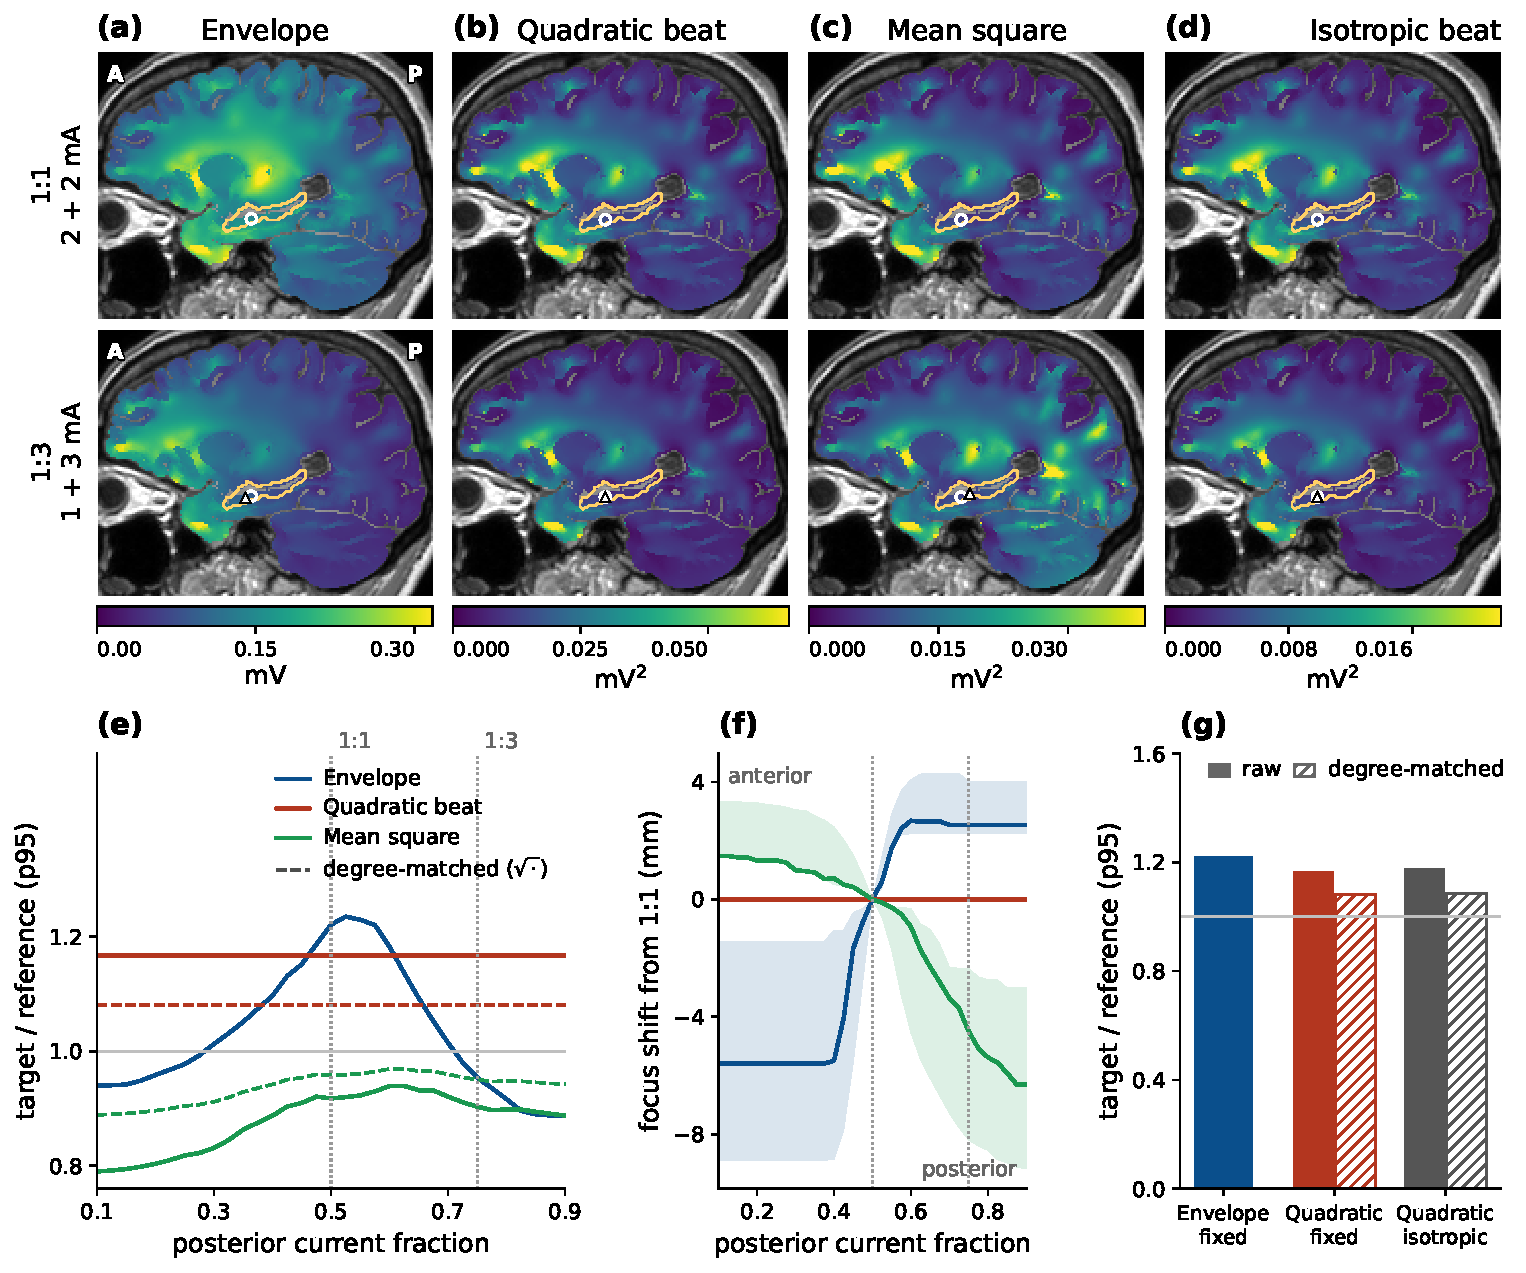
\includegraphics[width=\textwidth]{fig_fem.pdf}
\caption{\textbf{Envelope and quadratic maps in IXI002.}
Violante montage; left hippocampus outlined in gold, anterior to the left.
\emph{(a--d)} Sagittal maps at $2+2$~mA (top) and $1+3$~mA (bottom):
envelope excursion, quadratic excursion, mean-square polarization, and
isotropic beat. The first three use the fixed 1:1 envelope-maximizing
direction. Each color scale ends at its 1:1 gray-matter 99th percentile.
Circles and triangles mark the projected centroids of the top 10\% of ROI
nodes at 1:1 and 1:3, not whole-brain maxima.
\emph{(e)} Target-to-reference contrast; dashed curves use square-root
maps to match degree. \emph{(f)} Anterior focus displacement: top 10\%
(line), range over 5--50\% (band). \emph{(g)} Contrasts at 1:1, raw
(solid) and degree-matched (hatched).
The reference is gray matter outside the ROI. All maps precede detector
gain: $\mathcal I$ weights $Y_{\rm DC}=\Sig''\mathcal I/2$, but does not set its sign.}
\label{fig:fem}
\end{figure}

\subsection{Coupling sets the gain at fixed detection}\label{sec:jcurve}
With $v^*=8.30$~mV pinned by adjusting $p(C)$, the curvature and open-loop
beat $A_{\rm open}\simeq\half|\Sig''(v^*)|\varepsilon^2m$ stay fixed.
As $C\to C^*\approx137$, the damping tends to zero, the beat response
grows about $30$-fold, and its resonance sharpens (Fig.~\ref{fig:jcurve}a,b).
This is a network effect: the local detector curvature is fixed while
the recurrent transfer changes.
The rate-to-voltage gain $A_\Omega/A_{\rm open}$ (mV\,s) follows
$1/\gamma$ before saturating (panel~c). Approaching the Hopf through $p$
gives similar leading scaling. Finite-distance gains can differ because
modal frequencies and input--output projections vary along each path.

\begin{figure}[t!]
\centering
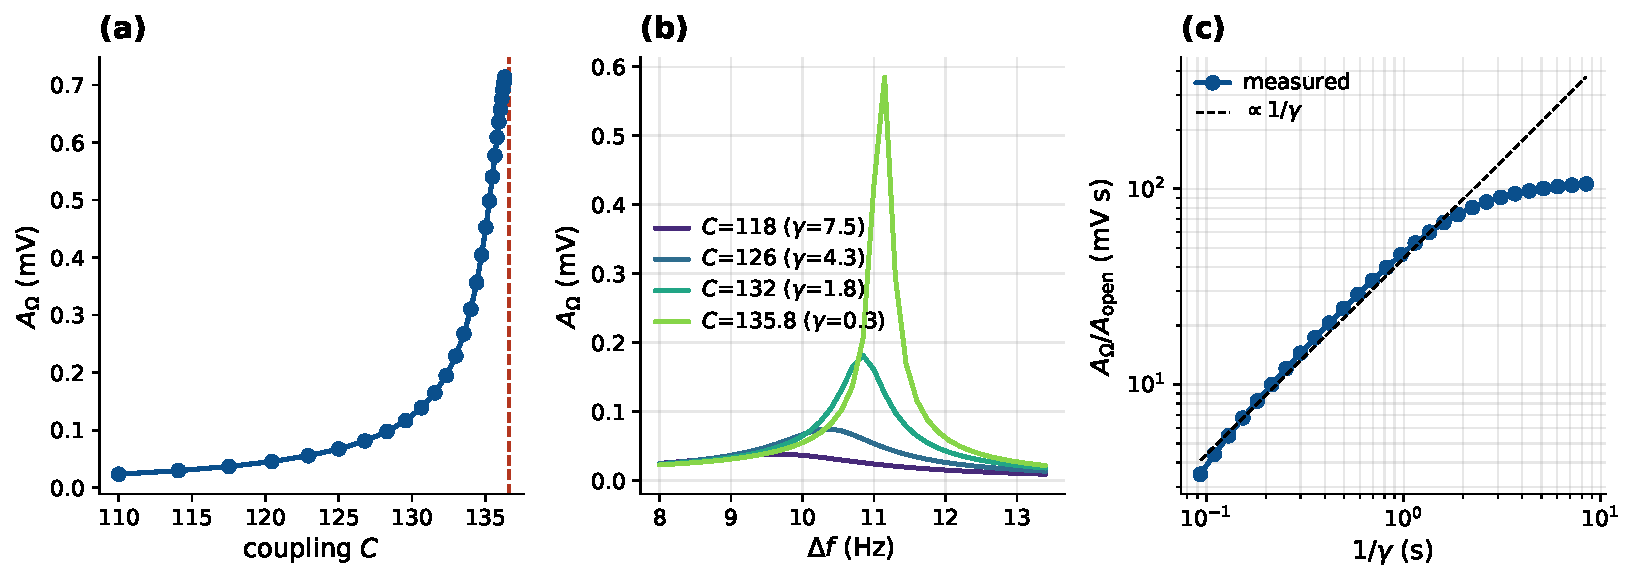
\includegraphics[width=\textwidth]{fig_jcurve.pdf}
\caption{\DIFdelbeginFL \DIFdelFL{\textbf{Coupling controls the amplification at fixed detection (Jansen--Rit).}
The input is the }\DIFdelendFL \DIFaddbeginFL \DIFaddFL{\textbf{JR coupling controls amplification at fixed detection.}
}\DIFaddendFL AM surrogate\DIFdelbeginFL \DIFdelFL{of }\DIFdelendFL \DIFaddbeginFL \DIFaddFL{, }\DIFaddendFL Eq.~\eqref{eq:amsur}\DIFdelbeginFL \DIFdelFL{.
The field-free operating point $v^*$ is pinned by co-solving }\DIFdelendFL \DIFaddbeginFL \DIFaddFL{; adjusting }\DIFaddendFL $p(C)$ \DIFaddbeginFL \DIFaddFL{pins the field-free
state}\DIFaddendFL , \DIFdelbeginFL \DIFdelFL{so }\DIFdelendFL \DIFaddbeginFL \DIFaddFL{curvature }\DIFaddendFL $\Sig''(v^*)=-0.151$~s$^{-1}$mV$^{-2}$\DIFaddbeginFL \DIFaddFL{, }\DIFaddendFL and \DIFaddbeginFL \DIFaddFL{open-loop
source }\DIFaddendFL $A_{\rm open}$\DIFdelbeginFL \DIFdelFL{are held constant throughout}\DIFdelendFL . \DIFdelbeginFL \DIFdelFL{\emph{(a)} }\DIFdelendFL \DIFaddbeginFL \DIFaddFL{\emph{(a,b)} }\DIFaddendFL The \DIFdelbeginFL \DIFdelFL{demodulated $A_\Omega$ }\DIFdelendFL \DIFaddbeginFL \DIFaddFL{response }\DIFaddendFL grows \DIFaddbeginFL \DIFaddFL{and sharpens }\DIFaddendFL as
\DIFdelbeginFL \DIFdelFL{the
coupling }\DIFdelendFL $C$ approaches the Hopf $C^*$ from the stable-focus side ($\gamma>0$).
\DIFdelbeginFL \DIFdelFL{\emph{(b)} The envelope resonance
sharpens and grows as $C\!\to\!C^*$. }\DIFdelendFL \emph{(c)} \DIFdelbeginFL \DIFdelFL{The network }\DIFdelendFL \DIFaddbeginFL \DIFaddFL{Rate-to-voltage }\DIFaddendFL gain $A_\Omega/A_{\rm open}$ \DIFdelbeginFL \DIFdelFL{, in }\DIFdelendFL \DIFaddbeginFL \DIFaddFL{(}\DIFaddendFL mV\,s\DIFdelbeginFL \DIFdelFL{, }\DIFdelendFL \DIFaddbeginFL \DIFaddFL{) }\DIFaddendFL follows
$1/\gamma$ (dashed) \DIFdelbeginFL \DIFdelFL{and saturates near the
bifurcation}\DIFdelendFL \DIFaddbeginFL \DIFaddFL{before saturating}\DIFaddendFL .}
\label{fig:jcurve}
\end{figure}

\subsection{\DIFdelbegin \DIFdel{The resonance amplifies the envelope-locked }\DIFdelend \DIFaddbegin \DIFadd{Resonance favors beat }\DIFaddend modulation \DIFdelbegin \DIFdel{more than }\DIFdelend \DIFaddbegin \DIFadd{over }\DIFaddend the mean \DIFdelbegin \DIFdel{rate}\DIFdelend \DIFaddbegin \DIFadd{shift}\DIFaddend }\label{sec:timing}
In the pinned JR coupling sweep, genuine two tones at $\Delta f=f_0$
increase modulation of $r_P=\Sig(v+s)$ by $13.2$-fold ($26$ to $339$~mHz),
following $1/\gamma$ before saturation. The same rate's mean shift grows
$4.4$-fold ($-1.8$ to $-7.7$~mHz), remaining below $0.2\%$ of its
$3.9$~Hz baseline (Fig.~\ref{fig:timing}). Their magnitude ratio rises
from $14.5$ to $58$ near $\gamma=1$~s$^{-1}$, then falls to $44$ as
the amplified oscillation rectifies. In this weakly driven regime, a small
mean change accompanies larger beat modulation, consistent with primate observations
\cite{vieira2024}, with both compared in rate units. The surrogate
comparison is supplementary (\S\ref{supp:waveform-checks}).

The \DIFdelbegin \DIFdel{demodulator feeds the network a constant term and a line at the beat $\Omega$
(Eq.~\eqref{eq:taylor}), and the transfer $G(\Omega)$ of Eq.~\eqref{eq:gain} treats them
differently}\DIFdelend \DIFaddbegin \DIFadd{detector's steady and beat sources meet different transfers}\DIFaddend :
$|G(\omega_0)|\propto1/(2\gamma\omega_0)$ \DIFdelbegin \DIFdel{diverges as the Hopfis approached}\DIFdelend \DIFaddbegin \DIFadd{grows toward the Hopf}\DIFaddend , while
$|G(0)|\propto1/(\omega_0^2+\gamma^2)$ stays finite. \DIFdelbegin \DIFdel{This comparison describes
the response to the detector's DC and beat sources. The growing beat
response
itself rectifiesand contributes another mean shift , }\DIFdelend \DIFaddbegin \DIFadd{The amplified beat
also rectifies, adding a mean shift }\DIFaddend quadratic in its amplitude \DIFdelbegin \DIFdel{.
Before saturation that contribution }\DIFdelend \DIFaddbegin \DIFadd{that }\DIFaddend can
grow as $1/\gamma^2$ \DIFdelbegin \DIFdel{, so bounded $G(0)$
does not imply a bounded mean shiftthroughout the approach to the Hopf}\DIFdelend \DIFaddbegin \DIFadd{before saturation. A bounded zero-frequency transfer
therefore does not bound the full mean shift}\DIFaddend .

\subsection{TI and tACS share the linear amplifier}\label{sec:tacs-results}
TI and direct low-frequency stimulation share the same linear amplifier.
Matching their generated in-band drives therefore matches their linear outputs;
resonance alone gives TI no efficiency advantage.
For the AM surrogate with amplitude $\varepsilon_{\rm TI}$ and modulation depth
$m$, and a tACS input of amplitude $\varepsilon_{\rm tACS}$, the ratio of voltage
lock-in amplitudes in linear response is
\[
\mathcal R_{\rm lin}
=\frac{|\Sig''(v^*)|\,\varepsilon_{\rm TI}^2m}{2\Sig'(v^*)\,\varepsilon_{\rm tACS}}.
\]
The common \DIFdelbegin \DIFdel{network transfer cancels , so the ratio has no dependence on $\gamma$
}\DIFdelend \DIFaddbegin \DIFadd{transfer cancels }\DIFaddend when both responses are linear about the same
state. \DIFdelbegin \DIFdel{At the amplitudes used in
Figs.~\ref{fig:jcurve} and~\ref{fig:tacs}, $\mathcal R_{\rm lin}=0.143$. Genuine two tones give }\DIFdelend \DIFaddbegin \DIFadd{For the stated unequal inputs, the predicted ratio is $0.143$;
genuine two-tone responses depart from it near the Hopf. Matching the
leading sources instead gives TI/tACS }\DIFaddend output ratios of \DIFdelbegin \DIFdel{$0.14$ far from the Hopf, $0.24$ at $\gamma=1.07$~s$^{-1}$, and $0.46$ at $0.12$~s$^{-1}$.
The AM-surrogate
comparison is reported }\DIFdelend \DIFaddbegin \DIFadd{$0.90$--$0.99$
at the three tested couplings. The larger direct input saturates earlier
and shifts the operating state, which field-free pinning does not cancel.
The numerical controls are }\DIFaddend in the supplement
(\S\DIFdelbegin \DIFdel{\ref{supp:waveform-checks}}\DIFdelend \DIFaddbegin \DIFadd{\ref{supp:tacs-saturation}}\DIFaddend ). These \DIFdelbegin \DIFdel{are response ratios for the stated unequal input amplitudes, not an
equal-RMS comparison. The }\DIFdelend \DIFaddbegin \DIFadd{comparisons use unequal inputs;
}\DIFaddend equal-per-carrier\DIFdelbegin \DIFdel{and equal-total-peak comparisons
with both tACS and tDCS are given }\DIFdelend \DIFaddbegin \DIFadd{, total-peak, and RMS matching are distinguished }\DIFaddend in
\S\ref{sec:direct-comparison}.
\DIFdelbegin \DIFdel{In controls at three couplings, matching the tACS input
to TI's leading beat source gives }\DIFdelend \DIFaddbegin

\ifjne\else
\subsection{\DIFadd{TI/tACS ratios and finite-amplitude saturation}}\label{supp:tacs-saturation}
\DIFadd{Table~\ref{tab:waveform-checks} gives the AM and genuine }\DIFaddend two-tone \DIFdelbegin \DIFdel{TI/tACS output ratios of $0.99$,
$0.93$, and$0.90$}\DIFdelend \DIFaddbegin \DIFadd{response
ratios for the three coupling controls specified in
\S\ref{app:jr-sweep-settings}. The predicted linear ratio is $0.143$ for
the unequal amplitudes in Figs.~\ref{fig:jcurve} and~\ref{fig:tacs}; the
common transfer cancels at a fixed state}\DIFaddend . The stronger direct response
saturates earlier near the Hopf: multiplying its input by $6.99$ increases
\DIFdelbegin \DIFdel{the }\DIFdelend \DIFaddbegin \DIFadd{its }\DIFaddend output by only $6.97$, $3.95$, and $1.96$ at \DIFdelbegin \DIFdel{these }\DIFdelend \DIFaddbegin \DIFadd{those }\DIFaddend three couplings.
Stimulation-induced mean shifts, which field-free pinning does not cancel,
account for \DIFdelbegin \DIFdel{this }\DIFdelend \DIFaddbegin \DIFadd{the }\DIFaddend departure from the linear ratio. \DIFaddbegin \DIFadd{These are not equal-RMS
comparisons; matching conventions are given in \S\ref{sec:direct-comparison}.
}\DIFaddend

\DIFaddbegin \fi

\DIFaddend \subsection{\DIFdelbegin \DIFdel{Exact mean-field confirmation: the NMM2 }\DIFdelend PING \DIFdelbegin \DIFdel{gamma generator}\DIFdelend \DIFaddbegin \DIFadd{amplifies the dynamic QIF beat source}\DIFaddend }\label{sec:nmm2-results}
With genuine $300$~Hz tones entering E current, the PING rate $r_E$
shows forced gamma resonance below the Hopf and a beat response superposed
on autonomous gamma above it (Figs.~\ref{fig:nmm2_res},~\ref{fig:nmm2_map}).
The ridge intensifies through the Hopf and shifts with state, making it
diagonal, unlike the JR example \cite{clusella2023}.

\DIFdelbegin \DIFdel{This derived detector lies on the fast side of its crossover at }\DIFdelend \DIFaddbegin \DIFadd{At }\DIFaddend $300$~Hz\DIFdelbegin \DIFdel{:
carrier }\DIFdelend \DIFaddbegin \DIFadd{, }\DIFaddend voltage excursions mix through $v_E^2$ \DIFdelbegin \DIFdel{before the rate reads the result.
For the full eight-state PING (Eq.~\eqref{eq:nmm2-ping}), each high-frequency current tone
of amplitude $I_j$ }\DIFdelend \DIFaddbegin \DIFadd{on the fast side of
the detector's crossover (Fig.~\ref{fig:crossover}a). Each current tone
}\DIFaddend produces a voltage phasor $I_j/(i\omega_j\tau_E)$\DIFdelbegin \DIFdel{.
The $v_E^2$ term therefore supplies a difference-frequency source
of magnitude
}\DIFdelend \DIFaddbegin \DIFadd{, giving a beat source
}\DIFaddend $I_1I_2/(\tau_E^2\omega_1\omega_2)$ \DIFdelbegin \DIFdel{inside }\DIFdelend \DIFaddbegin \DIFadd{in }\DIFaddend the equation for $\tau_E\dot v_E$.
After division by $\tau_E$ \DIFdelbegin \DIFdel{, this source is propagated }\DIFdelend \DIFaddbegin \DIFadd{and propagation }\DIFaddend through the network \DIFdelbegin \DIFdel{susceptibility }\DIFdelend \DIFaddbegin \DIFadd{transfer }\DIFaddend at
$\Omega$\DIFdelbegin \DIFdel{. At four stable operating points, the resulting
response agrees with the }\DIFdelend \DIFaddbegin \DIFadd{, it matches the }\DIFaddend full second-order \DIFdelbegin \DIFdel{calculation to }\DIFdelend \DIFaddbegin \DIFadd{response at four stable operating
points }\DIFaddend within $1.1\%$ at $300$~Hz, $0.1\%$ at $1$~kHz, and $0.03\%$
at $2$~kHz (Fig.~\ref{fig:crossover}b).

\begin{figure}[t!]
\centering
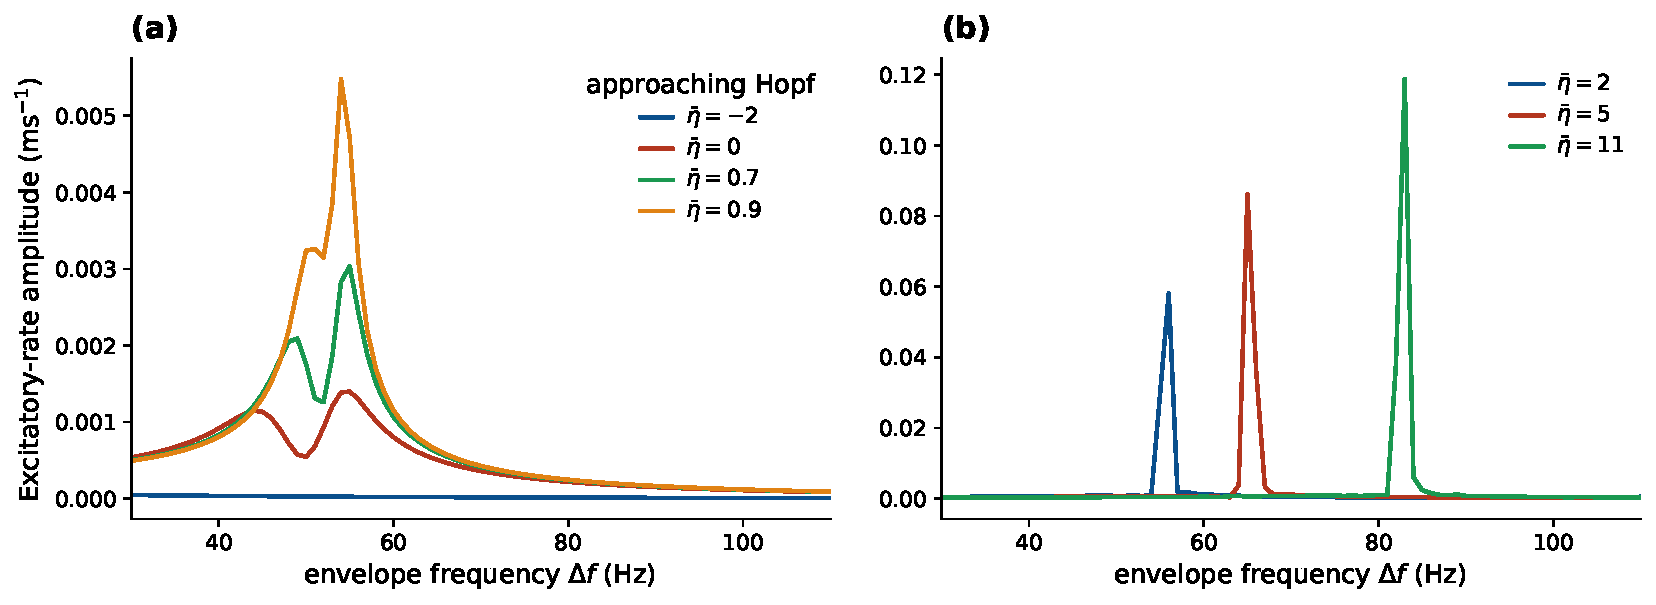
\includegraphics[width=\textwidth]{fig_nmm2_resonance_twotone.pdf}
\caption{\DIFdelbeginFL \DIFdelFL{\textbf{NMM2 PING gamma resonance (exact mean field, genuine two tones).}
Lock-in response of the excitatory rate $r_E$ at the envelope frequency $\Delta f$ }\DIFdelendFL \DIFaddbeginFL \DIFaddFL{\textbf{Gamma resonance in the PING mean field.}
Excitatory-rate lock-in }\DIFaddendFL under \DIFdelbeginFL \DIFdelFL{a
}\DIFdelendFL \DIFaddbeginFL \DIFaddFL{genuine }\DIFaddendFL two-tone \DIFdelbeginFL \DIFdelFL{TI field (}\DIFdelendFL \DIFaddbeginFL \DIFaddFL{input, }\DIFaddendFL carrier $300$~Hz\DIFdelbeginFL \DIFdelFL{)}\DIFdelendFL .
\emph{(a)} \DIFdelbeginFL \DIFdelFL{(stable focus}\DIFdelendFL \DIFaddbeginFL \DIFaddFL{Below $\bar\eta_H=1.110$}\DIFaddendFL , \DIFdelbeginFL \DIFdelFL{$\bar\eta<\bar\eta_H=1.110$) forced resonance at the gamma frequency
($f_0\!\approx\!54$}\DIFdelendFL \DIFaddbeginFL \DIFaddFL{forced-resonance peaks near
$f_0\approx54$}\DIFaddendFL ~Hz \DIFdelbeginFL \DIFdelFL{), the peak growing $0.0014\!\to\!0.0030\!\to\!0.0055$}\DIFdelendFL \DIFaddbeginFL \DIFaddFL{grow from $0.0014$ to $0.0030$ to $0.0055$}\DIFaddendFL ~ms$^{-1}$
\DIFdelbeginFL \DIFdelFL{as }\DIFdelendFL \DIFaddbeginFL \DIFaddFL{toward }\DIFaddendFL the Hopf\DIFdelbeginFL \DIFdelFL{is approached ($1/\gamma$ gain)}\DIFdelendFL . \emph{(b)} \DIFdelbeginFL \DIFdelFL{(limit cycle}\DIFdelendFL \DIFaddbeginFL \DIFaddFL{Above it}\DIFaddendFL , \DIFdelbeginFL \DIFdelFL{$\bar\eta>\bar\eta_H$) response }\DIFdelendFL \DIFaddbeginFL \DIFaddFL{peaks }\DIFaddendFL in the autonomous-gamma regime
\DIFdelbeginFL \DIFdelFL{, the peak shifting
upward with $\bar\eta$ ($56\!\to\!65\!\to\!83$}\DIFdelendFL \DIFaddbeginFL \DIFaddFL{shift from $56$ to $65$ to $83$}\DIFaddendFL ~Hz \DIFdelbeginFL \DIFdelFL{)}\DIFdelendFL \DIFaddbeginFL \DIFaddFL{with increasing $\bar\eta$}\DIFaddendFL .
The \DIFdelbeginFL \DIFdelFL{input carries no power at
$\Delta f$; the response is synthesized by the exact quadratic $v^2$ }\DIFdelendFL \DIFaddbeginFL \DIFaddFL{voltage }\DIFaddendFL nonlinearity \DIFdelbeginFL \DIFdelFL{, with no
sigmoid anywhere in }\DIFdelendFL \DIFaddbeginFL \DIFaddFL{$v^2$ generates }\DIFaddendFL the \DIFdelbeginFL \DIFdelFL{model}\DIFdelendFL \DIFaddbeginFL \DIFaddFL{beat absent from the input}\DIFaddendFL .
AM/two-tone comparisons are \DIFdelbeginFL \DIFdelFL{reported }\DIFdelendFL in the supplement (\S\ref{supp:waveform-checks}).}
\label{fig:nmm2_res}
\end{figure}

\begin{figure}[t!]
\centering
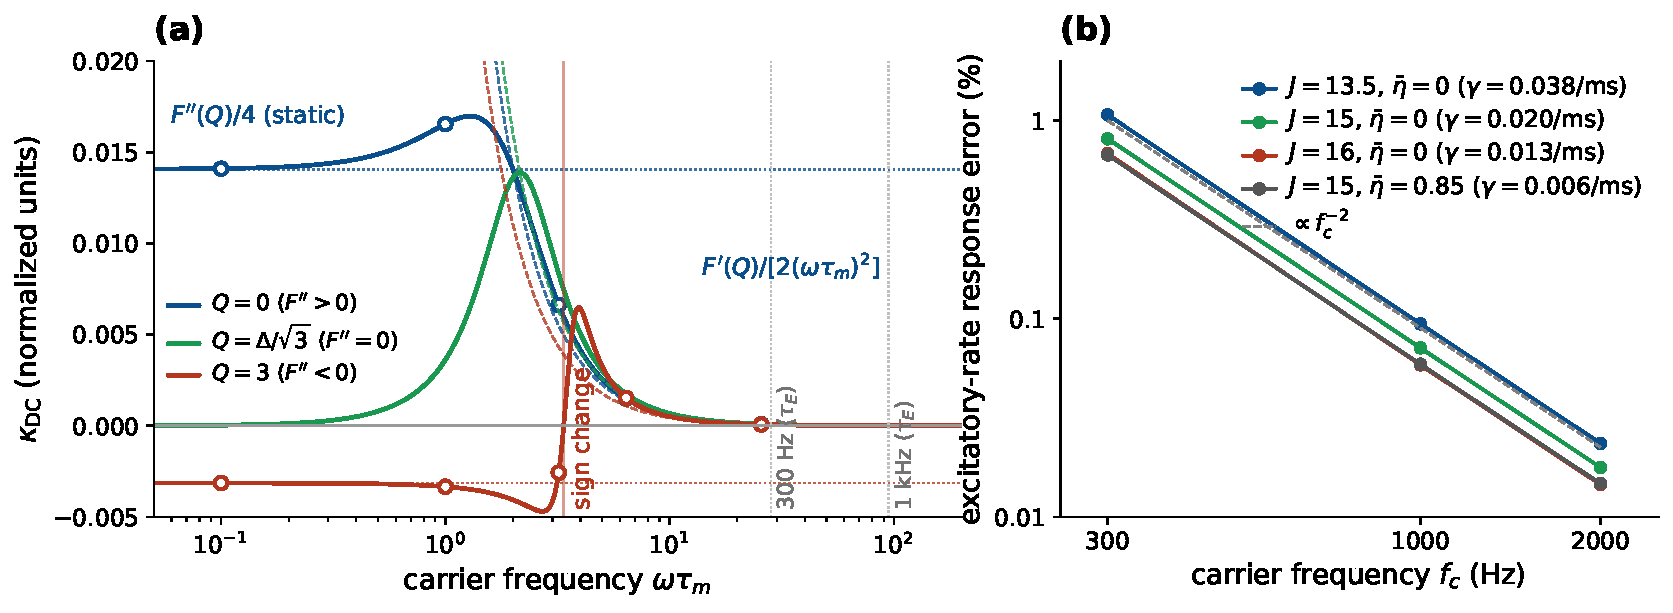
\includegraphics[width=\textwidth]{fig_mpr_crossover.pdf}
\caption{\textbf{Static curvature at slow carriers, slope at fast ones.} \emph{(a)}
Second-order DC rate shift of an uncoupled MPR population ($\Delta=1$) under a
current carrier, Eq.~\eqref{eq:crossover}, for operating points below, at and above the
inflection of $F(Q)$. Dotted: the static limit $\tfrac14F''$; dashed: the fast-carrier
limit $F'/[2(\omega\tau_m)^2]$; circles: RK4 integrations at $I_{\rm ac}=0.05$ averaged over whole carrier
periods (relative error below $10^{-3}$). Above the inflection the sign changes with carrier frequency. The horizontal coordinate is $\omega\tau_m$; the carrier markers
use $\tau_m=\tau_E=15$~ms. \emph{(b)} PING of Eq.~\eqref{eq:nmm2-ping}: relative error of the
fast-carrier difference-frequency source against the exact second-order response at four
stable operating points ($\gamma$ the damping of the gamma mode), two tones centered at
$300$, $1000$ and $2000$~Hz.}
\label{fig:crossover}
\end{figure}

\DIFaddbegin \DIFadd{The unpinned PING coupling sweep also approaches a gamma Hopf, but two
modes compete for the response peak. Near the Hopf, the critical mode's
linear gain has a fitted damping exponent of $1.02$; the full-sweep exponent
is $0.71$. At finite amplitude the response departs from the linear
reference and saturates, while the driven endpoint remains attracting.
The mode tracking, amplitude checks, and their numerical ranges accompany
the coupling curve in the supplement (\S\ref{supp:ping-coupling-results}).
Thus JR and PING share the critical mode's $1/\gamma$ gain law despite
their different detectors; the law does not describe every mode or the
entire finite-amplitude sweep.
}

\ifjne\else
\subsection{\DIFadd{Mode competition and finite-amplitude gain in PING}}\label{supp:ping-coupling-results}
\DIFaddend In NMM2 PING, $J$ is the mean inter-neuron QIF synaptic weight.
Sweeping $J$ at fixed background drive toward the gamma Hopf reveals two
competing modes (Fig.~\ref{fig:nmm2_jcurve}). A second mode near $55$~Hz carries
the linear-response peak over $14.6\lesssim J\lesssim16.2$; the critical mode
carries it at lower couplings and again near the Hopf, where its frequency is
about $50$~Hz. In that near-Hopf interval,
$0.0014\lesssim\gamma\lesssim0.0081$~ms$^{-1}$, the linear gain scales as
$1/\gamma$ with a fitted exponent of $1.02$ over a $5.8$-fold damping range.
The full-sweep exponent is $0.71$, so a single-mode law does not describe the
whole curve. Coupling-dependent sensitivity \cite{clusella2023} therefore
includes changes in which mode carries the peak.

At $A_f=8$, the simulated response exceeds the normalized linear reference by
up to $48\%$ in the amplitude check, then saturates. At a quarter of that
amplitude ($A_f=2$, one sixteenth of the power), the departures stay within
$11\%$ at the nine tested couplings. The driven endpoint remains attracting under both waveforms
(\DIFdelbegin \DIFdel{supplement, }\DIFdelend \S\ref{app:ping-stability}).
The alpha JR and gamma NMM2 circuits share the $1/\gamma$ gain scaling of their critical mode despite their different
mixers, with amplification adjustable through coupling.

\DIFaddbegin \fi

\DIFaddend \subsection{QIF responses distinguish beat modulation from field-induced gamma}\label{sec:qif}
\DIFdelbegin \DIFdel{Below the field-induced Hopf, the }\DIFdelend \DIFaddbegin \DIFadd{The finite }\DIFaddend QIF network shows beat-locked modulation \DIFdelbegin \DIFdel{with
a small mean-rate change; above it, the field induces gamma and adds a beat
component. The }\DIFdelend \DIFaddbegin \DIFadd{at the lower tested
amplitude and field-induced gamma at the higher amplitude. Its }\DIFaddend $8000$-neuron populations test
\DIFdelbegin \DIFdel{this distinction }\DIFdelend \DIFaddbegin \DIFadd{these regimes }\DIFaddend at the spike level
\cite{montbrio2015,ruffini2025rosetta,clusella2023}
(Figs.~\ref{fig:qif_raster},~\ref{fig:qif_regimes}).

\DIFdelbegin \DIFdel{An unmodulated carrier matched in RMS input current (model units)
provides this control in the mean field (Fig.~\ref{fig:qif_regimes}c,d). It produces a rectified E-drive
shift within $3\%$ of TI's and a similar mean-rate increase. At $A_f=35$, both
waveforms induce gamma near $51$~Hz, whereas TI also produces the $55$~Hz beat
component. At }\DIFdelend \DIFaddbegin \DIFadd{At $\bar\eta=0.85$ and }\DIFaddend $A_f=10$\DIFdelbegin \DIFdel{, neither induces gamma, and TI alone produces a resolved beat
response. A longer window reduces the single carrier's apparent $55$~Hz
depth from $0.011$ to $9.2\times10^{-5}$, while TI's stays at $0.30$--$0.31$;
the former is spectral leakage. The equal-RMS control separates induction
of gamma from the beat response and has been tested only in the mean field.
}%DIFDELCMD <

%DIFDELCMD < %%%
\DIFdel{The $A_f=35$ runs are finite-amplitude illustrations: the fast-carrier voltage
excursion is about $1.2$ per tone in model units. At $A_f=10$}\DIFdelend , the estimated rectified E-drive shift
is $0.12$, below the E-only Hopf threshold $\delta\eta_E^*\approx0.286$\DIFdelbegin \DIFdel{; the stronger drive exceeds it, as quantified below.
}%DIFDELCMD <

%DIFDELCMD < %%%
\DIFdel{At $\bar\eta=0.85$ and $A_f=10$, beat depths span about }\DIFdelend \DIFaddbegin \DIFadd{.
Beat depths span }\DIFaddend $0.09$--$0.16$ across cutoff and population choices,
\DIFdelbegin \DIFdel{versus }\DIFdelend \DIFaddbegin \DIFadd{compared with }\DIFaddend $0.13$ in the mean field. \DIFdelbegin \DIFdel{The }\DIFdelend \DIFaddbegin \DIFadd{Population doubling changes the
}\DIFaddend cutoff-free \DIFdelbegin \DIFdel{theta form gives $0.156$ at $N=8000$ and $0.137$ at
$N=16000$, a }\DIFdelend \DIFaddbegin \DIFadd{depth by }\DIFaddend $12\%$\DIFdelbegin \DIFdel{change exceeding the pilot tolerance. The baseline
mean-rate increase is $2.8\%$, but the modulation's size is not converged
}\DIFdelend \DIFaddbegin \DIFadd{, so its quantitative size remains unconverged
}\DIFaddend (supplement, \S\ref{supp:theta-pilot})\DIFaddbegin \DIFadd{; the baseline mean-rate increase is
$2.8\%$}\DIFaddend . At $\bar\eta=1.5$, the original finite-cutoff run gives a
$42$~Hz depth of about $0.02$ and a $1.6\%$ mean-rate increase\DIFdelbegin \DIFdel{; }\DIFdelend \DIFaddbegin \DIFadd{, while
}\DIFaddend ongoing gamma dominates.

At \DIFdelbegin \DIFdel{the larger amplitude }\DIFdelend $A_f=35$ and $\bar\eta=0.85$, \DIFdelbegin \DIFdel{stimulation produces
a dominant }\DIFdelend \DIFaddbegin \DIFadd{a }\DIFaddend line near $52$~Hz \DIFdelbegin \DIFdel{, with modulation depth about }\DIFdelend \DIFaddbegin \DIFadd{dominates
(depth }\DIFaddend $0.70$\DIFdelbegin \DIFdel{, and a smaller component
at }\DIFdelend \DIFaddbegin \DIFadd{), alongside }\DIFaddend the $55$~Hz beat \DIFdelbegin \DIFdel{, with }\DIFdelend \DIFaddbegin \DIFadd{(}\DIFaddend depth $0.29$\DIFdelbegin \DIFdel{. The second-order carrier-averaged system
predicts an excitatory }\DIFdelend \DIFaddbegin \DIFadd{). This is a
finite-amplitude example: the fast-carrier voltage excursion is about
$1.2$ per tone in model units. Carrier averaging predicts a }\DIFaddend drive shift
$\delta\eta_E\approx1.65$, beyond the E-only Hopf threshold\DIFdelbegin \DIFdel{$\delta\eta_E^*\approx0.286$, with }\DIFdelend \DIFaddbegin \DIFadd{, and }\DIFaddend a
leading eigenvalue \DIFdelbegin \DIFdel{whose real part is }\DIFdelend \DIFaddbegin \DIFadd{with real part }\DIFaddend $+0.032$~ms$^{-1}$. Direct mean-field
integration reproduces the off-beat line, \DIFdelbegin \DIFdel{supporting the interpretation of panel~(b) }\DIFdelend \DIFaddbegin \DIFadd{identifying the dominant
response }\DIFaddend as field-induced gamma \DIFdelbegin \DIFdel{with a
smaller forced component.}\DIFdelend \DIFaddbegin \DIFadd{(Fig.~\ref{fig:qif_raster}b).
}\DIFaddend

\DIFdelbegin %DIFDELCMD < \begin{figure}[t!]
%DIFDELCMD < \centering
%DIFDELCMD < 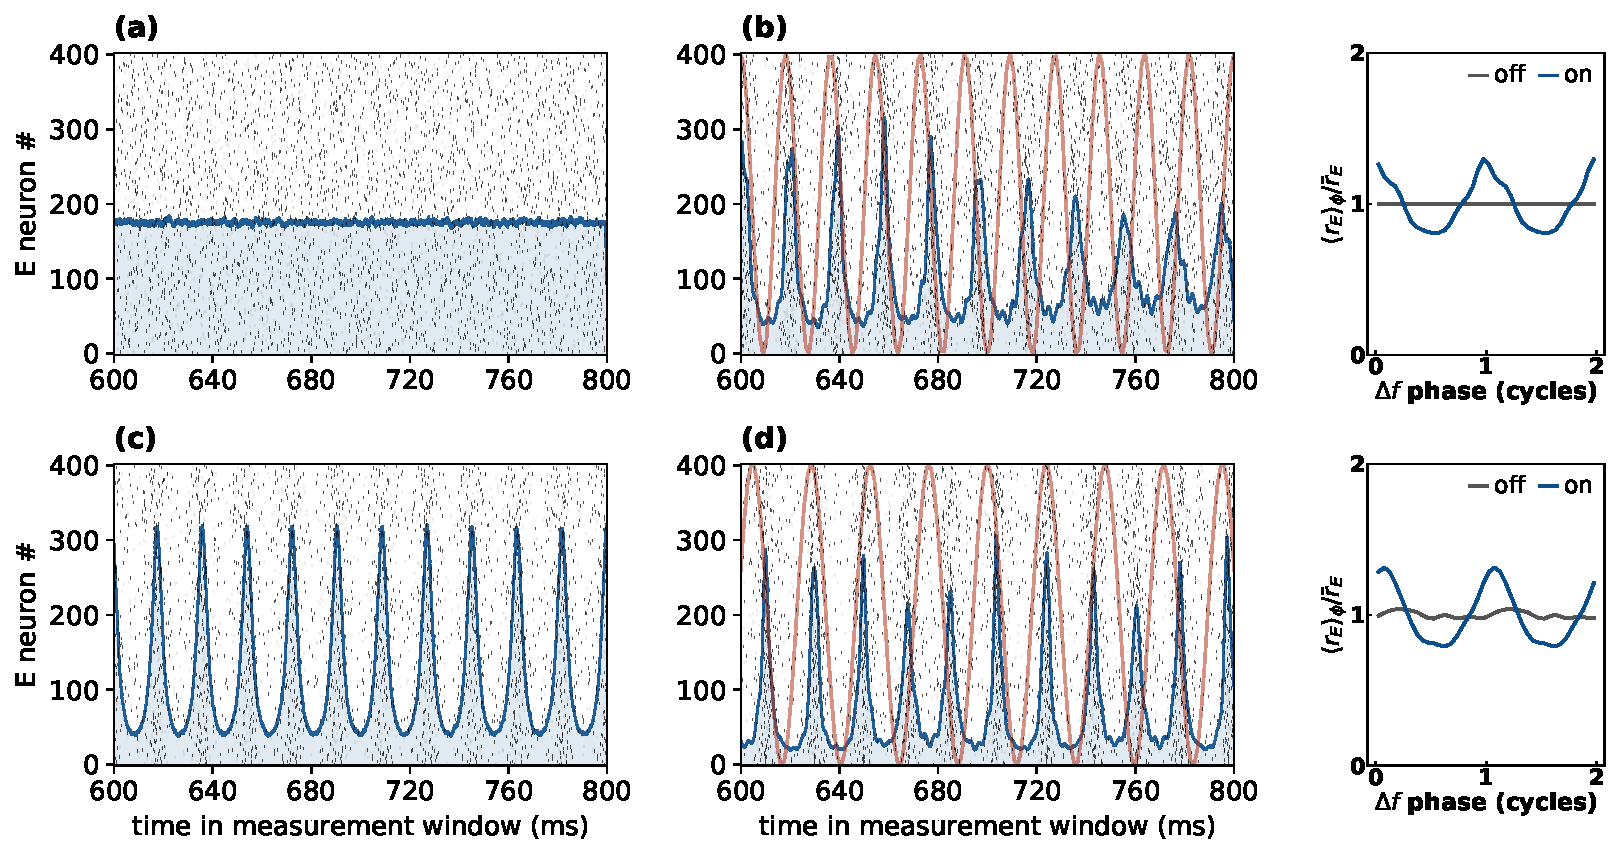
\includegraphics[width=\textwidth]{fig_qif_raster_twotone.pdf}
%DIFDELCMD < %%%
%DIFDELCMD < \caption{%
{%DIFAUXCMD
\DIFdelFL{\textbf{Beat-locked activity superposed on gamma.}
QIF network, $N=8000$ per population, $A_f=35$ per tone, carrier $300$~Hz.
Black ticks: 400 E neurons; blue: smoothed rate on its own scale; red:
envelope in arbitrary units. The last $200$~ms are shown.
\emph{(a,b)} Field off/on at $\bar\eta=0.85$, beat $55$~Hz: induced gamma
near $52$~Hz dominates. \emph{(c,d)} Field off/on at $\bar\eta=1.5$,
beat $42$~Hz: autonomous gamma remains dominant.
Right-hand panels fold rate on beat phase over $44$ and $34$ cycles, respectively,
normalized to each condition's mean (off gray, on blue; scale 0--2).
Folding suppresses non-beat-locked gamma and exposes the smaller beat component;
it does not establish gamma-amplitude gating or phase capture.}}
%DIFAUXCMD
%DIFDELCMD < \label{fig:qif_raster}
%DIFDELCMD < \end{figure}
%DIFDELCMD <

%DIFDELCMD < \begin{figure}[t!]
%DIFDELCMD < \centering
%DIFDELCMD < 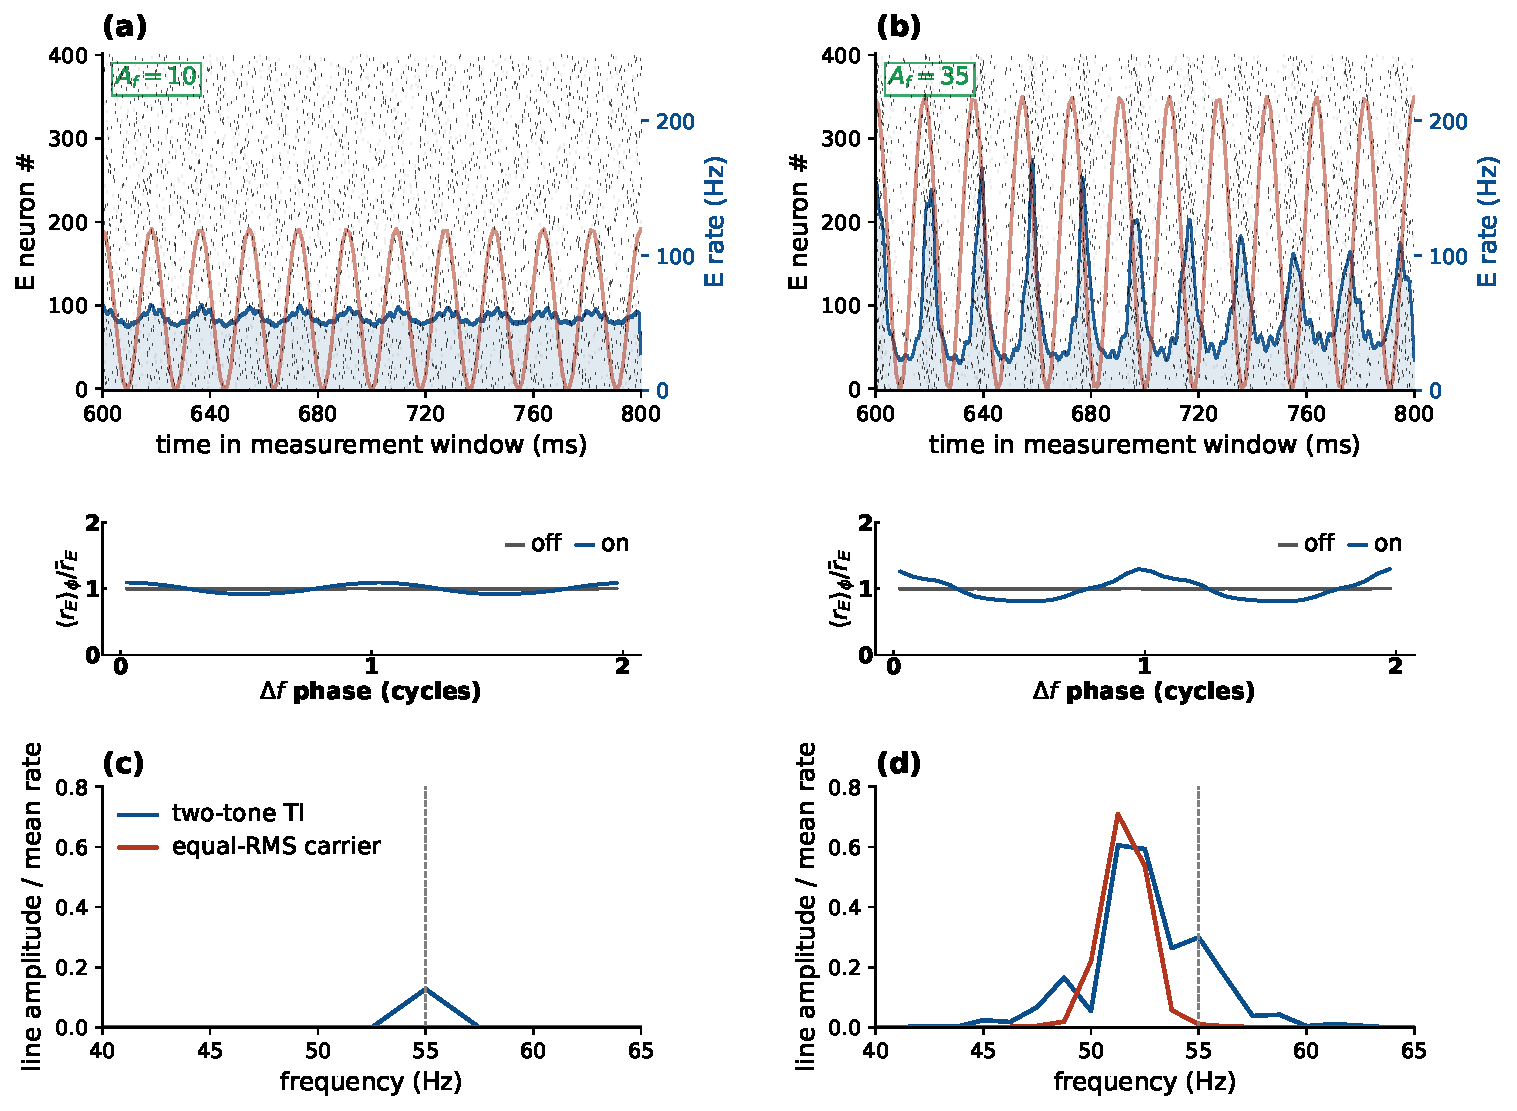
\includegraphics[width=\textwidth]{fig_qif_regimes.pdf}
%DIFDELCMD < %%%
%DIFDELCMD < \caption{%
{%DIFAUXCMD
\DIFdelFL{\textbf{TI and an equal-RMS carrier across the gamma threshold.}
Background $\bar\eta=0.85$, carrier $300$~Hz, beat $55$~Hz.
\emph{(a,b)} Spiking network at $A_f=10$ and $35$ per tone.
Black: 400 of 8000 E neurons; blue: population rate on a common scale;
red: envelope. Panels below the rasters show mean-normalized phase folds
(off gray, on blue).
Beat depths at this cutoff are about $0.09$ and $0.3$, with mean-rate increases of $2.8\%$
and $10.5\%$; the larger input also induces gamma.
\emph{(c,d)} Mean-field spectra under TI (blue) and one carrier of peak
amplitude $\sqrt2 A_f$ (red), normalized to mean rate. Both induce gamma
at the larger input; TI adds the $55$~Hz beat (dashed).
Hann windows span $800$~ms after $800$~ms settling.
Spiking panels use $V_{\rm peak}=100$; weak-drive depth depends on cutoff and population size.
RMS matching is of input current in model units, not physical power.}}
%DIFAUXCMD
%DIFDELCMD < \label{fig:qif_regimes}
%DIFDELCMD < \end{figure}
%DIFDELCMD <

%DIFDELCMD < %%%
\DIFdelend At $\bar\eta=1.5$, autonomous gamma near $53$--$54$~Hz remains about
four times larger than the $42$~Hz beat component \DIFdelbegin \DIFdel{with stimulation
(panel~}\DIFdelend \DIFaddbegin \DIFadd{(Fig.~\ref{fig:qif_raster}}\DIFaddend d).
Their coexistence produces slower burst-height variations. \DIFdelbegin \DIFdel{The beat-phase average suppresses non-beat-locked gamma and exposes
the smaller component; it does not show the full rate variation.
}%DIFDELCMD <

%DIFDELCMD < %%%
\DIFdel{The beat and ongoing gamma mix, as in endogenous amplitude modulation
\cite{ruffini2025ham}, producing }\DIFdelend \DIFaddbegin \DIFadd{Mixing produces
}\DIFaddend sidebands near $95$ and $11$~Hz\DIFdelbegin \DIFdel{(Fig.~\ref{fig:qif_timing}b), establishing }\DIFdelend \DIFaddbegin \DIFadd{, as in endogenous amplitude modulation
\cite{ruffini2025ham}; these establish }\DIFaddend nonlinear mixing without distinguishing
gamma-amplitude gating from phase modulation \DIFdelbegin \DIFdel{; field-free }\DIFdelend \DIFaddbegin \DIFadd{(Fig.~\ref{fig:qif_timing}b).
Field-free }\DIFaddend gamma frequencies agree between the \DIFdelbegin \DIFdel{spiking }\DIFdelend \DIFaddbegin \DIFadd{finite }\DIFaddend network and mean field
(\DIFdelbegin \DIFdel{panel~}\DIFdelend \DIFaddbegin \DIFadd{Fig.~\ref{fig:qif_timing}}\DIFaddend a).

\DIFaddbegin \begin{figure}[t!]
\centering
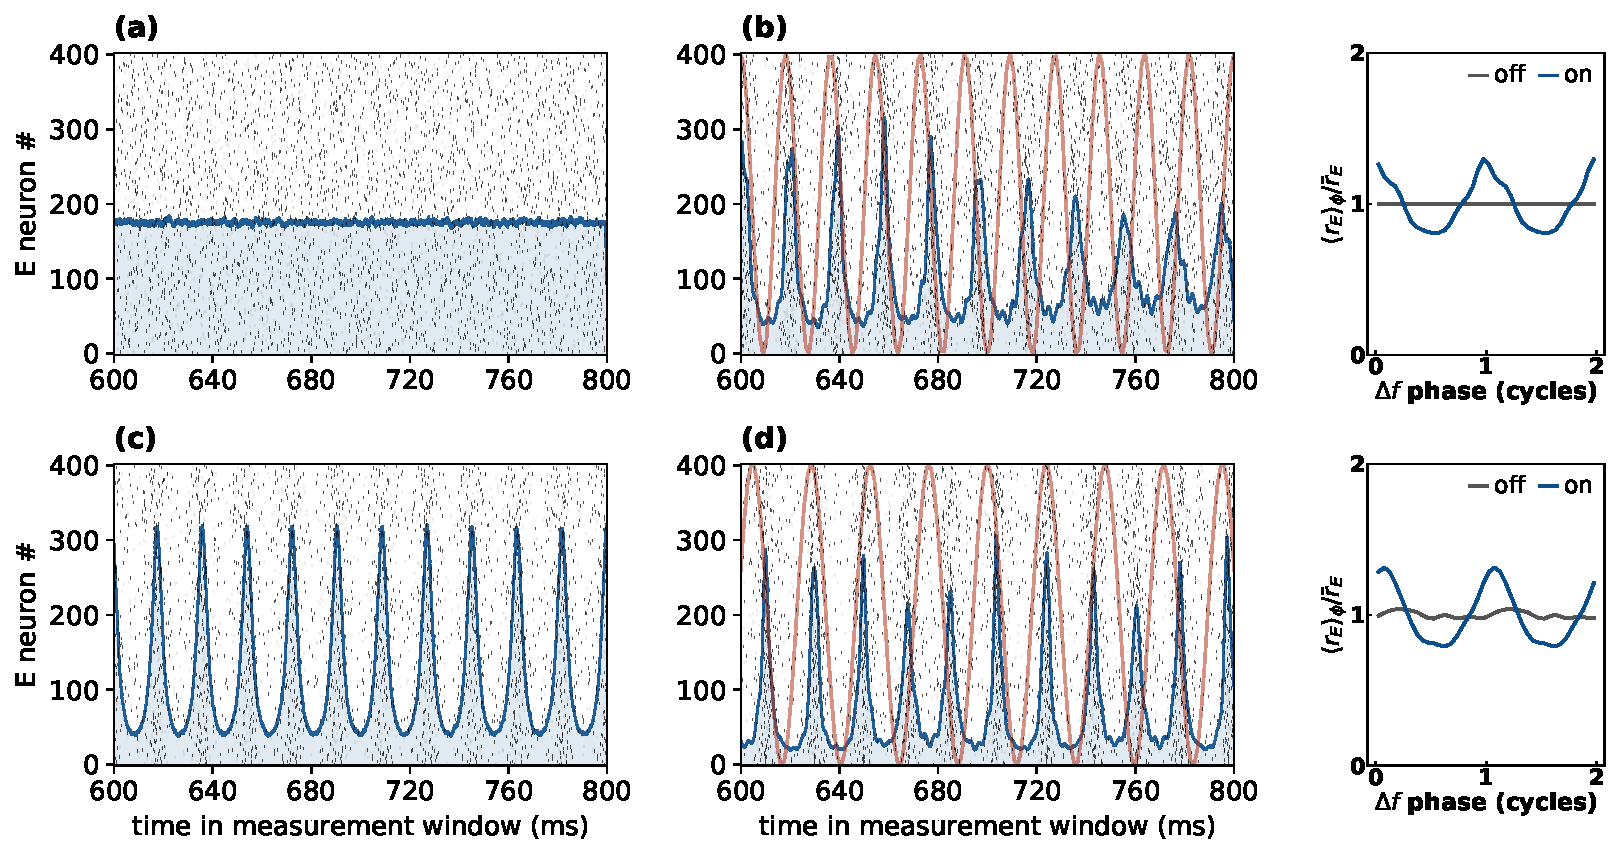
\includegraphics[width=\textwidth]{fig_qif_raster_twotone.pdf}
\caption{\DIFaddFL{\textbf{Beat-locked activity superposed on gamma.}
QIF network, $N=8000$ per population, $A_f=35$ per tone, carrier $300$~Hz.
Black ticks: 400 E neurons; blue: smoothed rate on its own scale; red:
envelope in arbitrary units. The last $200$~ms are shown.
\emph{(a,b)} Field off/on at $\bar\eta=0.85$, beat $55$~Hz: induced gamma
near $52$~Hz dominates. \emph{(c,d)} Field off/on at $\bar\eta=1.5$,
beat $42$~Hz: autonomous gamma remains dominant.
Right-hand panels fold rate on beat phase over $44$ and $34$ cycles, respectively,
normalized to each condition's mean (off gray, on blue; scale 0--2).
Folding suppresses non-beat-locked gamma and exposes the smaller beat component;
it does not establish gamma-amplitude gating or phase capture.}}
\label{fig:qif_raster}
\end{figure}

\DIFadd{To separate steady induction from beat-dependent activity, we compare TI
with an unmodulated carrier matched in RMS input current, in model units
(Fig.~\ref{fig:qif_regimes}c,d). In the mean field, their rectified E-drive
shifts agree within $3\%$ and their mean-rate increases are similar.
}\DIFaddend At $A_f=35$, \DIFaddbegin \DIFadd{both induce gamma near $51$~Hz; TI also produces the
$55$~Hz beat. At $A_f=10$, neither induces gamma, and TI alone produces
a resolved beat response. This control has been tested only in the mean
field; its spectral-leakage check is in the supplement
(\S\ref{supp:qif-protocol}).
}

\begin{figure}[t!]
\centering
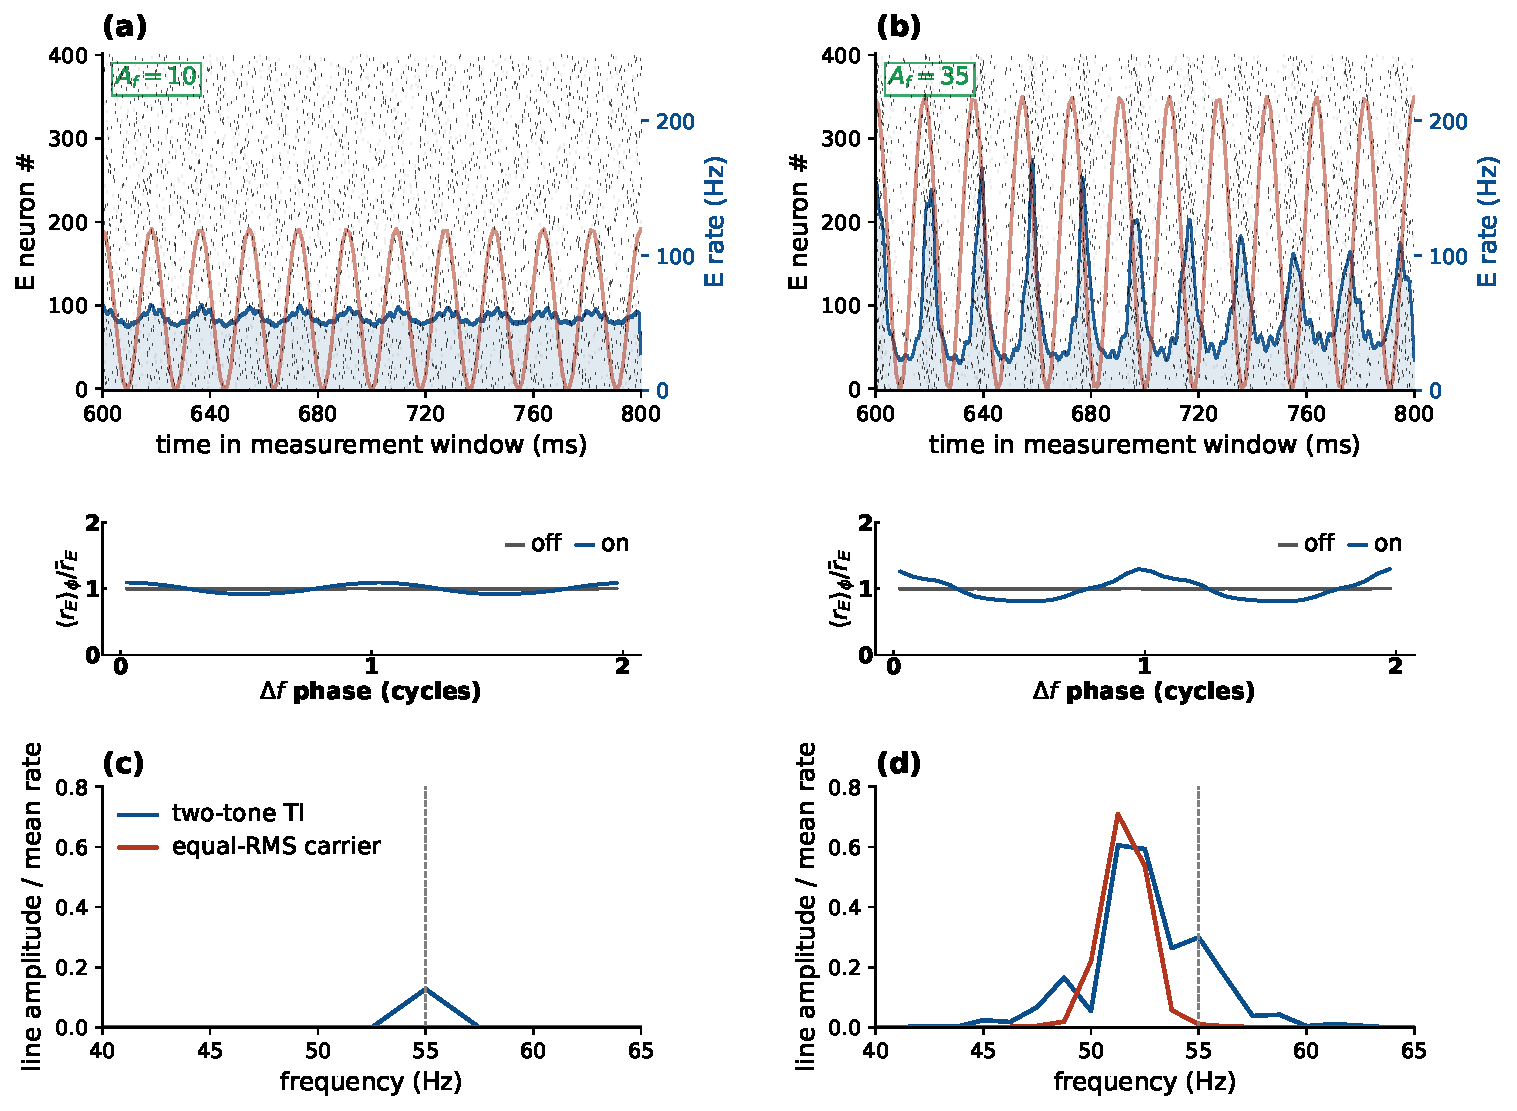
\includegraphics[width=\textwidth]{fig_qif_regimes.pdf}
\caption{\DIFaddFL{\textbf{TI and an equal-RMS carrier across the gamma threshold.}
Background $\bar\eta=0.85$, carrier $300$~Hz, beat $55$~Hz.
\emph{(a,b)} Spiking network at $A_f=10$ and $35$ per tone.
Black: 400 of 8000 E neurons; blue: population rate on a common scale;
red: envelope. Panels below the rasters show mean-normalized phase folds
(off gray, on blue).
Beat depths at this cutoff are about $0.09$ and $0.3$, with mean-rate increases of $2.8\%$
and $10.5\%$; the larger input also induces gamma.
\emph{(c,d)} Mean-field spectra under TI (blue) and one carrier of peak
amplitude $\sqrt2 A_f$ (red), normalized to mean rate. Both induce gamma
at the larger input; TI adds the $55$~Hz beat (dashed).
Hann windows span $800$~ms after $800$~ms settling.
Spiking panels use $V_{\rm peak}=100$; weak-drive depth depends on cutoff and population size.
RMS matching is of input current in model units, not physical power.}}
\label{fig:qif_regimes}
\end{figure}

\DIFadd{At $A_f=35$, population beat modulation exceeds the relative mean-rate
change by about threefold. Across }\DIFaddend the \DIFdelbegin \DIFdel{mean rate rises by about $8$--$11\%$ across the }\DIFdelend two conditions, \DIFdelbegin \DIFdel{while the beat modulation
depth , $A_\Omega/\langle r_E\rangle$, }\DIFdelend \DIFaddbegin \DIFadd{mean rate rises
$8$--$11\%$, while beat depth }\DIFaddend rises from below $0.003$ to $0.29$
($\bar\eta=0.85$) and $0.23$ ($\bar\eta=1.5$)
(Fig.~\ref{fig:qif_timing}c). \DIFdelbegin \DIFdel{Modulation is about three times the relative mean-rate change, but per-neuron
locking is weak: the }\DIFdelend \DIFaddbegin \DIFadd{Individual locking remains weak: median
}\DIFaddend pairwise phase consistency \DIFdelbegin \DIFdel{of single-neuron spike phases at
$\Delta f$ rises from its }\DIFdelend \DIFaddbegin \DIFadd{rises from $-0.02$ in the }\DIFaddend field-free control
\DIFdelbegin \DIFdel{(median $-0.02$) to a median of
}\DIFdelend \DIFaddbegin \DIFadd{to }\DIFaddend $0.003$--$0.005$, and \DIFdelbegin \DIFdel{the }\DIFdelend pooled vector strength from below $0.02$ to
$0.12$--$0.13$. \DIFdelbegin \DIFdel{The
population's beat-locked component is built from many }\DIFdelend \DIFaddbegin \DIFadd{Many }\DIFaddend weakly biased cells \DIFdelbegin \DIFdel{; these
}\DIFdelend \DIFaddbegin \DIFadd{therefore produce a population
beat component. These }\DIFaddend finite-amplitude \DIFdelbegin \DIFdel{runs }\DIFdelend \DIFaddbegin \DIFadd{results }\DIFaddend do not establish its size
under weak physiological stimulation.

\DIFaddbegin \FloatBarrier
\DIFaddend \section{Discussion}\label{sec:discussion}
\subsection{Cellular access and mixing require separate calibration}
The JR and QIF models \DIFdelbegin \DIFdel{separate mixing from recurrent
amplification, but neither
calibrates the full pathway from physiological kHz fields to a neural response}\DIFdelend \DIFaddbegin \DIFadd{demonstrate local mixing followed by recurrent
amplification. Applying these mechanisms to physiological kHz stimulation
requires calibration of membrane access and the generated source}\DIFaddend . The short-time
cases in Table~\ref{tab:doors} are access \DIFdelbegin \DIFdel{hypotheses with
preparation-dependent coupling; changing the QIF time constant tests sensitivity
to those assumptions}\DIFdelend \DIFaddbegin \DIFadd{assumptions; varying the effective
membrane time quantifies their consequences}\DIFaddend . Cellular mixing \cite{mirzakhalili2020,luff2024mixer} and network
amplification \cite{caldas2024,karimi2024,esmaeilpour2021} \DIFdelbegin \DIFdel{supply
complementary
evidence for the stages, not a joint calibration}\DIFdelend \DIFaddbegin \DIFadd{have complementary
experimental and modeling support; their combined transfer remains unmeasured}\DIFaddend .

At fields of order $1$~V/m, channels respond through membrane polarization,
well below fields associated with direct protein effects
\cite{cifra2026}.\footnote{That review describes direct effects at $10$~kV/m
to GV/m, depending on molecule and protocol; it excludes fields below
$0.1$~kV/m, where it expects direct effects to be negligible against thermal noise.}
Terminals can polarize more strongly than somata
\cite{rahman2013,aberra2023,chakraborty2018}. Small size alone does not imply
fast charging: specific membrane resistance times capacitance is area-independent;
conductance, geometry, and stimulation mode determine access. The supplementary
comparison distinguishes these mechanisms from strong-pulse charging
(\S\ref{supp:access}).
\ifjne\else
\subsection{Access assumptions in related models}
Short access times motivate the model but remain preparation-dependent.
The $1$ and $0.4$~ms cases of \cite{esmaeilpour2021} precede our effective-time
hypothesis. Luff et al.'s pulse-width-modulated TI model uses $1$~ms within a
$1$--$100$~ms passive-time sweep \cite{luff2024}. The $0.7~\mu$s charging
measured by Semenov et al.\ under strong microsecond field pulses
\cite{semenov2025} concerns a different response mode from intracellular
current charging or periaxonal conduction. A $10$--$100$-fold reduction in
QIF membrane time is therefore a sensitivity hypothesis, whose population
consequence follows from the slow-synapse limit.

\fi

Missey et al.\ \cite{missey2026} report biomarker suppression with both
low- and high-kHz carriers. Their Methods specify $1300/1430$~Hz at one
center and $9000/9130$~Hz at the other centers. For these pairs, the
$0.2$~ms point-membrane model predicts a high/low source ratio of $0.030$
at matched local fields. This comparison challenges that access hypothesis
but does not test it directly: carrier band was confounded with center,
local polarization was unmeasured, and a nonlinear or saturating physiological
readout could reconcile different sources with similar biomarker changes.

\subsection{Detector laws predict different spatial responses}
The head-model comparison separates geometric consequences of detector laws.
The product and summed-squares maps differ from the envelope map even before
state-dependent detection and network gain are applied. The fixed quadratic
pattern follows algebraically from fixed field shapes and linear access;
opposite envelope and mean-square centroid motion is a result for the tested
subject and montages, not a general steering law. A sharp rectifier can follow
the envelope over a finite amplitude range while smoothing or heterogeneity
restores quadratic behavior at smaller inputs. Amplitude and harmonic sweeps
therefore complement the spatial comparison.

The connection to Violante et al.\ \cite{violante2023} is a hypothesis generated
by these maps. Their models and cadaver recordings supported anterior envelope
steering from $2+2$~mA to $1+3$~mA. During participants' 32~s encoding blocks,
1:3 reduced the evoked blood-oxygen-level-dependent (BOLD) response relative
to sham ($P=0.006$) and 1:1 ($P=0.015$); 1:1 did not differ from sham
($P=0.953$). The stimulation-by-region interaction was nonsignificant
($P=0.76$), so the physiology did not establish spatial steering. Significant
voxelwise reductions extended beyond the anterior focus: 30\% of anterior,
25\% of posterior, and 2\% of middle hippocampal voxels.

In IXI002, mean-square polarization rises by 24\% under 1:3, while mean
envelope excursion falls by 45\% and both quadratic beat maps fall by 25\%.
At fixed uniform static curvature the steady-source magnitude therefore rises
by 24\%; a mean shift from rectification of the beat instead scales as
$(3/4)^2\approx0.56$ in the weak-response limit. The first ordering is
consistent with stronger BOLD suppression if the steady source lowers activity
and the hemodynamic response preserves that ordering. A slow linear readout
suppresses a zero-mean $5$~Hz beat while retaining a shift over the stimulation
window; nonlinear neural or vascular responses can also convert that beat into
a mean change or alter the encoding response.

This comparison does not identify the biological detector. Local envelope excursion can \DIFaddbegin \DIFadd{also }\DIFaddend increase under 1:3
\DIFdelbegin \DIFdel{where $|\mathcal P_1|>2|\mathcal P_2|$,
reaching $1.5\times$ where $|\mathcal P_1|\geq3|\mathcal P_2|$ }\DIFdelend (supplement, \S\ref{supp:steering-algebra})\DIFdelbegin \DIFdel{; }\DIFdelend \DIFaddbegin \DIFadd{, allowing }\DIFaddend a selective or
thresholded envelope response\DIFdelbegin \DIFdel{remains possible}\DIFdelend . Equal summed currents do not match local RMS polarization,
and the nonsignificant 1:1--sham result does not establish a null effect.
Heterogeneous curvature and unknown recurrent and hemodynamic gains can change
the predicted ordering. Measuring spatially resolved steady and beat responses
at controlled polarization and state, with an equal-RMS carrier control,
would discriminate the hypotheses.
\ifjne\else
\subsection{\DIFdelbegin \DIFdel{Mean-square change }\DIFdelend \DIFaddbegin \DIFadd{Envelope and mean-square changes }\DIFaddend under current-ratio steering}\label{supp:steering-algebra}
The mean-square polarization
changes by $\mathcal I_{1:3}/\mathcal I_{1:1}
=(\mathcal P_1^2+9\mathcal P_2^2)/[4(\mathcal P_1^2+\mathcal P_2^2)]$,
exceeding one only where $|\mathcal P_2|>\sqrt{3/5}|\mathcal P_1|
\approx0.775|\mathcal P_1|$. Its hippocampal mean rises by 24\% and its focus
moves 4.5~mm posteriorly. Equal summed currents therefore do not match local
RMS polarization.

\DIFaddbegin \DIFadd{Local envelope excursion increases under 1:3 where
$|\mathcal P_1|>2|\mathcal P_2|$, reaching $1.5\times$ where
$|\mathcal P_1|\geq3|\mathcal P_2|$. A selective or thresholded envelope
response therefore remains possible despite the lower ROI mean excursion.
}

\DIFaddend \fi

\subsection{Field-induced oscillations and resonant amplification}
At stronger fields, TI and unmodulated carriers can have similar excitation
thresholds \cite{opancar2025,semenov2025}, and peripheral responses need not
extract the envelope \cite{peripheral2023}. Our weak-input calculation concerns
modulation of ongoing activity \cite{vieira2024}; the finite-amplitude
QIF examples instead show a mean shift crossing a circuit Hopf. That boundary
depends on amplitude and initial state, and supplies no physiological threshold.
The supplementary laminar extension tests two resonant bands at low carriers
(\S\ref{app:lanmm}), outside TI's kHz regime.

The common TI/tACS amplifier follows from matching source, readout, and state,
consistent with excitatory--inhibitory models \cite{ledoux2011,clusella2023}
and related tACS/AM phase-locking studies
\cite{ali2013,negahbani2018,krause2023}. Stimulation-induced state shifts can
change the finite-amplitude ratio. Near-Hopf temporal slowing does not by itself
establish a diverging spatial correlation length. \DIFdelbegin \DIFdel{Writing the reverberation time
as }\DIFdelend \DIFaddbegin \DIFadd{With reverberation time
}\DIFaddend $\tau_{\rm rev}=1/\gamma$, the quality factor is $\mathcal Q=\pi f_0\tau_{\rm rev}$
and power bandwidth approximately $1/(\pi\tau_{\rm rev})$.
Relaxation over a few hundred milliseconds \cite{wilting2018} gives
order-ten quality and order-$1$~Hz bandwidth at $10$~Hz, making detuning
consequential; that measured relaxation is not specific to an alpha mode.

\subsection{Efficiency depends on the generated drive}
Measured DC couplings are $0.12$--$0.18$~mV per V/m in hippocampus
($0.21$ at $10$~Hz) \cite{bikson2004,deans2007} and reach $0.5$~mV per V/m
in cortical L5/6 pyramidal cells \cite{radman2009}; human cortical fields near
$0.8$~V/m have been reported at $2$~mA \cite{huang2017,huang2017corr}.
These measurements constrain illustrative input budgets, not the kHz transfer.
The $2$--$5\%$ source comparison in \S\ref{sec:direct-comparison} matches
each TI carrier's polarization to the direct input. Matching the total TI
peak instead halves the ratio to
$\mathcal R_{\rm det}\simeq|\Sig''|\varepsilon/(4\Sig')$; common recurrent
gain cancels in linear response.

For $E_j=0.5$~V/m, $\lambda_0=0.5$~mV per V/m, $f_c=2$~kHz and the assumed
$\tau_m=0.2$~ms, access gives $\varepsilon\approx0.092$~mV. Rounding to
$0.1$~mV yields $\mathcal R_{\rm det}\approx0.8\%$ at $v^*=8.30$~mV
under total-peak matching. This is an assumed input budget, not an inferred
polarization in recorded cells.

For comparison, the carrier-averaged, matched-peak, open-loop ratio has a
numerically estimated supremum of $0.348$ over bounded nondecreasing memoryless
transfers (supplement, \S\ref{app:bound}, Eq.~\eqref{eq:etasup}). A positive
mixture of step responses extends the logistic calculation to this class.
Approaching the bound requires a transition sharp relative to the input:
microvolt logistic widths at the illustrative polarizations. Its step-like
limit has a second-harmonic ratio near $0.15$, differing from weak square-law
and linear envelope detection. The bound excludes dynamic QIF and general
cellular mechanisms. Increasing a common matched polarization cannot exceed
it; unequal polarizations invalidate the matching. Unequal-current TI and
matched-depth AM-tACS comparisons do not measure this open-loop ratio.

Vieira et al.'s weaker TI effects \cite{vieira2024} are compatible with a
smaller beat source, but their local mixer polarizations were unmatched
(supplement, \S\ref{supp:vieira}). Phase-locking value (PLV) also depends on
baseline and state. A calibrated amplitude sweep with a common readout is
needed to estimate the detector coefficient.

\subsection{Limits of the population description}
Synaptic filters before a detector further attenuate its input. Model choice
also matters: Hodgkin--Huxley and Frankenhaeuser--Huxley models reproduce
stimulus-evoked firing missed by the tested leaky, exponential, and
adaptive-exponential integrate-and-fire models \cite{plovie2025}.
Noise, additional heterogeneity, and intercolumn interactions can broaden or
shift our deterministic resonances. Human findings include peripheral effects
without central effects \cite{iszak2023} and null occipito-parietal alpha-power
modulation \cite{mansourinezhad2025}. Access, generated sources, and circuit
tuning therefore need measurement in the same preparation.

\subsection{Falsifiable predictions and tests}\label{sec:predictions}
Table~\ref{tab:predictions} \DIFdelbegin \DIFdel{separates tests of access, detection, and amplification
from observations already consistent with the model. Quantitative reanalysis of
the }\DIFdelend \DIFaddbegin \DIFadd{distinguishes the measurements needed to test each
stage. Interpreting }\DIFaddend timing and synaptic-blockade data requires \DIFdelbegin \DIFdel{the amplitude and harmonic controls
of \S\ref{sec:transduction-methods}, with detector and network changes measured
separately}\DIFdelend \DIFaddbegin \DIFadd{independent
measurements of amplitude scaling, harmonic content, and recurrent gain}\DIFaddend .

Network filtering must be separated from the harmonic signature. At resonance
with $\mathcal Q=10$, a detector ratio of $20\%$ appears as only $0.7\%$,
which could make an envelope follower look quadratic. Driving off resonance
at $\Delta f\simeq f_0/4$ places both harmonics on the flatter part of the
response, where $|G(2\Omega)/G(\Omega)|\approx1.22$--$1.25$ for
$\mathcal Q=3$--$30$. Alternatively, a weak direct tACS sweep can measure
$G$ independently so its effect can be removed from the harmonic ratio.

\begin{table}[htbp]
\centering\small
\renewcommand{\arraystretch}{1.15}
\begin{tabular}{@{}>{\raggedright\arraybackslash}p{0.30\textwidth}
 >{\raggedright\arraybackslash}p{0.64\textwidth}@{}}
\toprule
Model prediction & Discriminating measurement \\
\midrule
Access and detector dynamics & Sweep carrier frequency and tonic state at fixed
beat. Measure local polarization and network gain separately; normalize the
beat source by the carrier product and compare its magnitude and phase. \\[4pt]
Quadratic versus envelope detection & Vary carrier amplitudes independently,
then together. A weak quadratic source follows their product; an envelope
follower follows the minimum. Measure amplitude scaling and harmonics off
resonance or correct their network gains; a single harmonic ratio is insufficient. \\[4pt]
Fixed quadratic spatial pattern & Vary the current ratio at fixed electrodes,
frequencies, and state. Compare normalized physiological beat maps with fixed
local orientations. Use a cortex-only reference for deep selectivity; measure
steady shifts and repeat at lower amplitude to test state changes. \\[4pt]
Resonant amplification & Sweep the beat through the intrinsic band across
states, measuring peak frequency, height, and width. A matched direct tACS
source tests the shared amplifier. \\[4pt]
Population modulation and mean response & Compare rate lock-in and mean shift
in the same units. Synaptic blockade tests recurrent amplification alongside
an independent cellular mixing measurement. Distinguish rate modulation from
single-neuron phase locking. \\[4pt]
Steady versus beat-dependent effects & Compare TI with an unmodulated carrier
of matched local RMS input and duration, checking the DC coefficient across
the carrier interval. Measure mean activity, intrinsic oscillations, and the
beat separately. \\
\bottomrule
\end{tabular}
\caption{Tests separating the proposed mechanisms. The detailed evidence matrix
and qualifications are in the supplement (\S\ref{supp:prediction-evidence}).
RMS matching refers to the detector input, not electrode or tissue power.}
\label{tab:predictions}
\end{table}

\DIFaddbegin \FloatBarrier
\DIFaddend \section{Conclusion}
\DIFdelbegin \DIFdel{TI requires access}\DIFdelend \DIFaddbegin \DIFadd{Access}\DIFaddend , detection, and amplification \DIFdelbegin \DIFdel{. For }\DIFdelend \DIFaddbegin \DIFadd{determine different parts of the TI response. With nonzero curvature, }\DIFaddend a weak static
scalar detector \DIFdelbegin \DIFdel{with nonzero curvature, detection }\DIFdelend generates a beat \DIFdelbegin \DIFdel{proportional
to the product of the local carrier polarizations }\DIFdelend \DIFaddbegin \DIFadd{weighted by the carrier-polarization product
}\DIFaddend and a steady source \DIFdelbegin \DIFdel{proportional to }\DIFdelend \DIFaddbegin \DIFadd{weighted by }\DIFaddend their summed squares. \DIFdelbegin \DIFdel{Dynamic QIF detection instead crosses
from curvature to positive-slope rectification as carrier frequency rises.
Fast axonal access can be represented
by a short effective membrane time, with its transfer still requiring calibration. }%DIFDELCMD <

%DIFDELCMD < %%%
\DIFdel{The detector law changes the spatial prediction. In the single-subject
geometric illustration, changing the current ratio moves the hippocampal
}\DIFdelend \DIFaddbegin \DIFadd{The steady sign depends on the detector: static JR
curvature and fast-carrier QIF dynamics can give opposite signs. At fixed
field shapes and neural state, current-ratio changes rescale the quadratic beat map; the opposite
}\DIFaddend envelope and mean-square \DIFdelbegin \DIFdel{centroids in opposite directions but only rescales the quadratic beat at fixed
neural state.
Under }\DIFdelend \DIFaddbegin \DIFadd{centroid shifts are specific to the head-model example.
With homogeneous conductivity and }\DIFaddend uniform scalar coupling and detection\DIFdelbegin \DIFdel{in homogeneous conductivity}\DIFdelend ,
the steady-source magnitude has no strict interior maximum.

Near a Hopf bifurcation, \DIFdelbegin \DIFdel{the circuit amplifies the beat in inverse proportion
to modal damping . TI shares this linear amplifier }\DIFdelend \DIFaddbegin \DIFadd{gain grows inversely with modal damping and is shared
}\DIFaddend with matched direct \DIFdelbegin \DIFdel{low-frequency stimulation}\DIFdelend \DIFaddbegin \DIFadd{tACS}\DIFaddend . In the pinned JR \DIFdelbegin \DIFdel{sweep, the response is expressed
mainly as beat-locked population-rate modulation; its ratio }\DIFdelend \DIFaddbegin \DIFadd{column it initially
favors beat modulation, while rectification of the amplified oscillation
increasingly contributes }\DIFaddend to the mean shift\DIFdelbegin \DIFdel{eventually falls
as the oscillation rectifies.
At larger fields, the }\DIFdelend \DIFaddbegin \DIFadd{.
At stronger drive, a }\DIFaddend steady shift alone can induce gamma, \DIFdelbegin \DIFdel{as can }\DIFdelend \DIFaddbegin \DIFadd{including under }\DIFaddend an
equal-RMS unmodulated carrier \DIFdelbegin \DIFdel{.
}%DIFDELCMD <

%DIFDELCMD < %%%
\DIFdelend \DIFaddbegin \DIFadd{in the mean field. Physiological kHz access remains
to be calibrated. }\DIFaddend Local-polarization measurements, independent-amplitude tests,
beat sweeps across states, and equal-RMS controls \DIFdelbegin \DIFdel{separate }\DIFdelend \DIFaddbegin \DIFadd{distinguish }\DIFaddend these mechanisms.
\DIFdelbegin \DIFdel{Together they test whether a measured TI response reflects access,
nonlinear detection, recurrent gain, or a field-induced change of state.
}\DIFdelend

\section*{Code and data availability}
Simulation code, cached results, and figure-generation scripts are provided at
\href{https://github.com/giulioruffini/TI-demodulation-paper}{the paper's GitHub repository};
the public archive is linked through
\href{https://doi.org/10.5281/zenodo.21009618}{Zenodo (doi:10.5281/zenodo.21009618)}.
The repository \texttt{README} maps figures to their scripts and distinguishes
recomputation from replotting cached data. The two-tone kHz example and both LaNMM carrier-measurement windows have
cached outputs and reproduction scripts. The FEM producer \texttt{code/fem\_quadmaps.py} computes the reported maps
and statistics from the stored fields; the summary arrays and
\texttt{code/make\_fem\_fig.py} reproduce Fig.~\ref{fig:fem} without the head model. Recomputing its maps
from the underlying fields currently requires Neuroelectrics' nonpublic
TI library and the original IXI002 fields and labels. A NumPy-only consumer,
\texttt{code/fem\_portable.py}, and an exporter with consistency checks are included;
the per-node export and its comparison with the published statistics remain
pending. Input hashes, settings, and export instructions are recorded in
\texttt{docs/fem\_ixi002\_violante.md}, \texttt{code/fem\_quadmaps.json},
and \texttt{docs/fem\_portable.md}.
The code in this paper's repository is released under CC-BY-4.0.
% Release hold: align the public repository/archive with this reviewed draft before submission.

\section*{Acknowledgments}
GR, BM, RS and FC have received funding from the European Research Council (ERC) under the
European Union's Horizon 2020 research and innovation programme (grant agreement No 855109,
GALVANI).
% RS support confirmed by Giulio via Klaus, 2026-10-19: GALVANI only.
% TODO before submission: funding for NG (Imperial), SC (IN, UMH-CSIC), and CM (IFISC, UIB-CSIC).
% IOP requires the funding agency AND grant number disclosed for all support.

\ifjne
\section*{Competing interests}
% Wording supplied by Giulio via Klaus, 2026-10-05; all authors confirm at submission.
% Shareholder wording follows the author-confirmed WP0215 journal declaration.
Giulio Ruffini, Ricardo Salvador, Borja Mercadal, and Francesca Castaldo are employees of
Neuroelectrics, which develops and sells transcranial electrical stimulation devices.
Giulio Ruffini is a co-founder and shareholder of Neuroelectrics. The other authors
declare no competing interests.

\section*{Author contributions}
% CRediT roles. Ricardo's roles confirmed by Giulio via Klaus, 2026-10-19.
% Remaining declarations need confirmation; all authors must approve the submitted version.
% Roles below reflect actual contributions; do not inflate them.
Using the CRediT taxonomy: \textbf{G.~Ruffini}: conceptualization, methodology, formal
analysis, software, investigation, visualization, writing (original draft), supervision,
funding acquisition. \textbf{R.~Salvador}: conceptualization (current-ratio steering),
methodology (head modeling), software, formal analysis, data curation, visualization.
\textbf{B.~Mercadal}: validation, visualization, writing (review and editing).
\textbf{R.~de Palma Aristides}: software, visualization, writing (review and editing).
\textbf{F.~Castaldo}: conceptualization, writing (review and editing).
\textbf{N.~Grossman}: conceptualization.
\textbf{S.~Canals}: supervision, writing (review and editing).
\textbf{C.~Mirasso}: supervision, writing (review and editing).
% TODO restore on sign-off: "All authors read and approved the final manuscript." (approval pending, 2026-09-22)
\fi

\section*{Declaration of generative AI and AI-assisted technologies in the manuscript
preparation process}
% IOP asks for the tool name and version, and expects prior drafts and prompts
% to be retained. TODO: pin the versions actually used before submission.
During the preparation of this work the authors used Anthropic Claude and OpenAI ChatGPT to
streamline the narrative and to assist with code and figure generation from data the authors
produced. The authors reviewed and edited all resulting content and take full responsibility
for the content of the published article.

\bibliographystyle{unsrt}
\bibliography{references}

\fi
% Article appendices are integral; additional material is routed by topic.
\clearpage
\appendix
\makeatletter
\let\ne@stdsection\section
\renewcommand{\section}{\clearpage\ne@stdsection}
\makeatother
\ifsupp
\section*{Notation and units}\phantomsection\label{app:notation-supp}
\def\notationtablelabel{tab:notation-supp}
% One notation source for the article, supplement, and full TN.
Table~\ref{\notationtablelabel} groups the symbols by their role in the calculation.
\ifappendices\else Symbols used only in supplementary derivations appear in the supplement's notation table.\fi
JR and LaNMM voltages are in mV and rates in s$^{-1}$. QIF voltages and current-like
drives are dimensionless model variables; QIF rates are physical rates, integrated
in ms$^{-1}$ and converted to Hz where indicated. The uncoupled MPR derivation explicitly uses membrane-time units; the main
population equations retain physical time and rate. All frequencies and time
constants in a formula must use the same time unit. In the FEM comparison $\mathbf n^*$ is the direction maximizing the envelope
at balanced currents, held fixed during the ratio sweep. A star otherwise marks a fixed point or,
on a bifurcation parameter, its critical value. Subscripts E and I identify
excitatory and inhibitory populations; they are not field or current variables.

\begingroup
\footnotesize
\setlength{\tabcolsep}{4pt}
\renewcommand{\arraystretch}{1.13}
\begin{longtable}{@{}>{\raggedright\arraybackslash}p{0.20\textwidth}
 >{\raggedright\arraybackslash}p{0.40\textwidth}
 >{\raggedright\arraybackslash}p{0.15\textwidth}
 >{\raggedright\arraybackslash}p{0.19\textwidth}@{}}
\caption{Notation and units. ``Normalized'' means dimensionless in the stated
model scaling; output units depend on the named observable. Equation numbers prefixed by S identify supplementary definitions; B-prefixed
numbers identify article-appendix equations, and unprefixed numbers identify
main-text equations. Lettered locations identify article appendices.}
\label{\notationtablelabel}\\
\toprule
Symbol & Meaning & Units & Defined in \\
\midrule
\endfirsthead
\multicolumn{4}{@{}l}{\textit{Table \thetable\ continued}}\\
\toprule
Symbol & Meaning & Units & Defined in \\
\midrule
\endhead
\midrule
\multicolumn{4}{r@{}}{\textit{Continued on next page}}\\
\endfoot
\bottomrule
\endlastfoot
\multicolumn{4}{@{}l}{\textbf{Field and access}}\\*
$E(t),E_0,\mathbf E_j$ & Applied field, its amplitude, and vector field of tone $j=1,2$ & V/m & Eq.~\eqref{eq:coupling} \\
$s(t),\varepsilon_j,\varepsilon$ & Local polarization; tone amplitudes; common amplitude ($\varepsilon_{\rm TI}$ and $\varepsilon_{\rm tACS}$ label the waveform) & mV & Eqs.~\eqref{eq:am}, \eqref{eq:doors} \\
$\varepsilon_{\rm D},\varepsilon_{\rm A},\varepsilon_{\rm eq}$ & Direct DC polarization, signed AC amplitude, and equivalent direct polarization matching a TI source & mV & \S\ref{sec:direct-comparison} \\
$I_j^{\rm pair},\mathcal P_j$ & Peak electrode-pair current; signed local polarization per unit current & mA; mV/mA & \S\ref{sec:envelope} \\
$\mathbf F_j,\sigma_{\rm cond}$ & FEM field per pair current; tissue conductivity & (V/m)/mA; S/m & \S\ref{sec:fem-methods} \\
$\mathcal A(t),\overline{\mathcal A}$ & Nonnegative polarization envelope and its beat-period mean & mV & Eq.~\eqref{eq:sqenv}; Table~\ref{tab:transduction-maps} \\
$f_1,f_2,f_c$ & Tone frequencies and their center & Hz & Eq.~\eqref{eq:am} \\
$\omega_j,\omega_c$ & Angular frequencies $2\pi f_j,2\pi f_c$ & rad/s & Eqs.~\eqref{eq:am}, \eqref{eq:doors} \\
$\Delta f,\Omega$ & Beat frequency $f_2-f_1$; $\Omega=2\pi\Delta f$ & Hz; rad/s & Eq.~\eqref{eq:am} \\
$m$ & AM-surrogate modulation depth & dimensionless & Eq.~\eqref{eq:amsur} \\
$\Lambda[E],\lambda_0,\lambda_f$ & Field-induced polarization; static and frequency-dependent coupling & mV; mV/(V/m) & Eqs.~\eqref{eq:nmm1}, \eqref{eq:doors} \\
$\boldsymbol\lambda^k_0,\boldsymbol\lambda^k_f$ & Coupling vectors for compartment $k$ & mV/(V/m) & Eq.~\eqref{eq:doors} \\
$H,H_k,H_m$ & Dominant-compartment access transfer, indexed transfer, and point-membrane transfer & dimensionless & Fig.~\ref{fig:models}; \S\ref{sec:coupling}, \S\ref{sec:khz} \\
$\tau_m,\tau$ & Membrane time; access-filter time in kHz controls & ms & Eqs.~\eqref{eq:mpr}, \eqref{eq:khz} \\
$f_{\rm char}$ & Characteristic frequency $1/(2\pi\tau)$ & Hz & Table~\ref{tab:doors} \\
\ifappendices
$\ell(\omega),\ell_0$ & Frequency-dependent and static cable space constants & $\mu$m & App.~\ref{app:access}, Eq.~\eqref{eq:lambda} \\
\fi
\ifappendices
$\mathbf V,\mathsf C_m,\mathsf G_m$ & Compartment voltages, capacitance and conductance matrices & V; F; S & App.~\ref{app:access} \\
\fi
\ifappendices
$\mathbf I^0,\mathbf p_E$ & Endogenous currents; field-to-current vector & A; A/(V/m) & App.~\ref{app:access} \\
\fi
$\mathbf x,\phi_j,\mathbf n$ & Position, field potential, unit cell orientation & m; V; unit vector & \S\ref{sec:envelope}, \S\ref{sec:dc} \\
$\mathcal I$ & Nonnegative mean-square local polarization before detector gain & mV$^2$ & \S\ref{sec:dc} \\
\addlinespace
\multicolumn{4}{@{}l}{\textbf{Detection}}\\*
$\Sig,\Sig',\Sig''$ & JR/LaNMM rate curve, slope and curvature & s$^{-1}$; s$^{-1}$mV$^{-1}$; s$^{-1}$mV$^{-2}$ & Eq.~\eqref{eq:sigmoid} \\
$e_0,v_0,\rho$ & Half the rate ceiling, inflection voltage, inverse voltage scale & s$^{-1}$; mV; mV$^{-1}$ & Eq.~\eqref{eq:sigmoid} \\
$\mathrm{PEIX}$ & Signed sigmoid saturation index & dimensionless & Eq.~\eqref{eq:peix} \\
$Y_\Omega,Y_{\rm DC}$ & Complex beat amplitude and signed steady source before recurrence & detector-output units & Eqs.~\eqref{eq:demod}, \eqref{eq:taylor} \\
$a_j^k,b_j^k,B_{kl}$ & Compartment polarization, polarization per current, bilinear mixing coefficient & mV; mV/mA; output/mV$^2$ & \S\ref{sec:envelope} \\
$\chi^{(2)}$ & Dynamic coefficient mapping a polarization product to a rate beat & s$^{-1}$mV$^{-2}$ & \S\ref{sec:coupling} \\
$g,T,Y_{\rm LF}$ & Memoryless response, envelope transduction, carrier-averaged output & specified output units & Eq.~\eqref{eq:cycavg} \\
$c_1,c_2,c_4$ & Linear, quadratic and quartic envelope coefficients & output/(mV)$^{1,2,4}$ & \S\ref{sec:transduction} \\
$\mathcal H_{\rm det},\mathcal H_{\rm meas}$ & Second/fundamental harmonic magnitude ratios before and after the network & dimensionless & Eq.~\eqref{eq:rdet} \\
$\mathcal M[y]$ & Peak-to-peak excursion of the quantity $y$ & units of $y$ & Eq.~\eqref{eq:reweight} \\
$F(Q),F',F''$ & MPR steady-rate curve and drive derivatives & normalized & Eq.~\eqref{eq:Fmpr} \\
$Q,q$ & Mean total drive $\bar\eta+I$; single-cell drive $\eta+I$ & normalized & Eq.~\eqref{eq:Fmpr}; App.~\ref{app:mpr-mixing} \\
$I_{\rm ac}$ & Single-tone current amplitude & normalized & \S\ref{sec:dynamic} \\
$\kappa_{\rm DC},\kappa_V$ & Mean-rate mixing per squared current or squared voltage excursion & normalized & Eqs.~\eqref{eq:crossover}, \eqref{eq:kfixed} \\
$d,\nu,\omega_z$ & MPR relaxation, ringing and zero-crossing angular frequencies & membrane-time units & App.~\ref{app:mpr-coefficients} \\
$\mathsf J,\mathbf h,H_v$ & Reduced MPR Jacobian, unit-current response and voltage transfer & normalized & \S\ref{sec:dynamic}; App.~\ref{app:mpr-mixing} \\
$\mathbf b_2,\mathsf I_2$ & Quadratic DC source per $I_{\rm ac}^2$; identity matrix & normalized & App.~\ref{app:mpr-mixing} \\
$\mathcal R_{\rm det},\mathcal R_{\rm lin}$ & TI/direct-drive source ratio; linear TI/tACS output ratio & dimensionless & App.~\ref{app:bound}; \S\ref{sec:tacs-results} \\
$\delta,\zeta$ & Threshold offset; sigmoid rate divided by $2e_0$ & mV; dimensionless & \S\ref{sec:transduction}; App.~\ref{app:bound} \\
\ifappendices
$u,\xi,\beta,k_{\rm ell}^2$ & Reduced amplitude $\rho\varepsilon$, offset $\rho(v^*-v_0)$, threshold ratio, elliptic parameter & dimensionless & App.~\ref{app:bound} \\
\fi
\ifappendices
$L,\psi,\mathsf K,\mathsf E$ & Unit logistic, normalized waveform, complete elliptic integrals & dimensionless & App.~\ref{app:bound} \\
\fi
\addlinespace
\multicolumn{4}{@{}l}{\textbf{Network}}\\*
$r_X,v_X$ & Population firing rate and mean potential, indexed by $X$ & s$^{-1}$; mV in JR/LaNMM, normalized in QIF & \S\ref{sec:nmm} \\
$t,r,f$ (MPR derivation) & Time, population rate and single-cell rate in the stated membrane-time convention & normalized locally & App.~\ref{app:mpr-coefficients} \\
$r_{\rm syn},r_E^{\rm syn},r_I^{\rm syn}$ & Synaptically filtered firing rates & same rate units as input & Eqs.~\eqref{eq:slow_synapse}, \eqref{eq:nmm2-ping} \\
$u_{\rm PSP},u_{X\leftarrow Y},\hat L$ & Postsynaptic potential and inverse synaptic operator & mV; maps mV to s$^{-1}$ & Eq.~\eqref{eq:nmm1} \\
$A,B,a,b$ & JR excitatory/inhibitory PSP gains and inverse synaptic times & mV; s$^{-1}$ & \S\ref{sec:nmm}; App.~\ref{app:models} \\
$h_e,h_i$ & JR excitatory and inhibitory synaptic impulse responses & mV & Fig.~\ref{fig:models} \\
$C,C_{1\ldots4},C_{X\leftarrow Y}$ & JR connectivity scale and pathway weights & dimensionless & \S\ref{sec:nmm}; App.~\ref{app:models} \\
$y_0,y_1,y_2,v$ & JR PSPs; voltage readout $v=y_1-y_2$ & mV & App.~\ref{app:models} \\
$p,p_H,C^*$ & JR external rate and its upper Hopf value; critical connectivity & s$^{-1}$; dimensionless for $C^*$ & \S\ref{sec:jr-methods}, \S\ref{sec:jcurve} \\
$\eta_j,\bar\eta,\Delta$ & QIF excitabilities, Lorentzian center and half-width & normalized & Eq.~\eqref{eq:mpr} \\
$I,I_E,I_j,A_f,\lambda_I$ & QIF input, E-population input, tone amplitudes, forcing amplitude and field coupling & normalized; $\lambda_I$ in (V/m)$^{-1}$ & Eqs.~\eqref{eq:mpr}, \eqref{eq:nmm2-ping} \\
$\mathcal U_j$ & Total synaptic and field drive to QIF neuron $j$ & normalized & Fig.~\ref{fig:models} \\
$J,J^*,w_{XY}$ & QIF coupling, critical coupling and relative pathway weights & dimensionless & Eq.~\eqref{eq:nmm2-ping} \\
$\tau_E,\tau_I,\tau_a,\tau_g,\tau_s$ & E/I membrane and excitatory/inhibitory/generic synaptic times & ms & Eqs.~\eqref{eq:slow_synapse}, \eqref{eq:nmm2-ping} \\
$\hat K_a,\hat K_g,H_s$ & QIF synaptic rate filters; JR rate-to-voltage transfer & dimensionless; mV\,s for $H_s$ & \S\ref{sec:nmm2-methods}, \S\ref{sec:carrier} \\
$\mu_\pm,\gamma,\omega_0,f_0$ & Modal eigenvalues, damping, angular and ordinary modal frequency & s$^{-1}$ (ms$^{-1}$ where stated); Hz for $f_0$ & Eq.~\eqref{eq:gain} \\
$\tau_{\rm rel},\tau_{\rm rev},\mathcal Q$ & Population relaxation time, $1/\gamma$, and mode quality factor & time; dimensionless for $\mathcal Q$ & \S\ref{sec:nmm}, \S\ref{sec:carrier}, \S\ref{sec:discussion} \\
$D,G,R_\Omega$ & Beat-source coefficient, recurrent transfer, complex observed beat response & input/output-dependent & Eq.~\eqref{eq:receiver} \\
$\theta_j$ & QIF phase with $V_j=\tan(\theta_j/2)$ & rad & \S\ref{supp:theta-pilot} \\
$V_j,V_{\rm peak},N$ & Single-QIF voltage, spike cutoff and neurons per population & normalized; count & \S\ref{sec:qif-methods} \\
$\delta\eta_E,\delta\eta_E^*$ & Rectified E-drive shift and its Hopf threshold & normalized & \S\ref{sec:qif-methods}, \S\ref{sec:qif} \\
$P_1,P_2,r_P,\varphi_X$ & Deep/superficial pyramidal populations; JR and LaNMM pyramidal rates & labels; s$^{-1}$ for rates & \S\ref{sec:timing}; \S\ref{sec:lanmm-methods} \\
\ifappendices
$z,\alpha,\mathcal F,\varepsilon_{\rm SL}$ & Stuart--Landau mode, growth rate, forcing and forcing amplitude & normalized mode; s$^{-1}$ for the others & App.~\ref{app:sl} \\
\fi
\addlinespace
\multicolumn{4}{@{}l}{\textbf{Measurement}}\\*
$L_{\cos},L_{\sin},A_\Omega$ & Signed lock-in quadratures and nonnegative amplitude & measured voltage or rate units & Eq.~\eqref{eq:lockin} \\
$A_{\rm open}$ & Magnitude of the open-loop rate beat & s$^{-1}$ & \S\ref{sec:jcurve} \\
$w_k,t_k,v_k,\bar v$ & Hann weights, sample times, voltage samples and weighted mean & 1; s; mV; mV & Eq.~\eqref{eq:lockin} \\
$A_{\rm test},\theta_0$ & Amplitude and phase of the lock-in test tone & readout units; rad & \S\ref{sec:transduction-methods} \\
$\Delta t,N_{\rm grid}$ & Integration step and number of parameter combinations & s or ms; count & \S\ref{sec:jr-methods} \\
$A_\Omega/\langle r_E\rangle$ & Beat-locked population modulation depth & dimensionless & \S\ref{sec:qif-methods} \\
$\mathrm{PPC}$ & Pairwise phase consistency of single-neuron spike phases & dimensionless & \S\ref{sec:qif-methods} \\
$f_{\rm out},S(f_c)$ & Dominant output frequency; LaNMM mean off-alpha lock-in & Hz; mV & App.~\ref{sec:vocab}; \S\ref{sec:lanmm-methods} \\
\end{longtable}
\endgroup

\else
\section{Notation and units}\label{app:notation}
\def\notationtablelabel{tab:notation}
% One notation source for the article, supplement, and full TN.
Table~\ref{\notationtablelabel} groups the symbols by their role in the calculation.
\ifappendices\else Symbols used only in supplementary derivations appear in the supplement's notation table.\fi
JR and LaNMM voltages are in mV and rates in s$^{-1}$. QIF voltages and current-like
drives are dimensionless model variables; QIF rates are physical rates, integrated
in ms$^{-1}$ and converted to Hz where indicated. The uncoupled MPR derivation explicitly uses membrane-time units; the main
population equations retain physical time and rate. All frequencies and time
constants in a formula must use the same time unit. In the FEM comparison $\mathbf n^*$ is the direction maximizing the envelope
at balanced currents, held fixed during the ratio sweep. A star otherwise marks a fixed point or,
on a bifurcation parameter, its critical value. Subscripts E and I identify
excitatory and inhibitory populations; they are not field or current variables.

\begingroup
\footnotesize
\setlength{\tabcolsep}{4pt}
\renewcommand{\arraystretch}{1.13}
\begin{longtable}{@{}>{\raggedright\arraybackslash}p{0.20\textwidth}
 >{\raggedright\arraybackslash}p{0.40\textwidth}
 >{\raggedright\arraybackslash}p{0.15\textwidth}
 >{\raggedright\arraybackslash}p{0.19\textwidth}@{}}
\caption{Notation and units. ``Normalized'' means dimensionless in the stated
model scaling; output units depend on the named observable. Equation numbers prefixed by S identify supplementary definitions; B-prefixed
numbers identify article-appendix equations, and unprefixed numbers identify
main-text equations. Lettered locations identify article appendices.}
\label{\notationtablelabel}\\
\toprule
Symbol & Meaning & Units & Defined in \\
\midrule
\endfirsthead
\multicolumn{4}{@{}l}{\textit{Table \thetable\ continued}}\\
\toprule
Symbol & Meaning & Units & Defined in \\
\midrule
\endhead
\midrule
\multicolumn{4}{r@{}}{\textit{Continued on next page}}\\
\endfoot
\bottomrule
\endlastfoot
\multicolumn{4}{@{}l}{\textbf{Field and access}}\\*
$E(t),E_0,\mathbf E_j$ & Applied field, its amplitude, and vector field of tone $j=1,2$ & V/m & Eq.~\eqref{eq:coupling} \\
$s(t),\varepsilon_j,\varepsilon$ & Local polarization; tone amplitudes; common amplitude ($\varepsilon_{\rm TI}$ and $\varepsilon_{\rm tACS}$ label the waveform) & mV & Eqs.~\eqref{eq:am}, \eqref{eq:doors} \\
$\varepsilon_{\rm D},\varepsilon_{\rm A},\varepsilon_{\rm eq}$ & Direct DC polarization, signed AC amplitude, and equivalent direct polarization matching a TI source & mV & \S\ref{sec:direct-comparison} \\
$I_j^{\rm pair},\mathcal P_j$ & Peak electrode-pair current; signed local polarization per unit current & mA; mV/mA & \S\ref{sec:envelope} \\
$\mathbf F_j,\sigma_{\rm cond}$ & FEM field per pair current; tissue conductivity & (V/m)/mA; S/m & \S\ref{sec:fem-methods} \\
$\mathcal A(t),\overline{\mathcal A}$ & Nonnegative polarization envelope and its beat-period mean & mV & Eq.~\eqref{eq:sqenv}; Table~\ref{tab:transduction-maps} \\
$f_1,f_2,f_c$ & Tone frequencies and their center & Hz & Eq.~\eqref{eq:am} \\
$\omega_j,\omega_c$ & Angular frequencies $2\pi f_j,2\pi f_c$ & rad/s & Eqs.~\eqref{eq:am}, \eqref{eq:doors} \\
$\Delta f,\Omega$ & Beat frequency $f_2-f_1$; $\Omega=2\pi\Delta f$ & Hz; rad/s & Eq.~\eqref{eq:am} \\
$m$ & AM-surrogate modulation depth & dimensionless & Eq.~\eqref{eq:amsur} \\
$\Lambda[E],\lambda_0,\lambda_f$ & Field-induced polarization; static and frequency-dependent coupling & mV; mV/(V/m) & Eqs.~\eqref{eq:nmm1}, \eqref{eq:doors} \\
$\boldsymbol\lambda^k_0,\boldsymbol\lambda^k_f$ & Coupling vectors for compartment $k$ & mV/(V/m) & Eq.~\eqref{eq:doors} \\
$H,H_k,H_m$ & Dominant-compartment access transfer, indexed transfer, and point-membrane transfer & dimensionless & Fig.~\ref{fig:models}; \S\ref{sec:coupling}, \S\ref{sec:khz} \\
$\tau_m,\tau$ & Membrane time; access-filter time in kHz controls & ms & Eqs.~\eqref{eq:mpr}, \eqref{eq:khz} \\
$f_{\rm char}$ & Characteristic frequency $1/(2\pi\tau)$ & Hz & Table~\ref{tab:doors} \\
\ifappendices
$\ell(\omega),\ell_0$ & Frequency-dependent and static cable space constants & $\mu$m & App.~\ref{app:access}, Eq.~\eqref{eq:lambda} \\
\fi
\ifappendices
$\mathbf V,\mathsf C_m,\mathsf G_m$ & Compartment voltages, capacitance and conductance matrices & V; F; S & App.~\ref{app:access} \\
\fi
\ifappendices
$\mathbf I^0,\mathbf p_E$ & Endogenous currents; field-to-current vector & A; A/(V/m) & App.~\ref{app:access} \\
\fi
$\mathbf x,\phi_j,\mathbf n$ & Position, field potential, unit cell orientation & m; V; unit vector & \S\ref{sec:envelope}, \S\ref{sec:dc} \\
$\mathcal I$ & Nonnegative mean-square local polarization before detector gain & mV$^2$ & \S\ref{sec:dc} \\
\addlinespace
\multicolumn{4}{@{}l}{\textbf{Detection}}\\*
$\Sig,\Sig',\Sig''$ & JR/LaNMM rate curve, slope and curvature & s$^{-1}$; s$^{-1}$mV$^{-1}$; s$^{-1}$mV$^{-2}$ & Eq.~\eqref{eq:sigmoid} \\
$e_0,v_0,\rho$ & Half the rate ceiling, inflection voltage, inverse voltage scale & s$^{-1}$; mV; mV$^{-1}$ & Eq.~\eqref{eq:sigmoid} \\
$\mathrm{PEIX}$ & Signed sigmoid saturation index & dimensionless & Eq.~\eqref{eq:peix} \\
$Y_\Omega,Y_{\rm DC}$ & Complex beat amplitude and signed steady source before recurrence & detector-output units & Eqs.~\eqref{eq:demod}, \eqref{eq:taylor} \\
$a_j^k,b_j^k,B_{kl}$ & Compartment polarization, polarization per current, bilinear mixing coefficient & mV; mV/mA; output/mV$^2$ & \S\ref{sec:envelope} \\
$\chi^{(2)}$ & Dynamic coefficient mapping a polarization product to a rate beat & s$^{-1}$mV$^{-2}$ & \S\ref{sec:coupling} \\
$g,T,Y_{\rm LF}$ & Memoryless response, envelope transduction, carrier-averaged output & specified output units & Eq.~\eqref{eq:cycavg} \\
$c_1,c_2,c_4$ & Linear, quadratic and quartic envelope coefficients & output/(mV)$^{1,2,4}$ & \S\ref{sec:transduction} \\
$\mathcal H_{\rm det},\mathcal H_{\rm meas}$ & Second/fundamental harmonic magnitude ratios before and after the network & dimensionless & Eq.~\eqref{eq:rdet} \\
$\mathcal M[y]$ & Peak-to-peak excursion of the quantity $y$ & units of $y$ & Eq.~\eqref{eq:reweight} \\
$F(Q),F',F''$ & MPR steady-rate curve and drive derivatives & normalized & Eq.~\eqref{eq:Fmpr} \\
$Q,q$ & Mean total drive $\bar\eta+I$; single-cell drive $\eta+I$ & normalized & Eq.~\eqref{eq:Fmpr}; App.~\ref{app:mpr-mixing} \\
$I_{\rm ac}$ & Single-tone current amplitude & normalized & \S\ref{sec:dynamic} \\
$\kappa_{\rm DC},\kappa_V$ & Mean-rate mixing per squared current or squared voltage excursion & normalized & Eqs.~\eqref{eq:crossover}, \eqref{eq:kfixed} \\
$d,\nu,\omega_z$ & MPR relaxation, ringing and zero-crossing angular frequencies & membrane-time units & App.~\ref{app:mpr-coefficients} \\
$\mathsf J,\mathbf h,H_v$ & Reduced MPR Jacobian, unit-current response and voltage transfer & normalized & \S\ref{sec:dynamic}; App.~\ref{app:mpr-mixing} \\
$\mathbf b_2,\mathsf I_2$ & Quadratic DC source per $I_{\rm ac}^2$; identity matrix & normalized & App.~\ref{app:mpr-mixing} \\
$\mathcal R_{\rm det},\mathcal R_{\rm lin}$ & TI/direct-drive source ratio; linear TI/tACS output ratio & dimensionless & App.~\ref{app:bound}; \S\ref{sec:tacs-results} \\
$\delta,\zeta$ & Threshold offset; sigmoid rate divided by $2e_0$ & mV; dimensionless & \S\ref{sec:transduction}; App.~\ref{app:bound} \\
\ifappendices
$u,\xi,\beta,k_{\rm ell}^2$ & Reduced amplitude $\rho\varepsilon$, offset $\rho(v^*-v_0)$, threshold ratio, elliptic parameter & dimensionless & App.~\ref{app:bound} \\
\fi
\ifappendices
$L,\psi,\mathsf K,\mathsf E$ & Unit logistic, normalized waveform, complete elliptic integrals & dimensionless & App.~\ref{app:bound} \\
\fi
\addlinespace
\multicolumn{4}{@{}l}{\textbf{Network}}\\*
$r_X,v_X$ & Population firing rate and mean potential, indexed by $X$ & s$^{-1}$; mV in JR/LaNMM, normalized in QIF & \S\ref{sec:nmm} \\
$t,r,f$ (MPR derivation) & Time, population rate and single-cell rate in the stated membrane-time convention & normalized locally & App.~\ref{app:mpr-coefficients} \\
$r_{\rm syn},r_E^{\rm syn},r_I^{\rm syn}$ & Synaptically filtered firing rates & same rate units as input & Eqs.~\eqref{eq:slow_synapse}, \eqref{eq:nmm2-ping} \\
$u_{\rm PSP},u_{X\leftarrow Y},\hat L$ & Postsynaptic potential and inverse synaptic operator & mV; maps mV to s$^{-1}$ & Eq.~\eqref{eq:nmm1} \\
$A,B,a,b$ & JR excitatory/inhibitory PSP gains and inverse synaptic times & mV; s$^{-1}$ & \S\ref{sec:nmm}; App.~\ref{app:models} \\
$h_e,h_i$ & JR excitatory and inhibitory synaptic impulse responses & mV & Fig.~\ref{fig:models} \\
$C,C_{1\ldots4},C_{X\leftarrow Y}$ & JR connectivity scale and pathway weights & dimensionless & \S\ref{sec:nmm}; App.~\ref{app:models} \\
$y_0,y_1,y_2,v$ & JR PSPs; voltage readout $v=y_1-y_2$ & mV & App.~\ref{app:models} \\
$p,p_H,C^*$ & JR external rate and its upper Hopf value; critical connectivity & s$^{-1}$; dimensionless for $C^*$ & \S\ref{sec:jr-methods}, \S\ref{sec:jcurve} \\
$\eta_j,\bar\eta,\Delta$ & QIF excitabilities, Lorentzian center and half-width & normalized & Eq.~\eqref{eq:mpr} \\
$I,I_E,I_j,A_f,\lambda_I$ & QIF input, E-population input, tone amplitudes, forcing amplitude and field coupling & normalized; $\lambda_I$ in (V/m)$^{-1}$ & Eqs.~\eqref{eq:mpr}, \eqref{eq:nmm2-ping} \\
$\mathcal U_j$ & Total synaptic and field drive to QIF neuron $j$ & normalized & Fig.~\ref{fig:models} \\
$J,J^*,w_{XY}$ & QIF coupling, critical coupling and relative pathway weights & dimensionless & Eq.~\eqref{eq:nmm2-ping} \\
$\tau_E,\tau_I,\tau_a,\tau_g,\tau_s$ & E/I membrane and excitatory/inhibitory/generic synaptic times & ms & Eqs.~\eqref{eq:slow_synapse}, \eqref{eq:nmm2-ping} \\
$\hat K_a,\hat K_g,H_s$ & QIF synaptic rate filters; JR rate-to-voltage transfer & dimensionless; mV\,s for $H_s$ & \S\ref{sec:nmm2-methods}, \S\ref{sec:carrier} \\
$\mu_\pm,\gamma,\omega_0,f_0$ & Modal eigenvalues, damping, angular and ordinary modal frequency & s$^{-1}$ (ms$^{-1}$ where stated); Hz for $f_0$ & Eq.~\eqref{eq:gain} \\
$\tau_{\rm rel},\tau_{\rm rev},\mathcal Q$ & Population relaxation time, $1/\gamma$, and mode quality factor & time; dimensionless for $\mathcal Q$ & \S\ref{sec:nmm}, \S\ref{sec:carrier}, \S\ref{sec:discussion} \\
$D,G,R_\Omega$ & Beat-source coefficient, recurrent transfer, complex observed beat response & input/output-dependent & Eq.~\eqref{eq:receiver} \\
$\theta_j$ & QIF phase with $V_j=\tan(\theta_j/2)$ & rad & \S\ref{supp:theta-pilot} \\
$V_j,V_{\rm peak},N$ & Single-QIF voltage, spike cutoff and neurons per population & normalized; count & \S\ref{sec:qif-methods} \\
$\delta\eta_E,\delta\eta_E^*$ & Rectified E-drive shift and its Hopf threshold & normalized & \S\ref{sec:qif-methods}, \S\ref{sec:qif} \\
$P_1,P_2,r_P,\varphi_X$ & Deep/superficial pyramidal populations; JR and LaNMM pyramidal rates & labels; s$^{-1}$ for rates & \S\ref{sec:timing}; \S\ref{sec:lanmm-methods} \\
\ifappendices
$z,\alpha,\mathcal F,\varepsilon_{\rm SL}$ & Stuart--Landau mode, growth rate, forcing and forcing amplitude & normalized mode; s$^{-1}$ for the others & App.~\ref{app:sl} \\
\fi
\addlinespace
\multicolumn{4}{@{}l}{\textbf{Measurement}}\\*
$L_{\cos},L_{\sin},A_\Omega$ & Signed lock-in quadratures and nonnegative amplitude & measured voltage or rate units & Eq.~\eqref{eq:lockin} \\
$A_{\rm open}$ & Magnitude of the open-loop rate beat & s$^{-1}$ & \S\ref{sec:jcurve} \\
$w_k,t_k,v_k,\bar v$ & Hann weights, sample times, voltage samples and weighted mean & 1; s; mV; mV & Eq.~\eqref{eq:lockin} \\
$A_{\rm test},\theta_0$ & Amplitude and phase of the lock-in test tone & readout units; rad & \S\ref{sec:transduction-methods} \\
$\Delta t,N_{\rm grid}$ & Integration step and number of parameter combinations & s or ms; count & \S\ref{sec:jr-methods} \\
$A_\Omega/\langle r_E\rangle$ & Beat-locked population modulation depth & dimensionless & \S\ref{sec:qif-methods} \\
$\mathrm{PPC}$ & Pairwise phase consistency of single-neuron spike phases & dimensionless & \S\ref{sec:qif-methods} \\
$f_{\rm out},S(f_c)$ & Dominant output frequency; LaNMM mean off-alpha lock-in & Hz; mV & App.~\ref{sec:vocab}; \S\ref{sec:lanmm-methods} \\
\end{longtable}
\endgroup

\renewcommand{\theequation}{B\arabic{equation}}
\renewcommand{\theHequation}{appendixB.\arabic{equation}}
\setcounter{equation}{0}
\section{Simulated models: equations and parameters}\label{app:models}
For a synapse from population $Y$ to $X$, the resulting first-generation neural
mass model (NMM1) equations are
\cite{ruffini2025rosetta}
\begin{equation}
\hat L_{X\leftarrow Y}\big[u_{X\leftarrow Y}\big]=C_{X\leftarrow Y}\,r_Y,\qquad
v_X=\Lambda[E]+\!\!\sum_{Y:\,C_{X\leftarrow Y}\neq0}\!\!u_{X\leftarrow Y},\qquad
r_X=\Sig(v_X).
\label{eq:nmm1}
\end{equation}
The operator $\hat L$ is the inverse synaptic filter, $u_{X\leftarrow Y}$ its
postsynaptic potential, $C_{X\leftarrow Y}$ the connectivity, and $\Lambda[E]$
the direct polarization caused by the applied field $E$ (V/m). The rates $r_X,r_Y$
are in s$^{-1}$, the potentials $v_X,u_{X\leftarrow Y}$ in mV, and the
pathway weights $C_{X\leftarrow Y}$ dimensionless. This field contribution enters
alongside the synaptic potentials, without first passing through a synapse.

\DIFdelbegin \DIFdel{Synaptic operators convert rates into postsynaptic potentials, which sum with
the direct field polarization before the rate curve is applied.
}%DIFDELCMD <

%DIFDELCMD < %%%
\DIFdelend \subsection*{Jansen--Rit column}
Writing $y_0$ for the excitatory PSP driving the interneurons, $y_1$ and $y_2$ for the
excitatory and inhibitory PSPs onto the pyramidal population, external input $p$, and the
applied-field perturbation $s(t)$ (\S\ref{sec:coupling}) entering the pyramidal sigmoid,
\begin{align}
\ddot y_0 &= Aa\,\Sig\!\big(y_1-y_2+s(t)\big)-2a\dot y_0-a^2 y_0, \label{eq:jr0}\\
\ddot y_1 &= Aa\,\big[\,p+C_2\,\Sig(C_1 y_0)\,\big]-2a\dot y_1-a^2 y_1,\\
\ddot y_2 &= Bb\,C_4\,\Sig(C_3 y_0)-2b\dot y_2-b^2 y_2,
\end{align}
The pyramidal output passes through $h_e$ to give $y_0$; the excitatory
and inhibitory interneurons receive $C_1y_0$ and $C_3y_0$, and return through
weights $C_2$ and $C_4$. The excitatory and inhibitory impulse responses are
$h_e(t)=Aa\,t e^{-at}$ and $h_i(t)=Bb\,t e^{-bt}$ for $t\ge0$.
The equations are integrated as six first-order ODEs; the LFP proxy is $v=y_1-y_2$ \cite{jansen1995}.
Table~\ref{tab:params} gives the reference \DIFdelbegin \DIFdel{column parameters. The synaptic rates
correspond to }\DIFdelend \DIFaddbegin \DIFadd{parameters, with }\DIFaddend excitatory and
inhibitory \DIFaddbegin \DIFadd{synaptic }\DIFaddend decay times of $10$ and $20$~ms\DIFdelbegin \DIFdel{, while
$A$ and $B$ set the postsynaptic-potential gains. The sigmoid parameters fix its
voltage scale and rate ceiling; the
sweeps vary the external rate }\DIFdelend \DIFaddbegin \DIFadd{. Methods specifies the
external-rate }\DIFaddend $p$ \DIFdelbegin \DIFdel{or }\DIFdelend \DIFaddbegin \DIFadd{and }\DIFaddend connectivity $C$ \DIFaddbegin \DIFadd{sweeps used }\DIFaddend to change the operating state\DIFdelbegin \DIFdel{, as specified in Methods}\DIFdelend .

\begin{table}[h]\centering\small
\caption{Jansen--Rit parameters \cite{jansen1995}.}
\label{tab:params}
\begin{tabular}{@{}lll@{}}
\toprule
Symbol & Meaning & Value\\
\midrule
$A,\,B$ & excit./inhib.\ PSP gain & $3.25,\ 22$ mV\\
$a,\,b$ & synaptic rates & $100,\ 50$ s$^{-1}$\\
$v_0,\,e_0,\,\rho$ & sigmoid inflection, max rate$/2$, slope & $6$ mV, $2.5$ s$^{-1}$, $0.56$ mV$^{-1}$\\
$C$ & global connectivity & $135$\\
$C_1,C_2,C_3,C_4$ & couplings & $C,\,0.8C,\,0.25C,\,0.25C$\\
$p$ & external input (bifurcation knob) & $0$--$400$ Hz\\
\bottomrule
\end{tabular}
\end{table}

The alpha limit cycle lies between Hopf points near $p=90$ and
$316$~s$^{-1}$. It coexists with a lower stable fixed point up to the
saddle-node on an invariant circle (SNIC, $p\approx114$), then with a
large-amplitude cycle up to its saddle-node near $p=137$. The SNIC
terminates the large-amplitude branch, not the alpha cycle.


\DIFaddbegin \subsection{\DIFadd{Operating-point index and sigmoid curvature}}\label{app:peix}
\DIFadd{Because the static source scales with $\Sig''(v^*)$, its state dependence
can be expressed through the Population Excitation--Inhibition Index (PEIX)
\cite{ruffini2025cfc}, which measures the operating point's signed departure from maximal sigmoid slope:
}\begin{equation}
\DIFadd{\mathrm{PEIX}(v^*)=\operatorname{sign}(v^*-v_0)
\left\{1-\operatorname{sech}^2\!\Big[\tfrac{\rho}{2}\,(v^*-v_0)\Big]\right\}.
\label{eq:peix}
}\end{equation}
\DIFadd{It is zero at $v_0$ and approaches $\pm1$ in the saturated tails, with
positive sign above $v_0$. For the logistic,
$\Sig'/\Sig'(v_0)=1-|\mathrm{PEIX}|$, $\Sig'(v_0)=e_0\rho/2$, and
$\Sig''=-\rho\Sig'\operatorname{sign}(\mathrm{PEIX})\sqrt{|\mathrm{PEIX}|}$.
Thus this measurable state index determines the side and saturation, while
mixing follows curvature: zero at the inflection and in the tails, largest
on the flanks.
}

\DIFaddend \subsection{Static rate with dynamic synapses}
A second-order synapse with time constant $\tau_s$ obeys
\begin{equation}
r(t)\simeq \frac{F(Q(t))}{\tau_m},\qquad
\tau_s^2\ddot r_{\rm syn}+2\tau_s\dot r_{\rm syn}+r_{\rm syn}=r(t),
\label{eq:slow_synapse}
\end{equation}
where $r_{\rm syn}$ is the filtered rate entering the recurrent drive in $Q$, with the original
coupling normalization retained. This is the slow-synapse limit: shortening the
effective membrane time makes the transfer appear static while the network retains
its synaptic dynamics.

\subsection{Static and dynamic MPR mixing coefficients}\label{app:mpr-coefficients}
In this subsection and the derivation that follows, time is measured in units
of $\tau_m$, rate in units of $1/\tau_m$, and $\omega$ denotes angular frequency
in membrane-time units. Thus $r^*=F(Q)$ and physical angular frequency is
$\omega/\tau_m$. Consider an uncoupled MPR population at drive $Q$, with a weak
current $I_{\rm ac}\cos\omega t$.
To second order in $I_{\rm ac}$, the carrier-averaged shift of $r$ is $I_{\rm ac}^2\kappa_{\rm DC}(Q,\omega)$, where
\begin{equation}
\kappa_{\rm DC}(Q,\omega)=\frac{r^*\,[\omega^2+3d^2-\nu^2]}{(d^2+\nu^2)\{[d^2+\nu^2-\omega^2]^2+4d^2\omega^2\}},
\qquad r^*=F(Q),\quad d=\frac{\Delta}{\pi r^*},\quad \nu=2\pi r^*.
\label{eq:crossover}
\end{equation}
The physical rate shift is $I_{\rm ac}^2\kappa_{\rm DC}/\tau_m$.
The fixed-point eigenvalues in normalized time are $-d\pm i\nu$: $d$ is the relaxation rate and $\nu$
the ringing angular frequency, both in membrane-time units; their physical
values are $d/\tau_m$ and $\nu/\tau_m$. Expansion about this fixed point gives the limits
\begin{equation}
\kappa_{\rm DC}(Q,\omega)\xrightarrow[\ \omega\to0\ ]{}\tfrac14F''(Q),\qquad
\kappa_{\rm DC}(Q,\omega)\xrightarrow[\ \omega\gg d,\nu\ ]{}\frac{F'(Q)}{2\omega^2}.
\label{eq:crossover_limits}
\end{equation}
In the first limit the population tracks its static curve, whose curvature rectifies
the input. In the second, the voltage excursion is approximately $I_{\rm ac}/\omega$; its
square supplies a slow drive that the population reads through $F'$. Above the
inflection of $F$, these limits have opposite signs and the coefficient vanishes at
$\omega_z=\sqrt{\nu^2-3d^2}$. The $300$~Hz and kHz carriers
are on the fast side for the parameters of the pyramidal--interneuron network gamma
(PING) circuit studied here. That classification is
parameter-dependent: a shorter effective membrane time can bring the same physical
carrier into the adiabatic regime.


\subsection{Single-cell rate and dynamic MPR mixing}\label{app:mpr-mixing}
The MPR steady-rate curve $F$ of \S\ref{sec:dynamic}, \ifsupp main-text\fi\ Eq.~\eqref{eq:Fmpr}, averages the single-neuron rate $f(q)=\sqrt q/\pi$ for
$q>0$, and $f(q)=0$ otherwise, over the excitability distribution. Here $\eta$ is
the neuron's excitability and $q=\eta+I$ its constant total drive.

The coefficient in Eq.~\eqref{eq:crossover} follows by expanding about the
fixed point $(r^*,v^*)$, with $v^*=-d/2$, in membrane-time units.
The Jacobian and unit-current phasor are
\[
\mathsf J=\begin{pmatrix}2v^*&2r^*\\-2\pi^2r^*&2v^*\end{pmatrix},\qquad
\mathbf h=(i\omega\mathsf I_2-\mathsf J)^{-1}\binom{0}{1},
\]
where $\mathsf I_2$ is the identity matrix and the first-order response is
$I_{\rm ac}\operatorname{Re}(\mathbf h e^{i\omega t})$.
Writing $h_r,h_v$ for its rate and voltage components, with an overbar denoting
complex conjugation and $\operatorname{Re}$ the real part, the carrier-averaged
quadratic source per $I_{\rm ac}^2$ is
\[
\mathbf b_2=\binom{\operatorname{Re}(h_r\overline{h_v})}{\big(|h_v|^2-\pi^2|h_r|^2\big)/2}.
\]
The mean second-order correction is $-I_{\rm ac}^2\mathsf J^{-1}\mathbf b_2$;
its rate component gives Eq.~\eqref{eq:crossover}.

\fi

\ifappendices
\renewcommand{\thesection}{S\arabic{section}}
\renewcommand{\theHsection}{supp.\arabic{section}}
\setcounter{section}{0}
\renewcommand{\theequation}{S\arabic{equation}}
\renewcommand{\theHequation}{supp.\arabic{equation}}
\setcounter{equation}{0}
\renewcommand{\thefigure}{S\arabic{figure}}
\renewcommand{\theHfigure}{supp.\arabic{figure}}
\setcounter{figure}{0}
\renewcommand{\thetable}{S\arabic{table}}
\renewcommand{\theHtable}{supp.\arabic{table}}
\setcounter{table}{0}
\section{Carrier access}\label{supp:access}
These calculations support the distinction between applied field and local
polarization in \S\ref{sec:khz} and its kHz demonstrations.
\subsection{Compartment access and the passive-cable estimate}\label{app:access}
The passive compartment equation $\mathsf C_m\dot{\mathbf V}+\mathsf G_m\mathbf V=\mathbf I^0-\mathbf p_EE$
\cite{ruffini2021nmm2} gives the voltage perturbation
$\delta\mathbf V(\omega)=-(\mathsf G_m+i\omega\mathsf C_m)^{-1}\mathbf p_EE(\omega)$. In SI units, $\mathbf V$ contains the compartment membrane potentials (V), $\mathsf C_m$ and
$\mathsf G_m$ are the capacitance (F) and conductance (S) matrices, $\mathbf I^0$ is the
endogenous current (A), and $\mathbf p_E$ is the field-to-current coupling
(A per V/m).

Geometry can also alter the relevant response mode. For a passive cable, the
magnitude of the frequency-dependent space constant is
\begin{equation}
\ell(\omega)=\ell_0(1+\omega^2\tau_m^2)^{-1/4},
\label{eq:lambda}
\end{equation}
where $\ell_0$ is its static value. At $1$~kHz and $\tau_m=16$~ms, this length
is about one tenth of its static value, so compartments that are strongly coupled
at low frequency can respond differently to the carrier. A somatic charging time
alone therefore does not determine every extracellular-field response mode.
For a sufficiently long passive cable with a sealed end in a uniform axial field,
the end polarization is proportional to this space constant. Each carrier then
acquires the factor $(1+\omega^2\tau_m^2)^{-1/4}$, so the quadratic beat is
attenuated by $(1+\omega_c^2\tau_m^2)^{-1/2}$, about $10^{-2}$ at $1$~kHz and
$10^{-3}$ at $10$~kHz for $16$~ms. These differ from the point-membrane estimates;
soma loading and finite cable length further change the transfer.
Thus cable geometry can improve carrier access without changing the somatic
membrane time.

\subsection{Measured responses and candidate access sites}
Somatic passive time constants are commonly $10$--$30$~ms; reported human pyramidal
values include approximately $12$~ms \cite{deitcher2017} and $16.5\pm3.7$~ms
\cite{eyal2016}. For the illustrative $\tau_m=16$~ms used here, the power factor
$|H_m|^2$ is about $10^{-4}$ at $1$~kHz, $2.5\times10^{-5}$ at $2$~kHz, and
$10^{-6}$ at $10$~kHz. A static nonlinearity placed after this point-membrane response
therefore receives strongly attenuated carriers.

Cohen et al.'s periaxonal circuit provides a reason to distinguish axonal from
somatic access \cite{cohen2020periaxonal}. A conducting submyelin space, about
$12$~nm wide and partly sealed at the paranodes, separates the voltage across
myelin from that across the axonal membrane. Their minimum fitted axonal decay
was approximately $1$~ms. This is a response to injected current in a distributed
cable, rather than a measured transfer from a TI field. The AIS is another candidate
site, with a high sodium-channel density \cite{kole2008ais}; this property supports
nonlinear sensitivity but does not fix its charging time.

\ifjne
\subsection{Access assumptions in related models}
Short access times motivate the model but remain preparation-dependent.
The $1$ and $0.4$~ms cases of \cite{esmaeilpour2021} precede our effective-time
hypothesis. Luff et al.'s pulse-width-modulated TI model uses $1$~ms within a
$1$--$100$~ms passive-time sweep \cite{luff2024}. The $0.7~\mu$s charging
measured by Semenov et al.\ under strong microsecond field pulses
\cite{semenov2025} concerns a different response mode from intracellular
current charging or periaxonal conduction. A $10$--$100$-fold reduction in
QIF membrane time is therefore a sensitivity hypothesis, whose population
consequence follows from the slow-synapse limit.

\fi
\setcounter{figure}{4}
\begin{figure}[t!]
\centering
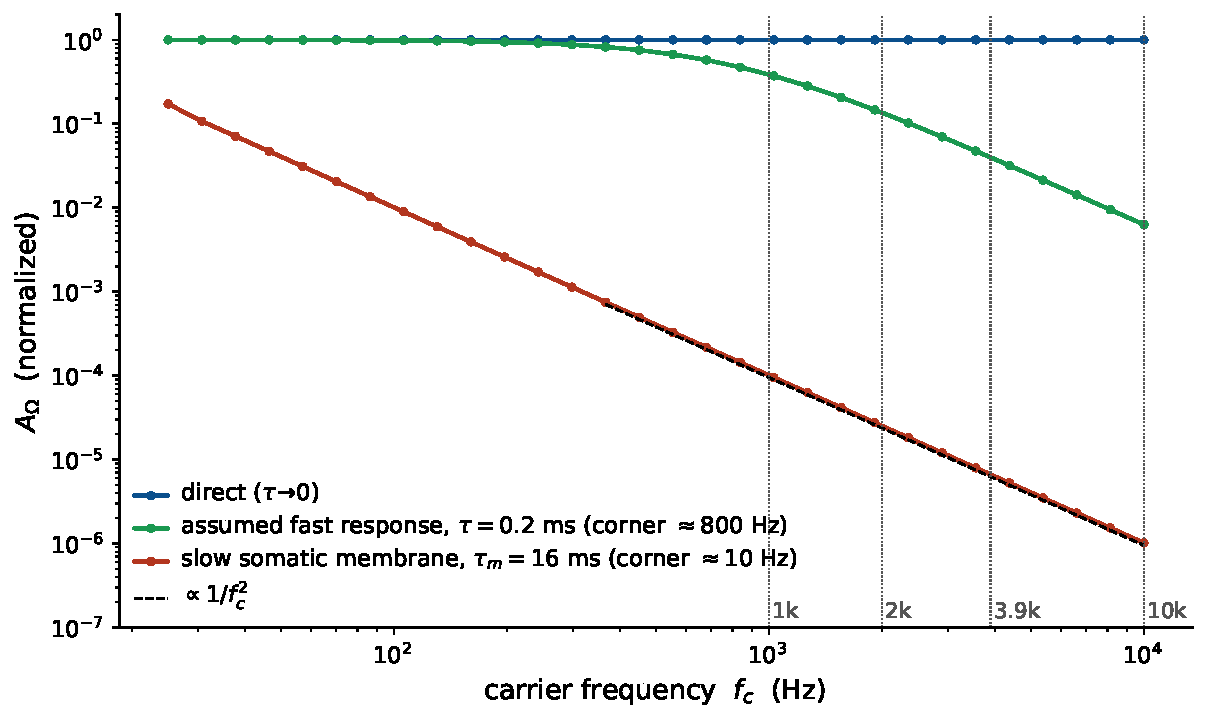
\includegraphics[width=0.74\textwidth]{fig_khz.pdf}
\caption{\textbf{Carrier attenuation depends on the assumed access time (Jansen--Rit, open loop).} Open-loop
demodulated response (normalized to the $\tau\!\to\!0$ value) vs.\ carrier
frequency up to $10$~kHz. With direct coupling ($\tau\!\to\!0$) the response is
flat---carrier-independent. A slow somatic membrane ($\tau_m\!\approx\!16$~ms)
rolls off as $1/f_c^2$ (dashed guide); the assumed fast response
($\tau=0.2$~ms) retains about $0.14$ of the direct response at $2$~kHz and $0.04$
at $3.9$~kHz. These are sensitivity cases, not measurements of anatomical
compartments.}
\label{fig:khz}
\end{figure}

\setcounter{figure}{5}
\begin{figure}[t!]
\centering
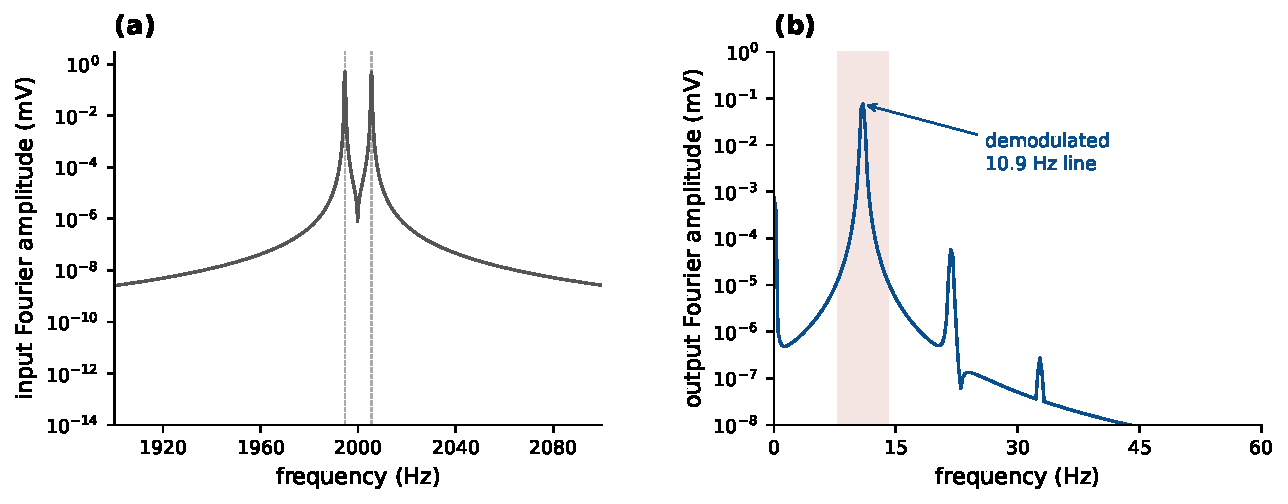
\includegraphics[width=0.95\textwidth]{fig_khz_twotone.pdf}
\caption{\textbf{Two-tone TI at a kHz carrier (Jansen--Rit, assumed fast access).}
Two equal tones at $f_1=1994.543$ and $f_2=2005.457$~Hz, beating at
$10.914$~Hz, pass through the assumed low-pass ($\tau=0.2$~ms) into the recurrent column.
\emph{(a)} The input amplitude spectrum has lines only at $f_1$ and $f_2$; in the
$8$--$14$~Hz band its maximum is $2.2\times10^{-13}$~mV.
\emph{(b)} The output carries a demodulated line at the beat, $10.9$~Hz.}
\label{fig:khz_twotone}
\end{figure}

\setcounter{figure}{8}
\begin{figure}[t!]
\centering
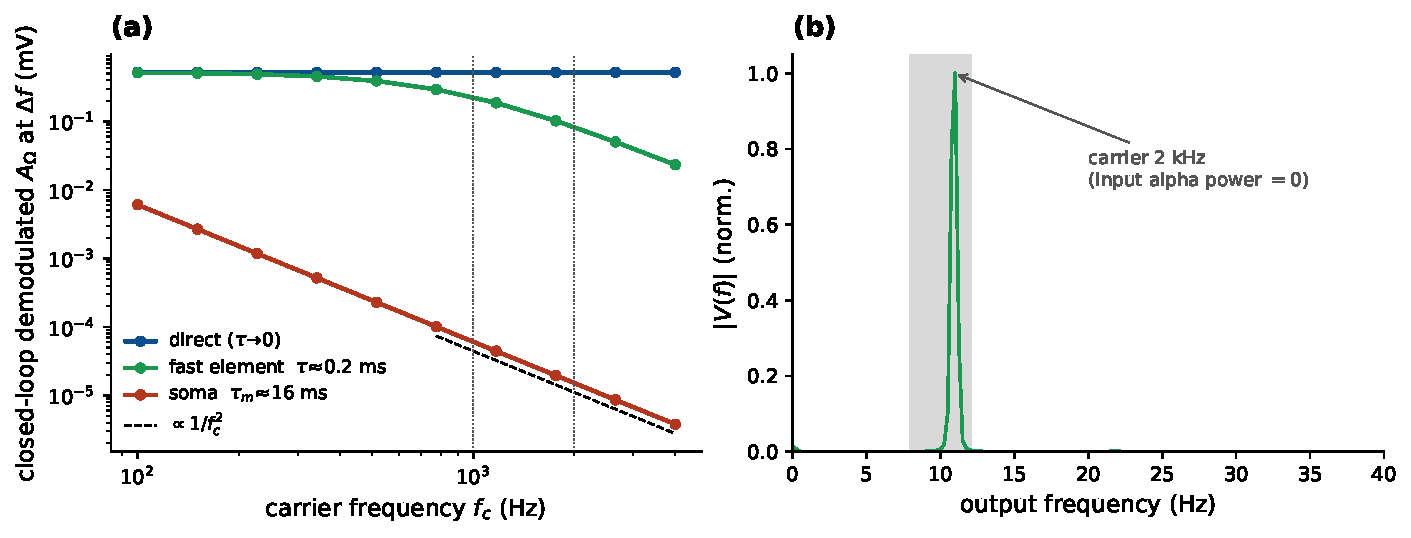
\includegraphics[width=\textwidth]{fig_khz_direct.pdf}
\caption{\textbf{Demodulation at a kHz carrier (Jansen--Rit, closed loop).}
The applied field passes through an explicit membrane filter before the sigmoid.
\emph{(a)} Closed-loop demodulated $A_\Omega$ at $\Delta f=f_0$ vs.\ carrier $f_c$ for
three access models: direct ($\tau\!\to\!0$, carrier-independent), fast
($\tau=0.2$~ms), and somatic ($\tau_m=16$~ms; $1/f_c^2$ roll-off).
The fast time is assumed rather than assigned to a measured compartment.
\emph{(b)} Output spectrum for a
$2$~kHz carrier delivered through the fast element: an alpha line at $f_0$,
synthesized by the column although the input carries no alpha power.}
\label{fig:khz_direct}
\end{figure}


\section{Detection and harmonic signatures}\label{supp:detection}
These calculations support the carrier-scaling and harmonic tests in
\S\ref{sec:transduction} and the dynamic detector in \S\ref{sec:dynamic}.
\subsection{Fixed-voltage mixing and carrier exponents}\label{supp:dynamic-details}
Time and frequency use the membrane-time units defined in article
Appendix~\ref{app:mpr-coefficients}; $r^*,d,\nu$ have the same definitions.
Membrane access is already included in this calculation. The linear voltage response
is $H_v(\omega)=(i\omega+d)/[(i\omega+d)^2+\nu^2]$. Dividing by its squared magnitude
gives the mixing coefficient at fixed voltage excursion,
\begin{equation}
\kappa_V(Q,\omega)=\frac{\kappa_{\rm DC}(Q,\omega)}{|H_v(\omega)|^2}
=\frac{F'(Q)}{2}\;\frac{\omega^2+3d^2-\nu^2}{\omega^2+d^2}.
\label{eq:kfixed}
\end{equation}
This coefficient tends to $F'/2$ at high frequency. The $1/\omega^2$ suppression
at fixed current comes from $|H_v|^2$, the membrane filtering already represented
by \ifsupp main-text\fi\ Eq.~\eqref{eq:doors}; it is not an additional detector filter. A static curve
placed after the same membrane has the same leading carrier roll-off, although
its mixing coefficient and sign can differ. The steady-state curvature is
$F''=4r^*(3d^2-\nu^2)/(d^2+\nu^2)^3$, so the inflection occurs at $\nu^2=3d^2$.

For nearby fast tones, the quadratic terms in \ifsupp main-text\fi\ Eq.~\eqref{eq:mpr} contribute at
different orders: $v^2$ at $\omega^{-2}$, $r v$ at $\omega^{-3}$, and $r^2$ at
$\omega^{-4}$. Table~\ref{tab:exponents} compares the carrier and beat routes to
the firing rate for a static curve and a dynamic population with the same membrane access.

\begin{table}[h]
\centering\small
\begin{tabular}{lcc}
\toprule
stage & static curve, same membrane & dynamic population \\
\midrule
point-membrane current $\to$ voltage & $\omega^{-1}$ & $\omega^{-1}$ \\
voltage $\to$ rate, carrier & $1$ & $\omega^{-1}$ \\
current $\to$ rate, carrier & $\omega^{-1}$ & $\omega^{-2}$ \\
two tones $\to$ beat in the rate & $(\omega_1\omega_2)^{-1}$ & $(\omega_1\omega_2)^{-1}\times$ const. \\
\bottomrule
\end{tabular}
\caption{Fast-carrier scaling with matched point-membrane access, at fixed beat frequency
and a nonzero leading mixing coefficient. The dynamic population integrates the
carrier once more between voltage and rate; the beat is formed before that step.
Prefactors depend on the operating point and beat-frequency susceptibility.}
\label{tab:exponents}
\end{table}

The first row gives the shared membrane factor $1/\omega$. The second converts
voltage to rate: a static curve adds its slope, whereas the dynamic rate equation
integrates the carrier once more. Combining these stages gives the third-row
carrier responses, $\omega^{-1}$ and $\omega^{-2}$, respectively.

The beat in the last row is formed before that additional rate integration:
static curvature and dynamic $v^2$ each mix the attenuated voltage, retaining
$(\omega_1\omega_2)^{-1}$. Equal exponents do not imply equal amplitudes; mixing
and the susceptibility at fixed $\Omega$ determine the prefactors. For the
uncoupled carrier-averaged response, $\kappa_V$ in Eq.~\eqref{eq:kfixed} tends to
$F'/2$, but is not the full finite-$\Omega$ network prefactor. Thus the dynamic
rate attenuates the carrier twice while forming the beat between those stages.

\ifjne
\subsection{Harmonic ladder and mixed detectors}\label{supp:harmonics}
\DIFaddbegin \DIFadd{Full- and half-wave rectifiers yield $2\mathcal A/\pi$ and
$\mathcal A/\pi$, respectively; a diode-and-capacitor detector follows the
peak. Channel rectification, threshold crossing, and release events are
possible biological implementations.
}

\DIFaddend Envelope following and square-law detection are distinguishable at a single site. At a matched target,
$\mathcal A(t)=2\varepsilon|\cos(\Omega t/2)|$, whose Fourier series
$|\cos\theta|=\tfrac2\pi+\tfrac4\pi\sum_{n\ge1}\tfrac{(-1)^{n+1}}{4n^2-1}\cos(2n\theta)$ gives a
harmonic ladder whose nonnegative Fourier amplitudes $A_{n\Omega}$ obey $A_{2\Omega}/A_\Omega=1/5$, $A_{3\Omega}/A_\Omega=3/35$ and
$A_{4\Omega}/A_\Omega=1/21$. The square-law output $\half \mathcal A^2=\varepsilon^2(1+\cos\Omega
t)$ contains only DC and $\Omega$. For the mixed family $T(\mathcal A)=c_1\mathcal A+c_2\mathcal A^2$, with
$c_1\ne0$ and a nonzero fundamental, the
pre-network ratio is
\begin{equation}
\mathcal H_{\rm det}\equiv\left|\frac{Y_{2\Omega}}{Y_\Omega}\right|
=\frac{1/5}{\left|1+\tfrac{3\pi}{4}\,c_2\varepsilon/c_1\right|},
\label{eq:rdet}
\end{equation}
so measuring $\mathcal H_{\rm det}$ constrains $c_2\varepsilon/c_1$ within this family.\footnote{The inverse has two branches unless the sign of the fundamental
relative to the linear term is known; for $c_2/c_1\ge0$ it is unique.}

\fi
\subsection{AM-surrogate and genuine two-tone comparisons}\label{supp:waveform-checks}
These checks support the waveform choices in \S\ref{sec:waveforms}. Agreement
at the leading beat does not imply equal steady sources or driven operating states.

\begin{table}[htbp]\centering\small
\caption{Waveform comparisons at the stated operating points. JR response ratios
use the same voltage readout; timing ratios use the same pyramidal firing rate.}
\label{tab:waveform-checks}
\begin{tabular}{@{}p{4.3cm}p{4.5cm}p{6cm}@{}}
\toprule
Comparison & Conditions & Result\\
\midrule
JR open-loop beat & $v^*=8$ mV & Two-tone/AM: $1.0000$ at $0.02$ mV; $0.988$ at $1$ mV.\\
JR modulation/mean shift & Pinned sweep: far from Hopf, $\gamma=1$ s$^{-1}$, nearest point & Two tones: $14.5$, $58$, $44$; AM: $19$, $66$, $45$. AM has $3/4$ of the two-tone direct steady source.\\
JR TI/tACS output & Far from Hopf, $\gamma=1.07$ and $0.12$ s$^{-1}$ & AM: $0.14$, $0.24$, $0.47$; two tones: $0.14$, $0.24$, $0.46$. Difference at most $2.2\%$ across the grid.\\
JR matched-source output & Three couplings, settings in \S\ref{app:jr-sweep-settings} & TI/tACS: $0.99$, $0.94$, $0.92$ for AM; $0.99$, $0.93$, $0.90$ for two tones.\\
PING beat & Well below Hopf; $\bar\eta=0.9$ & Matched AM and two-tone responses agree within $0.07\%$ and $4\%$, respectively.\\
\bottomrule
\end{tabular}
\end{table}

\subsection{The cubic Hopf normal form lacks a quadratic mixer}\label{app:sl}
The Stuart--Landau equation \cite{pikovsky2001}
\begin{equation}
\dot z=(\alpha+i\omega_0)z-|z|^2z+\mathcal F(t),\qquad
\gamma=-\alpha>0,
\label{eq:sl}
\end{equation}
uses seconds for time and a normalized complex mode $z$, with the cubic
coefficient set to $1$~s$^{-1}$. Its linear growth rate is $\alpha=-\gamma$;
$\gamma$ has units s$^{-1}$. The mode has damping $\gamma$ and natural angular frequency
$\omega_0$, driven by the applied input $\mathcal F$ (normalized mode units per second). For a weak input
$\mathcal F=\varepsilon_{\rm SL} \psi_{\rm SL}(t)$ with dimensionless waveform $\psi_{\rm SL}$ on the stable side, the perturbative response has
the form $z=\varepsilon_{\rm SL} z_1+\varepsilon_{\rm SL}^3z_3+\cdots$. There is no second-order
source: the first-order response contains only the applied frequencies, and the
cubic first contributes at order $\varepsilon_{\rm SL}^3$. Thus the normal form has a
resonant linear susceptibility but lacks the quadratic difference-frequency
generation of \ifsupp main-text\fi\ Eq.~\eqref{eq:demod}. This statement concerns the weak-input
expansion; it is not an exclusion of every higher-order intermodulation or
strong-drive response.

In the numerical control ($\alpha=-0.5$~s$^{-1}$, $f_0=10$~Hz, $f_c=100$~Hz,
$\varepsilon_{\rm SL}=0.5$~s$^{-1}$), a square-law detector gives a beat-frequency lock-in amplitude
of $2.5\times10^{-1}$, while $\mathrm{Re}\,z$ gives approximately
$2\times10^{-8}$, at the numerical floor. Driving the same mode directly in band
recovers the forced $1/\gamma$ growth. The control separates resonant amplification
from the nonlinear source required to drive it at the beat.

\section{Spatial maps}\label{supp:spatial}
These definitions and checks support the geometric maps in \S\ref{sec:fem-results}
and the interpretation of mean-square polarization in \S\ref{sec:dc}.
\ifjne
\subsection{Envelope-mean subharmonicity}\label{supp:envelope-proof}
The envelope mean \DIFdelbegin \DIFdel{has the same restriction}\DIFdelend \DIFaddbegin \DIFadd{is
}\[
\DIFadd{\overline{\mathcal A}(\mathbf x)=\frac{1}{2\pi}\int_0^{2\pi}
\sqrt{\varepsilon_1(\mathbf x)^2+\varepsilon_2(\mathbf x)^2
+2\varepsilon_1(\mathbf x)\varepsilon_2(\mathbf x)\cos\vartheta}\,\mathrm d\vartheta,
}\]
\DIFadd{where $\vartheta$ is beat phase.
}

\DIFadd{For fixed scalar coupling in homogeneous, isotropic, source-free tissue,
the envelope mean is subharmonic}\DIFaddend . At each beat phase $\vartheta$,
$\mathcal A$ is the Euclidean norm of
$(\varepsilon_1+\varepsilon_2\cos\vartheta,\,\varepsilon_2\sin\vartheta)$,
a vector of harmonic functions. A norm is convex, so this envelope is subharmonic;
averaging over $\vartheta$ preserves that property. Thus both idealized mean maps
lack a strict interior maximum under these conditions (Fig.~\ref{fig:spatial_maps}b).

\subsection{Isotropic orientation averages}\label{supp:orientation}
For isotropically distributed unit orientations
$\mathbf n$ with orientation-independent access and curvature,
$\langle(\mathbf n\cdot\mathbf E_j)^2\rangle=|\mathbf E_j|^2/3$
and $\langle(\mathbf n\cdot\mathbf E_1)(\mathbf n\cdot\mathbf E_2)\rangle
=\mathbf E_1\cdot\mathbf E_2/3$: orthogonal fields cancel the averaged beat,
but retain the DC intensity.

\fi
\ifjne
\subsection{Head-model procedure}\label{supp:fem-protocol}
To compare the spatial predictions on the same anatomy, we compute all maps
in one open-access subject,
IXI002 of the IXI dataset\footnote{\url{https://brain-development.org/ixi-dataset/}}
(T1-weighted MRI; female, 35 years). The T1 image was segmented into six tissues
(scalp, skull, cerebrospinal fluid, gray matter, white matter and eyes) and meshed with
SimNIBS~3.2.3 \texttt{headreco} \cite{nielsen2018}, with its CAT12 option
\cite{gaser2024}. Tissue conductivities were 0.33 (scalp), 0.008 (skull), 1.79
(cerebrospinal fluid), 0.40 (gray matter), 0.15 (white matter) and 0.33~S/m (eyes)
\cite{salvador2025}. These are low-frequency values; no dispersion correction was
applied at the kHz carriers. The volume conductor is linear and quasi-static, so the
carrier frequencies do not enter the maps.

The electrodes follow the published hippocampal montage of Violante et al.\
\cite{violante2023}, placed by its recipe on the subject's registered 10--10
positions. Pair~1 (anterior) joins e1, 25~mm from T9 toward FT9, to e2, 10~mm from AF8
toward Fp2. Pair~2 (posterior) joins e3, 25~mm from T9 toward TP9, to e4, 10~mm from P8
toward PO8. Each electrode is a 20-mm disc of 3~mm of gel (4.0~S/m) under 2~mm of metal
(10~S/m), meshed into the head model with SimNIBS~3.2.3; the resulting mesh has
$3.64\times10^6$ linear tetrahedra. As a montage sensitivity, the 10--10 rendering of
this montage, FT7--F8 (anterior) and TP7--P8 (posterior), which Yatsuda et al.\
\cite{yatsuda2024} used as their starting montage, was meshed and solved in the same
way. Each montage has its own mesh, carrying only its own four electrodes.

Each pair was solved once at 1~A. The potential $\phi_j$ (V) satisfies
$\nabla\!\cdot\!(\sigma_{\rm cond}\nabla\phi_j)=0$, where
$\sigma_{\rm cond}$ is tissue conductivity (S/m). Current enters and leaves through each
electrode's metal contact as a Neumann condition, distributed in proportion to nodal
area; the rest of the scalp carries no normal current, and one pinned node fixes the
gauge. The linear finite-element system was assembled and solved with Neuroelectrics'
temporal-interference library, by conjugate gradients with algebraic-multigrid
preconditioning, to a relative residual of $10^{-8}$. The field
$-\nabla\phi_j$ was recovered at gray- and white-matter
nodes by superconvergent patch recovery \cite{zienkiewicz1992}, separately within each
compartment (446{,}877 node--compartment pairs). Dividing these fields by the solve
current gives the field-per-current vectors $\mathbf F_j$, expressed in
(V/m)/mA to match $I_j^{\rm pair}$. Every current condition is a scaling of these two fields.
With peak pair currents $I_1^{\rm pair}$ (anterior) and
$I_2^{\rm pair}$ (posterior) summing to 4~mA, the ratio 1:1 is $2+2$~mA and 1:3 is
1~mA anterior plus 3~mA posterior, the two conditions of Violante et al. The ratio sweep
sets the posterior share $I_2^{\rm pair}/(I_1^{\rm pair}+I_2^{\rm pair})$ from 0.1 to
0.9 in steps of 0.025.

The field-to-polarization conversion follows \S\ref{sec:envelope}:
$\varepsilon_j(\mathbf x)=I_j^{\rm pair}\mathcal P_j(\mathbf x)$, with
$\mathcal P_j=\lambda_0\,\mathbf F_j\!\cdot\!\mathbf n$, one uniform
static coupling $\lambda_0=0.5$~mV per V/m \cite{radman2009}, and
$\lambda_f\approx\lambda_0$. A uniform coupling multiplies the envelope map by
$\lambda_0$ and the two second-order maps by $\lambda_0^2$. Target-to-reference ratios,
normalized maps and focus positions do not depend on it. Hippocampal couplings of
$0.12$--$0.18$~mV per V/m \cite{bikson2004,deans2007} would scale the absolute values
by $0.24$--$0.36$ and $0.06$--$0.13$, respectively.

The detector compartment fixes the projection direction. A laminar direction for a pyramidal
axon initial segment, a local axon direction for a node, or an orientation
distribution for terminals defines a different access model. Isotropic averaging
is one possible distribution, not an anatomical consequence of choosing terminals.
Maximizing a geometric map over orientation gives an upper bound for that map
at each location; it does not identify the detector's orientation.

The projection direction $\mathbf n(\mathbf x)=\mathbf n^*(\mathbf x)$ is the envelope-maximizing direction at
the reference ratio 1:1: the closed-form maximizer, over unit vectors, of
$2\min(|\mathbf F_1\!\cdot\!\mathbf n|,|\mathbf F_2\!\cdot\!\mathbf n|)$
\cite{grossman2017}. It is chosen once at each node and then held fixed for 1:1, 1:3
and every ratio of the sweep, and all three maps use it. Along it, the 1:1 envelope map
equals its maximum over orientation. At any other ratio it is the envelope seen by an
element with that fixed orientation, which can be below that ratio's own maximum. As an
orientation sensitivity, every statistic was repeated along a second fixed field, the
radial direction from the brain centroid. The isotropic comparison averages the signed
mixing term over uniformly distributed orientations before its magnitude is taken:
$\langle\varepsilon_1\varepsilon_2\rangle_{\mathbf n}
=\lambda_0^2I_1^{\rm pair}I_2^{\rm pair}\,\mathbf F_1\!\cdot\!\mathbf F_2/3$, so the
isotropic beat excursion is
$\tfrac23\lambda_0^2I_1^{\rm pair}I_2^{\rm pair}|\mathbf F_1\!\cdot\!\mathbf F_2|$.
Elements whose beats have opposite phase cancel in this average.

The target is the left hippocampus of a FreeSurfer~6.0.0 \texttt{recon-all}
segmentation of the same T1 image (\texttt{aseg} label 17, 3903~mm$^3$)
\cite{fischl2002}. The region of interest (ROI) is the 1{,}568 gray- and white-matter
nodes inside it. The reference is the 273{,}544 gray-matter nodes outside the
ROI, including other deep gray matter. It is a gray-matter reference, not a cortex-only contrast.
The mesh and the segmentation share one image frame; tissue-volume, centroid and
white-matter checks confirmed their alignment. As a label sensitivity, the
Neuromorphometrics atlas hippocampus, warped into the subject with SimNIBS~3.2.3
\texttt{mni2subject} and the subject's nonlinear MNI transform (1{,}345 nodes; Dice 0.72
with the FreeSurfer label), replaced the ROI. As a tissue sensitivity, the ROI was
restricted to its gray-matter nodes (1{,}174 with the FreeSurfer label, 1{,}013 with
the atlas label).

The target-to-reference ratio is the ROI 95th percentile divided by the reference
95th percentile; its mean-based companion divides the ROI mean by the same
reference percentile. All percentiles and centroids weight nodes equally.
The quadratic excursion and $\mathcal I$ are second order in the field, whereas
the envelope excursion is first order. To separate this difference in degree
from the spatial weighting, each second-order statistic is also given
degree-matched, computed on the square root of the map. This is a geometric
comparison; the raw maps remain the respective detector predictions before gain.
The focus is the centroid of the top 10\% of ROI nodes,
ranked by the map's own value, with 5, 25 and 50\% as a sensitivity. Ranking makes the
focus exactly invariant to a uniform positive factor. Its displacement from 1:1 is
measured along the hippocampal long axis, the first principal axis of the ROI nodes,
with anterior positive. Field projections still use $\mathbf n^*$, independently
of this reporting axis. The 1:1 to 1:3 displacement was computed for every combination
of montage, label, ROI tissue definition and focus fraction (32 per map), each montage
along its own 1:1 direction.

No signed DC-source or mean-response map is computed. For a spatially uniform detector
coefficient, $Y_{\rm DC}=\tfrac12\Sig''(v^*)\mathcal I$ (\S\ref{sec:dc}) is
$\mathcal I$ rescaled, with the sign of $\Sig''(v^*)$. A nonuniform coefficient would
require an operating-point map, which a head model does not provide, and a mean
response would additionally require a circuit model. In particular,
$\Sig''(v^*)$ is curvature at the population model's operating point, not a
measurement of the transfer at the axon initial segment. Assigning that
coefficient to an anatomical detector requires a calibrated access and
input--output model.

\subsection{Sensitivity of focus displacement}\label{supp:fem-sensitivities}
The spatial ordering in the article persists across montage, labeling, tissue,
and focus-fraction choices. Table~\ref{tab:fem-sensitivities} gives the ranges;
orientation changes absolute contrast more than the atlas label in this subject.
For the reference projection and label, the top-5--50\% focus moves
$2.2$--$4.0$~mm anteriorly for the envelope and $2.4$--$8.2$~mm posteriorly
for mean-square polarization.

\DIFaddbegin \DIFadd{The sweep shows two kinds of steering (Fig.~\ref{fig:fem}e,f). The envelope ratio peaks
near balance ($1.24$ at a posterior share of $0.525$) and falls to $0.89$--$0.94$ at
the extremes. Its focus moves only while the two carriers are comparable inside the
hippocampus. At a posterior share of $0.6$ or more, the anterior pair is the weaker
carrier at more than 96\% of hippocampal nodes; at $0.4$ or less, the posterior pair is. The
envelope map then equals twice the weaker pair's polarization over most of the ROI,
and its measured focus changes little with further imbalance. The focus of $\mathcal I$ moves
continuously instead, from $1.5$~mm anterior at a posterior share of $0.1$ to $6.3$~mm
posterior at $0.9$, while its ratio stays between $0.79$ and $0.94$ ($0.89$--$0.97$
degree-matched). The quadratic excursion keeps one ratio and one focus across the
whole sweep.
}

\DIFaddend \begin{table}[htbp]\centering\small
\caption{Focus displacement from 1:1 to 1:3. Envelope shifts are anterior;
mean-square shifts are posterior. The quadratic beat shift is zero in every case.
Contrasts quoted in the last column are raw 1:1 envelope/quadratic contrasts.}
\label{tab:fem-sensitivities}
\begin{tabular}{@{}lrrl@{}}
\toprule
Sensitivity & Envelope (mm) & Mean square (mm) & Contrasts\\
\midrule
Atlas label & $2.0$--$3.8$ & $3.2$--$5.9$ & $1.17$ / $1.04$\\
Radial direction & $1.9$--$2.8$ & $2.0$--$3.7$ & $1.62$ / $1.97$\\
All 32 combinations & $0.7$--$8.1$ & $0.5$--$10.6$ & \\
\bottomrule
\end{tabular}
\end{table}

\subsection{\DIFdelbegin \DIFdel{Mean-square change }\DIFdelend \DIFaddbegin \DIFadd{Envelope and mean-square changes }\DIFaddend under current-ratio steering}\label{supp:steering-algebra}
The mean-square polarization
changes by $\mathcal I_{1:3}/\mathcal I_{1:1}
=(\mathcal P_1^2+9\mathcal P_2^2)/[4(\mathcal P_1^2+\mathcal P_2^2)]$,
exceeding one only where $|\mathcal P_2|>\sqrt{3/5}|\mathcal P_1|
\approx0.775|\mathcal P_1|$. Its hippocampal mean rises by 24\% and its focus
moves 4.5~mm posteriorly. Equal summed currents therefore do not match local
RMS polarization.

\DIFaddbegin \DIFadd{Local envelope excursion increases under 1:3 where
$|\mathcal P_1|>2|\mathcal P_2|$, reaching $1.5\times$ where
$|\mathcal P_1|\geq3|\mathcal P_2|$. A selective or thresholded envelope
response therefore remains possible despite the lower ROI mean excursion.
}

\DIFaddend \fi
\setcounter{figure}{12}
\begin{figure}[t!]
\centering
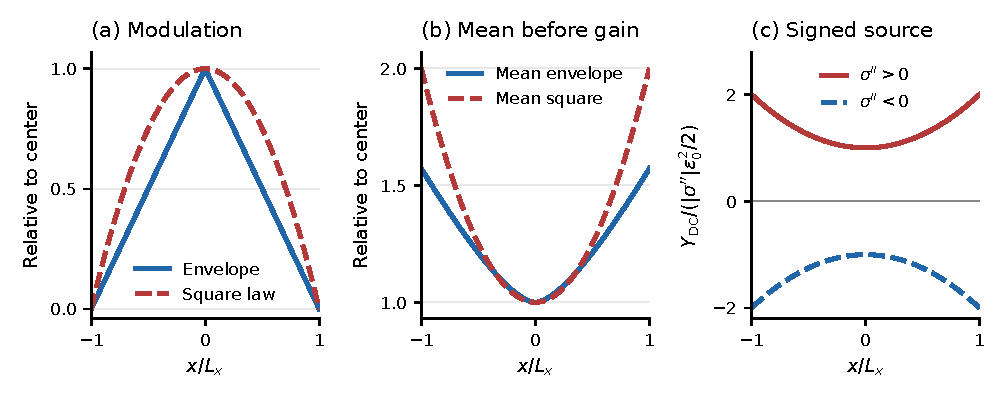
\includegraphics[width=\textwidth]{fig_spatial_maps.pdf}
\caption{\textbf{Envelope and quadratic spatial maps.} Illustrative line profile:
$\varepsilon_1(x)=\varepsilon_0(1+x/L_x)$ and
$\varepsilon_2(x)=\varepsilon_0(1-x/L_x)$ on $-L_x\le x\le L_x$, with polarization scale
$\varepsilon_0>0$ (mV) and length $L_x>0$ (m). In (a,b), each geometric curve is
divided by its own positive value at $x=0$.
\emph{(a)} Modulation is $1-|x/L_x|$ for envelope following and $1-(x/L_x)^2$ for quadratic
detection: both peak centrally, but the quadratic profile is broader here.
\emph{(b)} The mean envelope and mean-square polarization $\mathcal I$ both
increase toward the edges; neither includes a signed detector gain.
\emph{(c)} The static JR rate source $Y_{\rm DC}=\Sig''\mathcal I/2$ for uniform
positive curvature (solid red) or negative curvature of the same magnitude
(dashed blue). Both use the same positive scale $|\Sig''|\varepsilon_0^2/2$,
giving $\pm[1+(x/L_x)^2]$; the gray line marks zero. These are assumed detector
states before recurrent feedback, not inferred physiological responses.
This is a line profile, not a head model or a demonstration of three-dimensional focusing.}
\label{fig:spatial_maps}
\end{figure}


\section{Recurrent amplification and numerical checks}\label{supp:amplification}
These protocols support the coupling, timing, and field-induced gamma results in
\S\ref{sec:jcurve}--\S\ref{sec:qif}.
\subsection{JR coupling-sweep settings}\label{app:jr-sweep-settings}
The coupling sweeps of Figs.~\ref{fig:jcurve} and~\ref{fig:timing}, and the transcranial
alternating-current stimulation (tACS) control of Fig.~\ref{fig:tacs}, use the single JR
column with the field-free operating point $v^*$ pinned: for
each global connectivity $C$ we solve the field-free fixed-point relation analytically
for the external drive $p(C)$ that holds $v^*$ (hence $\Sig''(v^*)$) fixed, vary $C$
toward the alpha Hopf, and read $\gamma,\omega_0$ from the $6\times6$ Jacobian. The field
is the AM surrogate of \ifsupp main-text\fi\ Eq.~\eqref{eq:amsur} for Fig.~\ref{fig:jcurve}, genuine two
tones for the timing comparison (Fig.~\ref{fig:timing}), or a direct in-band sinusoid $s(t)=\varepsilon\cos\Omega t$
($\varepsilon=0.1$~mV) for the tACS control (Fig.~\ref{fig:tacs}), each read out by the
lock-in of $v$ at $\Delta f$, except in the timing comparison, which reads the
modulation and mean of the same pyramidal rate $r_P=\Sig(v+s)$.
That comparison uses $18$~s settling and a $20$~s window for each waveform.
The Figure~\ref{fig:jcurve}--Figure~\ref{fig:tacs} response-ratio comparison uses
$v^*=8.30$~mV, TI surrogate amplitude $0.3$~mV with $m=1$ and $f_c=100$~Hz,
and tACS amplitude $0.1$~mV, driven at each field-free modal frequency.
The original TI amplitudes are interpolated logarithmically in $C$ onto the tACS
grid. For the waveform comparison, both the surrogate and two-tone TI are rerun
on that grid with $12$~s settling and a $6$~s window.
Pinning fixes the background curvature; it does not cancel the stimulation-induced
mean shift.
Additional controls at $C=110$, $133.9091$, and $136.3$ use a tACS amplitude of
$0.0143039$~mV, matched to the leading TI beat source. They record mean voltage,
mean rate, and lock-in with $12$~s settling and a $6$~s window, repeated with
$60$~s settling and a $20$~s window; the latter settings also test genuine two tones.


\ifjne
\subsection{PING coupling-sweep settings}\label{supp:ping-runs}
We compute the linear reference's
second-order source from the PING quadratic terms at the central carrier,
$300$~Hz, and apply the full linearized network response over $15$--$90$~Hz
in $0.025$~Hz steps. Using the distinct AM sidebands changes the peak gain by
less than $0.1\%$ across this sweep.

The simulated coupling sweep uses the AM surrogate, $A_f=8$, with $5$~s
settling and a $4$~s window. We search around each linear resonance, extending
the frequency grid until each sampled maximum is bracketed, and compare
amplitudes $A_f=2,4,8$ at nine couplings. Local parabolic interpolation changes
the sampled peaks by less than $1.3\%$. The figure scales the linear reference
to the median measured gain over $14.5<J<16$; the amplitude check instead
normalizes peak response divided by $A_f^2$ and linear gain to its value at
$A_f=2$, $J=15.53$. These normalizations compare gain variation with the detector coefficient
allowed to vary along this unpinned sweep\DIFaddbegin \DIFadd{.
}


\fi

\ifjne
\subsection{\DIFadd{Mode competition and finite-amplitude gain in PING}}\label{supp:ping-coupling-results}
\DIFadd{In NMM2 PING, $J$ is the mean inter-neuron QIF synaptic weight.
Sweeping $J$ at fixed background drive toward the gamma Hopf reveals two
competing modes (Fig.~\ref{fig:nmm2_jcurve}). A second mode near $55$~Hz carries
the linear-response peak over $14.6\lesssim J\lesssim16.2$; the critical mode
carries it at lower couplings and again near the Hopf, where its frequency is
about $50$~Hz. In that near-Hopf interval,
$0.0014\lesssim\gamma\lesssim0.0081$~ms$^{-1}$, the linear gain scales as
$1/\gamma$ with a fitted exponent of $1.02$ over a $5.8$-fold damping range.
The full-sweep exponent is $0.71$, so a single-mode law does not describe the
whole curve. Coupling-dependent sensitivity \cite{clusella2023} therefore
includes changes in which mode carries the peak.
}

\DIFadd{At $A_f=8$, the simulated response exceeds the normalized linear reference by
up to $48\%$ in the amplitude check, then saturates. At a quarter of that
amplitude ($A_f=2$, one sixteenth of the power), the departures stay within
$11\%$ at the nine tested couplings. The driven endpoint remains attracting under both waveforms
(\S\ref{app:ping-stability}).
The alpha JR and gamma NMM2 circuits share the $1/\gamma$ gain scaling of their critical mode despite their different
mixers, with amplification adjustable through coupling.
}

\subsection{\DIFadd{TI/tACS ratios and finite-amplitude saturation}}\label{supp:tacs-saturation}
\DIFadd{Table~\ref{tab:waveform-checks} gives the AM and genuine two-tone response
ratios for the three coupling controls specified in
\S\ref{app:jr-sweep-settings}. The predicted linear ratio is $0.143$ for
the unequal amplitudes in Figs.~\ref{fig:jcurve} and~\ref{fig:tacs}; the
common transfer cancels at a fixed state. The stronger direct response
saturates earlier near the Hopf: multiplying its input by $6.99$ increases
its output by only $6.97$, $3.95$, and $1.96$ at those three couplings.
Stimulation-induced mean shifts, which field-free pinning does not cancel,
account for the departure from the linear ratio. These are not equal-RMS
comparisons; matching conventions are given in \S\ref{sec:direct-comparison}.
}

\subsection{\DIFadd{QIF integration and matched-carrier protocol}}\label{supp:qif-protocol}
\DIFadd{The finite network uses the PING model and observables defined in
\S\ref{sec:qif-methods}. The following settings support the weak-drive and
field-induced gamma comparisons.
}

\DIFadd{Euler integration uses $0.0025$~ms steps and $800$~ms settling, exceeding
four field-free relaxation times at $\bar\eta=0.85$ ($176$~ms).
Measurements cover whole beat cycles to avoid phase-coverage bias:
$44$ at $55$~Hz and $34$ at $42$~Hz ($800$ and $810$~ms).
}

\DIFadd{We also run both conditions at $A_f=10$ per tone with the same measurement
settings. For $\bar\eta=0.85$, separate checks double the population size,
double the measurement window, or halve the integration step; further runs raise
$V_{\rm peak}$ to $200$ and $400$ at both time steps. An equal-RMS
mean-field control replaces the two tones by one $300$~Hz carrier with peak
amplitude $\sqrt{2}A_f$, using the same duration: both inputs have mean-square
amplitude $A_f^2$ over these windows. The carrier comparison starts from the
field-free equilibrium and uses $800$~ms settling and $800$~ms measurement,
with a $3200$~ms window to check spectral leakage at the larger amplitude.
}

\DIFadd{A longer window reduces the single carrier's apparent $55$~Hz
depth from $0.011$ to $9.2\times10^{-5}$, while TI's stays at $0.30$--$0.31$;
the former is spectral leakage}\DIFaddend .

\fi

\subsection{Stability of the driven PING endpoint}\label{app:ping-stability}
We check the stability of the driven $J$-curve endpoint by integrating the full
variational matrix along its trajectory. At carrier $300$~Hz and beat $50.5$~Hz,
the AM input repeats every $2$~s. After $8$~s of settling, we compute the
perturbation multipliers over that period and repeat over the next period.
Moduli below one indicate decay of perturbations to the periodic response.
Two-tone controls at $J=16.5663$ and $16.5901$, both with a $50.5$~Hz beat,
use $5$~s settling, direct perturbation decay, and an $8$~s finite-time
Lyapunov estimate.

Although a DC-only averaged calculation predicts an unstable endpoint, the full
periodically forced solution remains attracting: its largest perturbation
multiplier is $0.034$ over the $2$~s forcing period. Increasing settling from
$0.6$ to $3$~s changes the endpoint lock-in by $0.8\%$. With genuine two tones,
the $50.5$~Hz endpoint control also attracts nearby trajectories: perturbations
decay at $-0.0014$~ms$^{-1}$, and the $8$~s Lyapunov estimate is
$-0.00079$~ms$^{-1}$. These controls test a nonlinear driven response, not linear
gain about the DC-shifted equilibrium.

\subsection{Finite-network numerical checks}\label{app:qif-checks}
At $A_f=10$ and $\bar\eta=0.85$, the finite-network beat depth is $0.093$
for the published cutoff, versus the mean-field value $0.128$. Raising the spike cutoff from $V_{\rm peak}=100$ to
$200$ and $400$ gives depths $0.127$ and $0.139$, while the mean-rate increase
stays at $2.8$--$2.9\%$. At the original cutoff, doubling the population gives
$0.083$ and halving the time step gives $0.093$. The response is therefore
sensitive to the finite spike cutoff. Halving the step at cutoffs $200$ and
$400$ gives depths $0.121$ and $0.141$, respectively: cutoff dependence persists,
and quantitative convergence remains unestablished at this population size.
At the plotted cutoff, the pooled spike-phase vector strength is $0.046$;
median per-neuron phase consistency remains negative in field-off and field-on
windows at all three cutoffs.
In the $A_f=35$ convergence checks, halving the time step changes the lock-in and the pooled vector
strength by under $1\%$; doubling the spike-detection threshold changes the lock-in by
about $1\%$ and the mean rate by $2\%$, but the pooled vector strength at
$\bar\eta=0.85$ by about $45\%$, so phase concentration, unlike rate modulation, is sensitive to
how spike times are defined.


\ifjne
\subsection{A cutoff-free theta-neuron check}\label{supp:theta-pilot}
The change of variables $V_j=\tan(\theta_j/2)$ converts the QIF equation to
\[
\tau_X\dot\theta_j=(1-\cos\theta_j)
 +(1+\cos\theta_j)(\eta_j+U_X(t)),
\]
where $U_X$ is the same recurrent and external input as in the voltage model.
An upward crossing of $\theta=\pi$ emits a spike; wrapping by $2\pi$ replaces
the finite voltage cutoff and reset. We linearly interpolate the crossing
time for phase statistics. Empirical spike counts still drive the original
second-order synapses. Excitability quantiles, initial voltage, coupling,
carrier, and readouts are unchanged.

The pilot used $\bar\eta=0.85$, $A_f=10$, $f_c=300$~Hz, a $55$~Hz beat,
and $800$~ms settling. Before running it, we set a stopping rule: rate depth
must change by less than $5\%$ under separate step halving, population
doubling, and window doubling before extending this solver to carrier controls.
Table~\ref{tab:theta-pilot} gives every tested setting. Step and window changes
satisfy that criterion; population doubling does not, so the pilot stops.
No finite-network equal-RMS control was run.

\begin{table}[htbp]
\centering\small
\begin{tabular}{@{}lrrrrr@{}}
\toprule
Condition & $N$ per population & Step (ms) & Window (ms) & Mean E rate (Hz) & Beat depth\\
\midrule
Field off & 8000 & 0.0025 & 800 & 50.4 & 0.006\\
Two tones & 8000 & 0.0025 & 800 & 51.8 & 0.156\\
Half step & 8000 & 0.00125 & 800 & 51.8 & 0.155\\
Double population & 16000 & 0.0025 & 800 & 51.8 & 0.137\\
Double window & 8000 & 0.0025 & 1600 & 51.8 & 0.151\\
Exact mean field & $\infty$ & 0.0025 & 800 & 52.1 & 0.128\\
\bottomrule
\end{tabular}
\caption{Cutoff-free weak-drive checks. Depth is the rate lock-in divided by
mean rate. Relative to the two-tone baseline it changes by $-0.4\%$,
$-11.9\%$, and $-3.0\%$ under step, population, and window changes.
Only the baseline settings have a matched field-off run.}
\label{tab:theta-pilot}
\end{table}

Removing the cutoff raises the baseline depth from $0.093$ to $0.156$.
The three cutoff results are compatible with an inverse-cutoff correction:
a fit of $d_\infty-c/V_{\rm peak}$ gives $d_\infty=0.156$, with residuals
of about $0.002$. This agreement supports a cutoff contribution but does not
establish joint numerical convergence. Doubling the population moves the
theta result toward the exact mean field, while also increasing the largest
sampled Euler step in phase from about $1.5$ to $3.2$ radians. A combined
population and time-step limit remains untested.

Pooled spike-phase vector strength rises from $0.002$ without stimulation
to $0.068$--$0.077$ in the driven runs. Median per-neuron phase consistency
remains negative, from $-0.015$ to $-0.005$, and supplies no evidence for
strong individual phase locking. The finite network therefore supports the
presence of population-rate modulation; its quantitative weak-input depth
and agreement with the mean field remain unresolved.

\fi
\subsection{Fast-carrier estimate at the illustrated amplitudes}\label{app:qif-estimate}
The $A_f=35$ runs are finite-amplitude illustrations: the fast-carrier estimate gives a voltage excursion
$A_f/(\tau_E\omega_c)\approx1.2$ per tone in the model's voltage units. Its
rectified excitatory-drive shift is about $1.5$, compared with $0.12$ at
$A_f=10$. At $\bar\eta=0.85$, the Hopf threshold for a drive shift applied
only to the excitatory population is $\delta\eta_E^*\approx0.286$. The larger
field is therefore expected to cross this threshold, whereas the smaller one
remains below it.

For two nearby carriers, the fast-carrier approximation gives a constant shift
of the excitatory drive, $\delta\eta_E\simeq A_f^2/(\omega_c\tau_E)^2$, from the
quadratic voltage term. We refine this estimate using the full PING linear carrier
responses and their second-order DC source, then solve for the carrier-averaged
equilibrium and its stability, including the source's dependence on that equilibrium.
This approximation isolates the mean shift; direct two-tone integrations retain
the beat forcing and provide a separate check.

\setcounter{figure}{2}
\begin{figure}[t!]
\centering
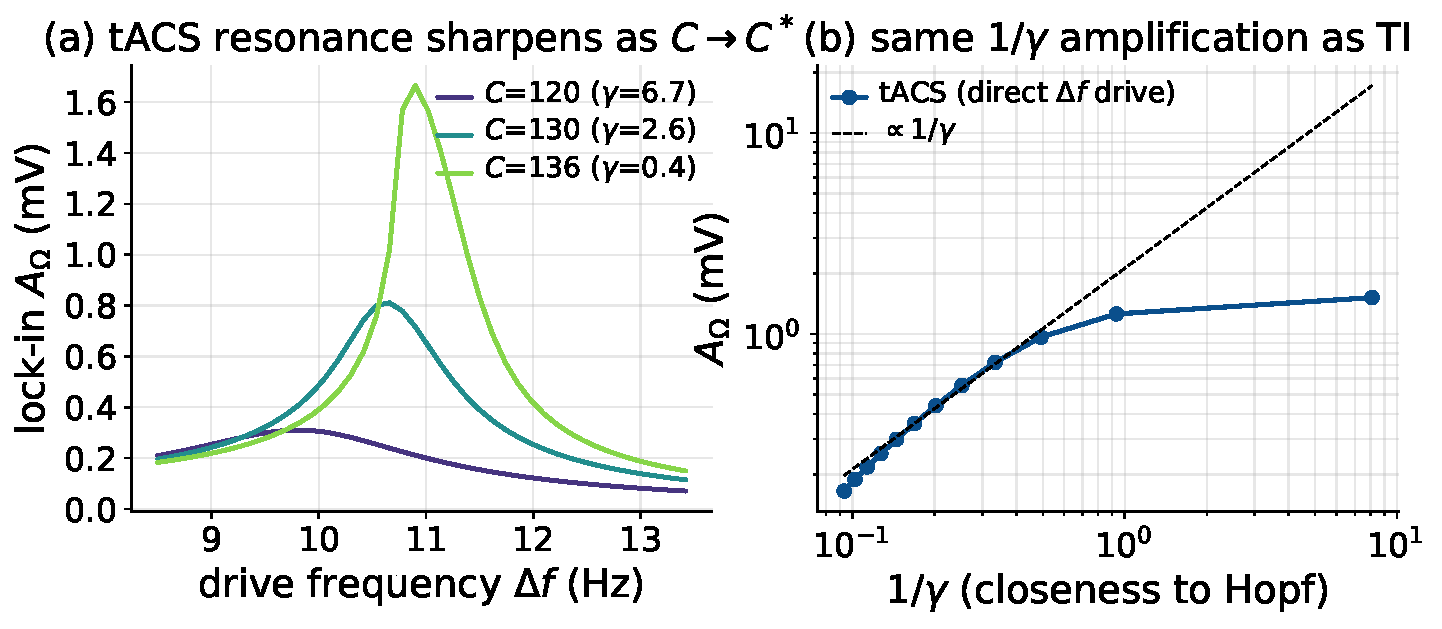
\includegraphics[width=0.92\textwidth]{fig_tacs_jcurve.pdf}
\caption{\textbf{tACS shares the network amplifier (Jansen--Rit).} A direct
low-frequency (tACS) drive at $\Delta f$ enters the column without a carrier, so it
needs no demodulation, but feeds the same near-Hopf resonator. With the field-free operating point
pinned, sweeping the coupling $C$ toward the alpha Hopf: \emph{(a)} the lock-in
resonance at $\Delta f$ sharpens and grows as $C\!\to\!C^*$; \emph{(b)} the response
grows as $1/\gamma$ (dashed) and saturates near criticality---the same network
amplification as the demodulated TI drive (Fig.~\ref{fig:jcurve}). The leading tACS
response is linear in the field; the TI beat is quadratic. Their response ratio
is independent of damping in linear response and changes at the finite amplitudes
nearest the Hopf (\S\ref{sec:jcurve}). Here $\gamma>0$ describes the field-free state.}
\label{fig:tacs}
\end{figure}

\setcounter{figure}{3}
\begin{figure}[t!]
\centering
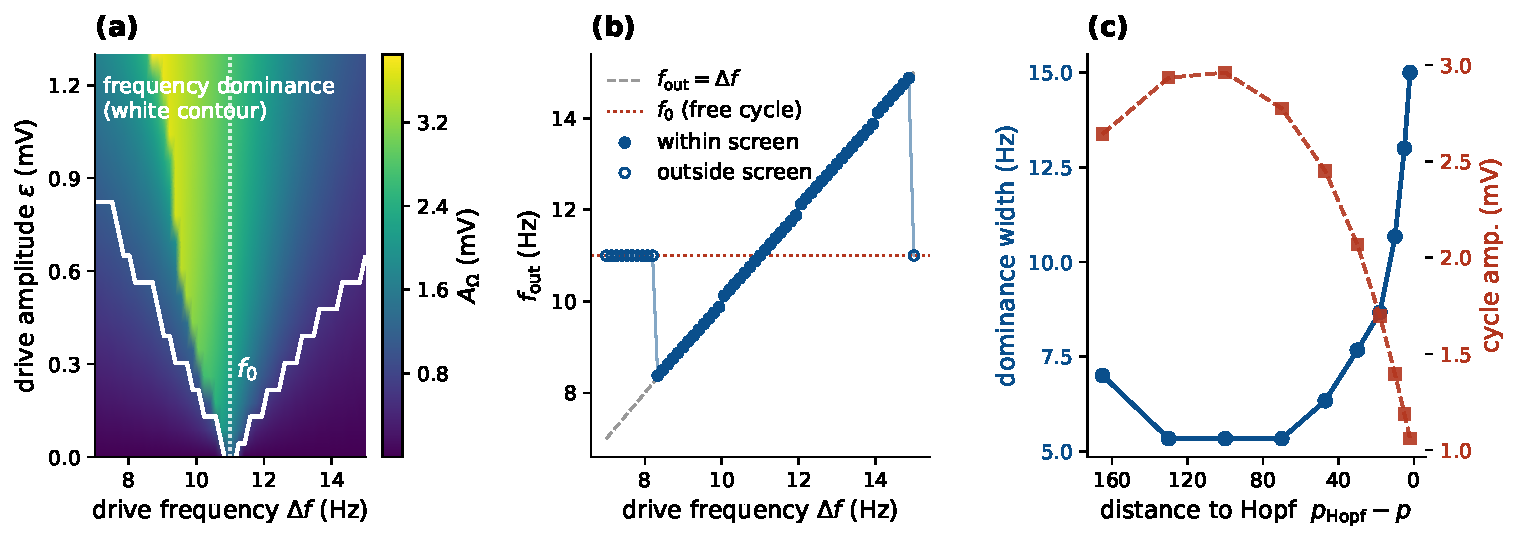
\includegraphics[width=\textwidth]{fig_entrainment.pdf}
\caption{\textbf{Frequency dominance in the driven autonomous Jansen--Rit column.}
The column is set in its autonomous alpha limit cycle ($p=250$, $f_0\!\approx\!11$~Hz) and
driven by a direct in-band sinusoid. \emph{(a)} The set
$|f_{\rm out}-\Delta f|<0.3$~Hz forms a wedge near $f_0$ that widens with drive.
It screens for phase capture but does not establish it. \emph{(b)} Inside this
region the dominant frequency follows $\Delta f$; outside, it remains near $f_0$.
\emph{(c)} Toward the Hopf at fixed drive the dominance width grows as the
autonomous cycle amplitude vanishes (blue, left axis; red dashed, right axis). Above the
Hopf this width describes frequency selection in a driven autonomous oscillator;
it is distinct from the linear susceptibility of the stable-focus side
(Fig.~\ref{fig:jcurve}). Both diagnostics increase toward criticality in these sweeps.}
\label{fig:entrain}
\end{figure}

\setcounter{figure}{7}
\begin{figure}[t!]
\centering
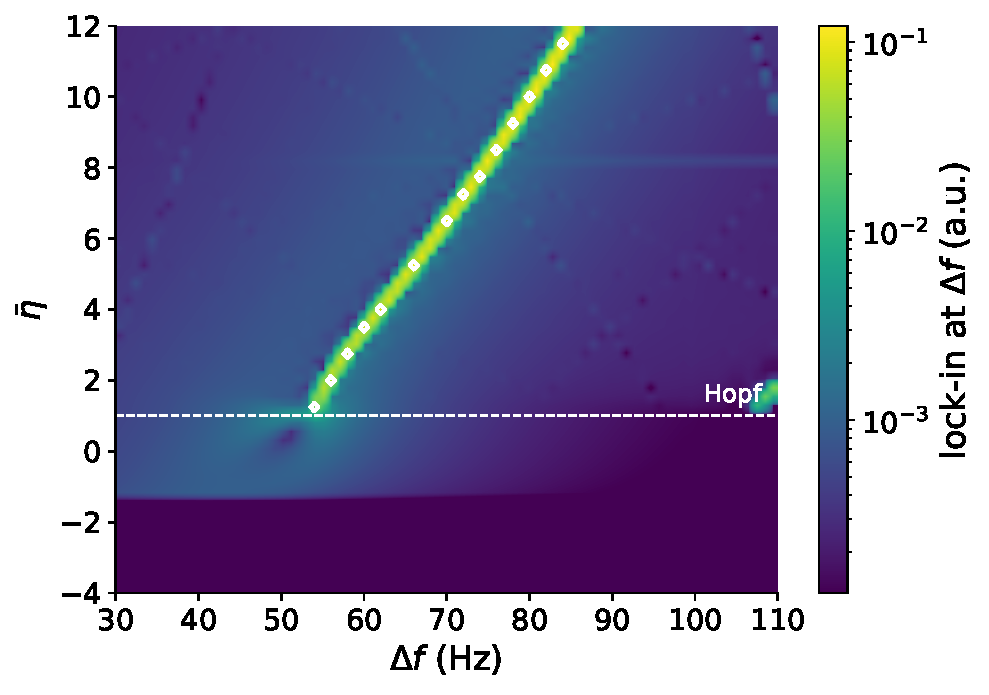
\includegraphics[width=0.72\textwidth]{fig_nmm2_map.pdf}
\caption{\textbf{NMM2 PING resonance map (exact mean field).} Demodulated response over
the ($\Delta f$, background drive $\bar\eta$) plane, log color scale. The ridge follows the
gamma natural frequency, with $f_0$ rising with $\bar\eta$ for these parameters. White markers
outline the frequency-dominance set (\S\ref{sec:vocab}), drawn only above the Hopf
(dashed line) where there is an autonomous rhythm to capture; below it the same color field
is a forced response. The markers do not establish phase capture. Lock-in amplitude
cannot separate driven and autonomous contributions, since both can place power at
$\Delta f$.}
\label{fig:nmm2_map}
\end{figure}

\setcounter{figure}{9}
\begin{figure}[t!]
\centering
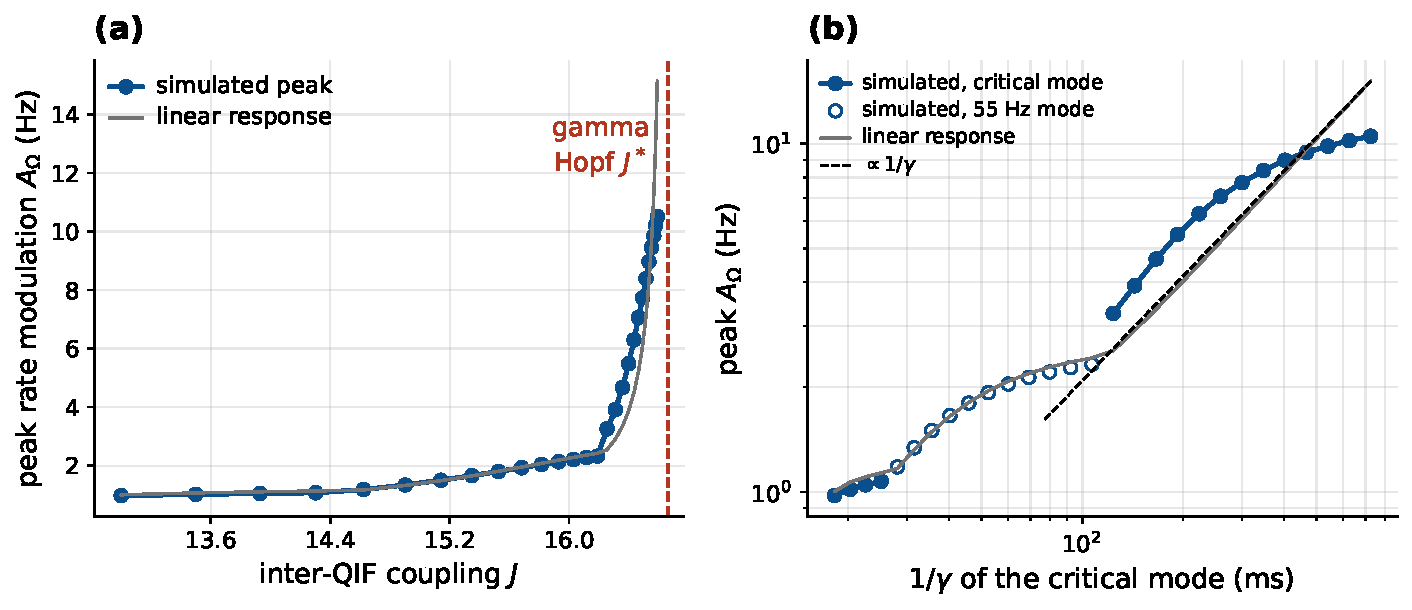
\includegraphics[width=0.92\textwidth]{fig_nmm2_jcurve.pdf}
\caption{\textbf{Coupling changes the dominant mode and its gain in NMM2.}
Unpinned sweep at $\bar\eta=0$, AM surrogate $A_f=8$.
\emph{(a)} Simulated rate peak (blue) and linear reference including the
second-order source (gray), normalized over $14.5<J<16$. Red dashed:
field-free Hopf. \emph{(b)} Gain against inverse damping of the critical
mode. Filled symbols: that mode carries the linear peak; open symbols:
the competing $55$~Hz mode carries it ($14.6\lesssim J\lesssim16.2$).
The dashed $1/\gamma$ guide is anchored at the last linear point.
The simulation exceeds then falls below the guide. The driven endpoint
remains attracting under both AM and genuine two-tone forcing.}
\label{fig:nmm2_jcurve}
\end{figure}

\setcounter{figure}{10}
\begin{figure}[t!]
\centering
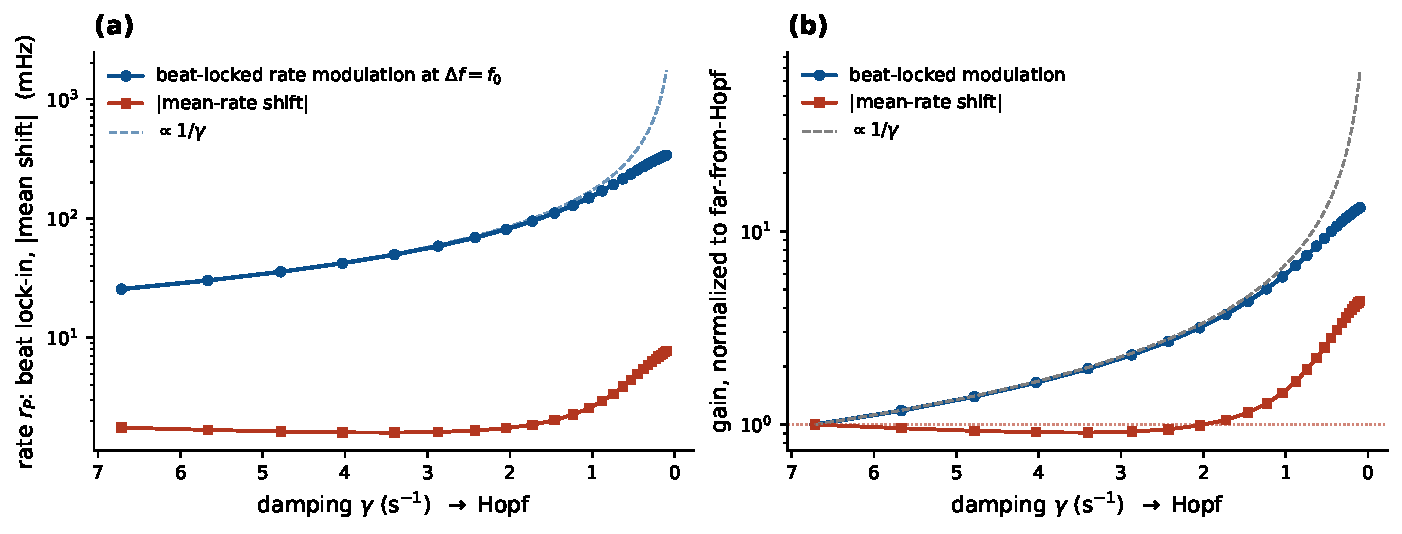
\includegraphics[width=\textwidth]{fig_timing_not_rate.pdf}
\caption{\textbf{Beat modulation grows more than the mean-rate shift.}
JR coupling sweep with fixed field-free curvature and genuine two-tone
input, $\Delta f=f_0$. Both observables use the pyramidal rate
$r_P=\Sig(v+s)$, in mHz.
\emph{(a)} Beat amplitude (blue) follows $1/\gamma$ (dashed) before
saturating; mean-shift magnitude (red) remains smaller.
\emph{(b)} Normalization to the far-from-Hopf values gives growth factors
$13.2$ and $4.4$. Their ratio rises from $14.5$ to $58$ near
$\gamma=1$~s$^{-1}$, then falls to $44$ as the amplified response rectifies.
The AM surrogate gives ratios $19$, $66$, and $45$.}
\label{fig:timing}
\end{figure}

\setcounter{figure}{11}
\begin{figure}[t!]
\centering
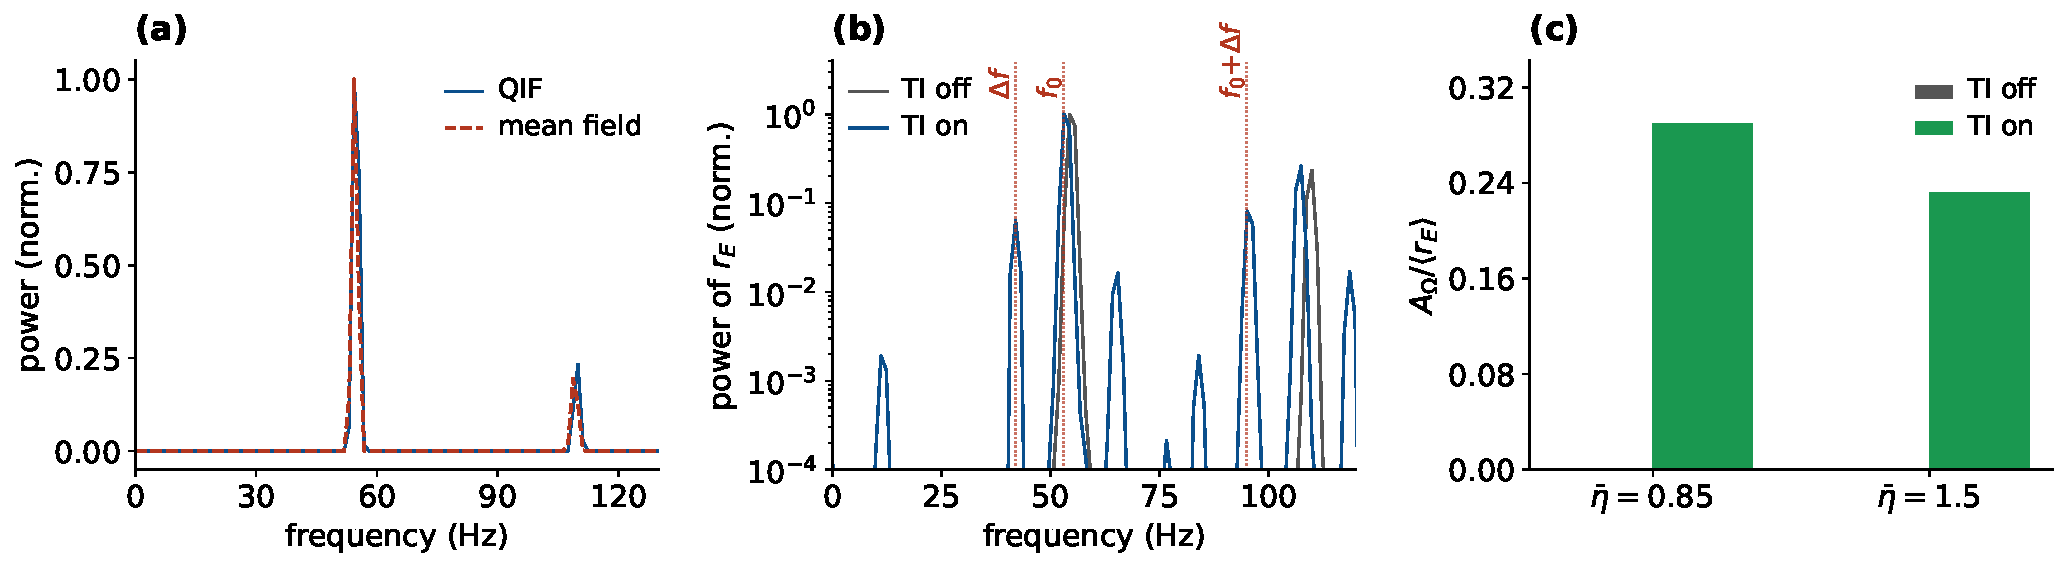
\includegraphics[width=\textwidth]{fig_qif_timing_twotone.pdf}
\caption{\textbf{Beat-locked modulation and mean-rate change in the QIF network.} \emph{(a)} Field-free power
spectrum of $r_E(t)$, normalized: the spiking network ($N=8000$) matches the exact NMM2
mean field in gamma frequency ($\sim$55~Hz); a normalized spectrum does not test the mean
rate. \emph{(b)} Intermodulation above the
Hopf (TI off vs.\ on, log power): the nonlinearity mixes the imposed $\Delta f=42$~Hz beat
with the persisting gamma near $53$--$54$~Hz, raising the direct $\Delta f$ line and the sum sideband
near $95$~Hz, both absent with TI off. These sidebands establish nonlinear mixing;
they do not uniquely identify gamma-amplitude gating. \emph{(c)} The $\Delta f$ modulation depth
$A_\Omega/\langle r_E\rangle$, off vs.\ on: below $0.003$ rising to $0.29$
($\bar\eta=0.85$) and $0.23$ ($\bar\eta=1.5$), while the mean rate rises by about
$8$--$11\%$. The labels identify field-free states; both field-on responses contain
gamma activity beyond the beat component. Spectra use the same post-settling windows
as the rate measurements and are normalized to each spectrum's maximum. Modulation depth is
reported rather than the off$\to$on lock-in ratio, whose denominator is the field-free
floor.}
\label{fig:qif_timing}
\end{figure}


\section{Efficiency of a memoryless transfer against a direct in-band drive}\label{app:bound}
For the logistic family of memoryless transfers, compare balanced TI tones of
polarization amplitude $\varepsilon$ each with a direct in-band drive of amplitude
$2\varepsilon$, matching peak polarization. Their leading drive amplitudes are
$|\Sig''|\varepsilon^2/2$ and $2\Sig'\varepsilon$, so
$\mathcal R_{\rm det}\simeq|\Sig''|\varepsilon/(4\Sig')$.
The weak-input formula concerns the logistic family. The step-mixture argument
below extends the exact carrier-averaged bound to bounded nondecreasing
memoryless transfers, with the same operating point, matched peak polarization,
and open-loop readout. It does not cover the dynamic detector of \S\ref{sec:dynamic}.

Writing $\zeta=\Sig/(2e_0)\in(0,1)$ gives
$\Sig'=2e_0\rho\zeta(1-\zeta)$ and
$\Sig''=2e_0\rho^2\zeta(1-\zeta)(1-2\zeta)$. Since
$|\mathrm{PEIX}|=1-4\zeta(1-\zeta)=(1-2\zeta)^2$, the leading ratio satisfies
\begin{equation}
\mathcal R_{\rm det}\simeq\frac{\rho\,\varepsilon}{4}\sqrt{|\mathrm{PEIX}|}
\;\le\;\frac{\rho\,\varepsilon}{4}.
\label{eq:etabound}
\end{equation}
It vanishes at the inflection, where the quadratic coefficient is zero, and
approaches its bound in the saturated tails. This maximizes a ratio rather than
an absolute response: both drives vanish in those tails. For the JR slope
$\rho=0.56$~mV$^{-1}$, the perturbative bound is $1.4\%$ at
$\varepsilon=0.1$~mV and $0.28\%$ at $\varepsilon=0.02$~mV.

Optimizing over the sigmoid slope gives a different limit from the weak-input bound.
The logistic transfer depends on voltage only through $\rho(v-v_0)$, so writing
\begin{equation}
u=\rho\,\varepsilon,\qquad \xi=\rho\,(v^*-v_0),
\label{eq:reduced}
\end{equation}
we have $\Sig(v^*+\varepsilon\psi(t))=2e_0\,L(\xi+u\,\psi(t))$ for any normalized waveform $\psi$,
with $L(\xi)=(1+e^{-\xi})^{-1}$. Every Fourier amplitude, and hence their ratio, is a function
of $(u,\xi)$ alone; the factor $2e_0$ cancels. Maximizing over $v^*$ and $\rho$ at fixed
$\varepsilon$ is therefore the same as maximizing over $(u,\xi)$, and the family supremum is
independent of field strength. Evaluating the exact cycle response rather than its
quadratic truncation and optimizing $\xi$ at each $u$, the ratio rises monotonically over the
range explored and converges to the hard-threshold limit
\begin{equation}
\sup_{\rho,\,v^*}\mathcal R_{\rm det}\approx0.3479 ,
\label{eq:etasup}
\end{equation}
approached as $\rho\to\infty$ at a threshold offset $\delta$ (the distance from the
operating point to the inflection) with $\delta/2\varepsilon=0.523$. There is no
finite optimal transfer width: narrower is always better, and reaching $95\%$ of the ceiling
requires $u\gtrsim6$, that is $1/\rho\lesssim\varepsilon/6$.

The limiting detector switches across its full range. At the optimum,
and at the illustrative fast-access polarization $\varepsilon\!\simeq\!0.1$~mV
of \S\ref{sec:discussion}, its open-loop beat drive
exceeds the physiological-slope sigmoid's by some three orders of magnitude for the same
$e_0$ and waveform, because the field excursion is about twice the threshold offset and the
transfer switches across its full range instead of responding linearly. The disparity grows
as the field weakens, the smooth sigmoid's response falling as $\varepsilon^2$ while a
threshold repositioned with the field keeps its excursion.

The required transfer width is small: at $\varepsilon=0.1$~mV the ceiling is approached only for
$1/\rho\lesssim17\;\mu$V; at $\varepsilon=0.02$~mV the corresponding width is
about $3\;\mu$V. Both follow from $1/\rho\lesssim\varepsilon/6$, with the
threshold offset held to the same order as the applied polarization. A population
sigmoid averages the spread of thresholds and noise; the JR voltage scale is
$1/\rho\approx1.8$~mV \cite{jansen1995}. A
microvolt width lies far below that and reads as an idealized microscopic threshold or
rectifier rather than as a neural-mass sigmoid; real thresholds are themselves noisy and
state-dependent, so it is not a measured single-cell property either. The
regime in which the family approaches its ceiling is thus one in which the ``population
sigmoid'' has ceased to describe a population.

The limit is a step detector, not an envelope follower. For a unit step at offset
$\delta$ the carrier-averaged transduction is $\pi^{-1}\arccos(\delta/\mathcal A)$ for $\mathcal A>\delta$
and zero below; with $\beta=\delta/2\varepsilon$ its tACS fundamental is
$(2/\pi)\sqrt{1-\beta^2}$ and its TI coefficient reduces by parts to
$\mathcal R_{\rm det}=2\beta\,[\mathsf K(k_{\rm ell}^2)-\mathsf E(k_{\rm ell}^2)]/(\pi\sqrt{1-\beta^2})$
with elliptic parameter $k_{\rm ell}^2=1-\beta^2$ and $\mathsf K,\mathsf E$
the complete elliptic integrals, giving $0.3479$ at $\beta=0.523$ by direct quadrature and
by the elliptic form alike (\texttt{threshold\_bound\_check.py}). At that optimum the
step's second-to-first harmonic magnitude ratio is $0.151$, not the $1/5$ of a linear
envelope follower. A bounded nondecreasing transfer is, up to a constant, a positive
mixture of shifted steps. Both signed Fourier coefficients are linear in the
transfer, and each step's direct-drive coefficient is nonnegative. The triangle
inequality therefore bounds the mixture's amplitude ratio by the largest step
ratio, whenever the denominator is nonzero. This extends the result beyond the
logistic family; the maximum itself is a numerical evaluation, not a certified bound.

\subsection{Experimental amplitude and phase-locking comparisons}\label{supp:vieira}
The protocols in Vieira et al.\ \cite{vieira2024} do not match local polarization at the detector.
The two-pair TI comparison gave a phase-locking effect ratio of $0.34$ against
tACS (95\% confidence interval $0.04$--$0.65$, 65 of 154 neurons), without
correcting for TI currents up to $\pm2.5$~mA per pair versus $\pm1$~mA for tACS.
A separate single-pair AM-tACS control compensated for frequency-dependent
shunting to match extracellular modulation depth. Of twenty cells, ten responded
to either modality and seven to both; in the latter group, median phase-locking
value (PLV) was $0.10$ for AM-tACS and $0.20$ for tACS, against $0.043$ at baseline.
The reported TI modulation depths were about $0.5$--$0.62$~V/m.


\section{Extension: the laminar column at low carriers}\label{app:lanmm}
The two-band laminar column (LaNMM) adds a resonant intermediary
between the field and the slow generator. These sweeps use $25$--$80$~Hz carriers
and polarizations up to $3$~mV on $P_2$, exceeding the sigmoid scale
$1/\rho\approx1.8$~mV. They describe nonlinear frequency selection below TI's
kHz range. The weak-field square law is tested separately in JR at
$0.05$--$0.2$~mV, one to two orders of magnitude below that scale
(Fig.~\ref{fig:opp}b).

\subsection{Model and measurements}\label{sec:lanmm-methods}
The laminar extension (LaNMM)
\cite{ruffini2025cfc,sanchezTodo2023} adds coupled alpha and gamma circuits: deep
pyramidal $P_1$, spiny-stellate (SS), and somatostatin (SST) populations, and a
superficial pyramidal $P_2$/PV circuit.
We simulate this laminar neural mass model (LaNMM). We integrate the full 28-variable column
\cite{ruffini2025cfc,sanchezTodo2023}, with the field entering as in the single
JR column, as a membrane polarization added inside the sigmoid argument of the target
population. Its output rate $\varphi_X$ (s$^{-1}$) is
\begin{equation}
\varphi_X(t)=\Sig\!\big(v_X(t)+s(t)\big),\qquad X\in\{P_1,P_2\},
\label{eq:lanmm_drive}
\end{equation}
with $s(t)$ the AM or two-tone field of \S\ref{sec:coupling} (amplitude $\varepsilon$ in
mV, beat $\Omega=2\pi\Delta f$, carrier $\omega_c=2\pi f_c$) and all three external drives
held flat at their baselines (Fig.~\ref{fig:lanmm_setup}). A perturbation of an external
input \emph{rate} would require clipping at zero
once its excursion exceeds the baseline, and a hard clip is a half-wave rectifier---a
diode detector placed upstream of the sigmoid, which would inject a line at $\Delta f$
into the drive before the population nonlinearity received it. A signed membrane
polarization carries no such constraint and none is applied. Because the LaNMM and JR
sigmoids share the voltage scale $1/\rho\approx1.8$~mV, $\varepsilon$ is directly
comparable between the two models.

Integration is a vectorized fixed-step RK4
($\Delta t=10^{-4}$~s) advancing the whole parameter grid simultaneously, as in the JR
sweeps. The maps report the
alpha-band ($8$--$12$~Hz) power of the $P_1$ and $P_2$ membrane potentials as the mean
squared magnitude of the Hann-windowed fast Fourier transform (FFT) over the band, in arbitrary units, over a
post-transient window. This measure includes autonomous and driven activity and
does not isolate a phase-coherent response to stimulation.

Two sweeps probe the column: an amplitude--beat sweep over
$(\varepsilon,\Delta f)$ at fixed carrier, and a carrier--beat sweep
over $(f_c,\Delta f)$ at fixed $\varepsilon$, built on the LaNMM module of
\cite{ruffini2025cfc}. The maps
(Figs.~\ref{fig:lanmm_p2},~\ref{fig:lanmm_p1}) show the \emph{signed} stimulation-induced
change, alpha power minus the unstimulated ($\varepsilon=0$) baseline, on a zero-centered
scale; over most of the $P_1$-driven grids the change is negative. For the
alpha resonance we instead drive the deep $P_1$ loop directly and sweep its input against
$\Delta f$, reading the lock-in (\ifsupp main-text\fi\ Eq.~\eqref{eq:lockin}) of $v_{P_1}$ at $\Delta f$.

The additional carrier comparison below uses the lock-in
of $v_{P_1}$, averaged at each carrier over 17 beats: $7$--$9$ and
$12.25$--$14$~Hz in $0.25$~Hz steps. These lie more than $1.5$~Hz from the
field-free alpha peak near $10.6$~Hz. We denote this arithmetic mean by $S(f_c)$.
The carrier grid is $25$--$80$~Hz in $1$~Hz steps, with equal tone amplitudes
$\varepsilon=1.5$~mV for $P_2$ drive and $0.5$~mV for $P_1$ drive. After $2$~s
of settling, we compare $3$ and $10$~s measurement windows. Field-free controls
give mean background amplitudes of $0.0048$ and $0.0012$~mV over the same beats.
This background includes a persistent component near $8$~Hz, so it is not solely
finite-window leakage. The statistic compares carrier profiles within each drive
condition; the unequal amplitudes do not support a direct sensitivity comparison
between targets.

\subsection{Frequency selection and carrier dependence}\label{sec:lanmm-results}
Driving either population with the two-tone field of Eq.~\eqref{eq:lanmm_drive}
and reading alpha-band power in the deep ($P_1$, alpha) and superficial ($P_2$,
gamma) pyramidal potentials recovers the beat resonance
(\S\ref{sec:lanmm-methods}, Fig.~\ref{fig:lanmm_setup}). Direct $P_1$ drive reproduces the JR
alpha-band resonance on both stable-focus and limit-cycle sides; that sweep
and its code are in the repository. The additional result is carrier selectivity
through the coupled gamma circuit.

Sweeping the field amplitude $\varepsilon$ and beat frequency $\Delta f$ at a fixed
carrier produces a region of enhanced alpha-band power: the response in $P_1$ is largest
when $\Delta f$ matches the deep alpha ($\sim$10~Hz) and grows with $\varepsilon$
(Figs.~\ref{fig:lanmm_p2}a,b and~\ref{fig:lanmm_p1}a,b). The dominant-frequency
contours identify where the output is close to the beat, without establishing
phase locking of the autonomous rhythm. Away from the enhancement region the drive
\emph{reduces} alpha-band power: with the field on $P_1$, $95\%$ of the amplitude--beat
grid and $97\%$ of the carrier--beat grid lie below the field-free baseline
(Fig.~\ref{fig:lanmm_p1}), the drive pulling the autonomous alpha out of the $8$--$12$~Hz
band or suppressing it; with the field on $P_2$ the fractions are $44\%$ and $31\%$
(Fig.~\ref{fig:lanmm_p2}).

The carrier dependence illustrates the two coupling limits of
\S\ref{sec:coupling}--\S\ref{sec:khz} within this model's $25$--$80$~Hz carrier
range. When the field is delivered to the superficial loop ($P_2$), alpha-band
power enhancement in $P_1$ is largest in the gamma carrier band with
$\Delta f$ near the $P_1$ alpha (Fig.~\ref{fig:lanmm_p2}c,d). At
$\Delta f=10$~Hz, the carrier maximum is $44$~Hz. This selectivity is consistent with a double
resonance: the fast loop acts as a tuned
radio-frequency (RF) front end whose dynamics affect the carrier dependence of
the deep response. With direct $P_1$ drive, a ridge near the column's own alpha
persists across the carrier range (Fig.~\ref{fig:lanmm_p1}c). That ridge contains
autonomous activity and is not a measurement of the demodulated component alone.

The lock-in also contains the autonomous rhythm when the beat is close to alpha;
its maximum over beats cannot isolate the driven response. We therefore compare
the off-alpha statistic $S(f_c)$ defined in \S\ref{sec:lanmm-methods}
(Table~\ref{tab:lanmm-carrier}).
With $P_2$ drive it peaks near $39$~Hz and falls to about $16$--$17\%$ of that
peak at a $25$~Hz carrier. With $P_1$ drive it peaks at $25$~Hz and spans about
$42$--$68\%$ of that peak over $30$--$80$~Hz. These are properties of the
specified amplitudes and beat average, not universal carrier-rejection factors.
Single-beat profiles have deeper minima, including a dip near a $45$~Hz carrier
under direct $P_1$ drive: the gamma circuit can affect the response in either
stimulation condition.

\begin{table}[t!]
\centering\small
\caption{\textbf{LaNMM carrier profiles measured away from alpha.}
$S(f_c)$ is the mean lock-in amplitude of $v_{P_1}$ over the 17 beats specified
in \S\ref{sec:lanmm-methods}. Percentages are normalized to each row's own carrier maximum;
the range and median use carriers from $30$ to $80$~Hz.}
\label{tab:lanmm-carrier}
\begin{tabular}{@{}llrrrr@{}}
\toprule
Drive & Window & Peak $S$ (mV) & Peak $f_c$ (Hz) & Range (\%) & Median (\%)\\
\midrule
$P_2$, $1.5$ mV & $3$ s  & $0.450$ & $39$ & $23$--$100$ & $42$\\
$P_2$, $1.5$ mV & $10$ s & $0.450$ & $39$ & $23$--$100$ & $42$\\
$P_1$, $0.5$ mV & $3$ s  & $0.092$ & $25$ & $42$--$68$  & $53$\\
$P_1$, $0.5$ mV & $10$ s & $0.091$ & $25$ & $42$--$67$  & $52$\\
\bottomrule
\end{tabular}
\end{table}

The carrier peaks and aggregate ranges persist with the longer window, although
individual normalized values change by up to $3.1$ percentage points for $P_2$
drive and $9.6$ for $P_1$ drive. The smallest $S$ exceeds its mean field-free
background by factors of about $16$ and $8$, respectively, with the $3$~s window,
and $62$ and $32$ with $10$~s. Some individual beat--carrier points remain near or below
background; the comparison concerns the mean over beats, not each grid point.
TI's kHz carriers lie outside this model's range. Within it, the carrier can
excite a network mode and affect the detected response, qualifying the inert-carrier
limit of \S\ref{sec:carrier} and linking it to frequency-tagging and
intermodulation paradigms \cite{gordon2019}.

\setcounter{figure}{0}
\begin{figure}[t!]
\centering
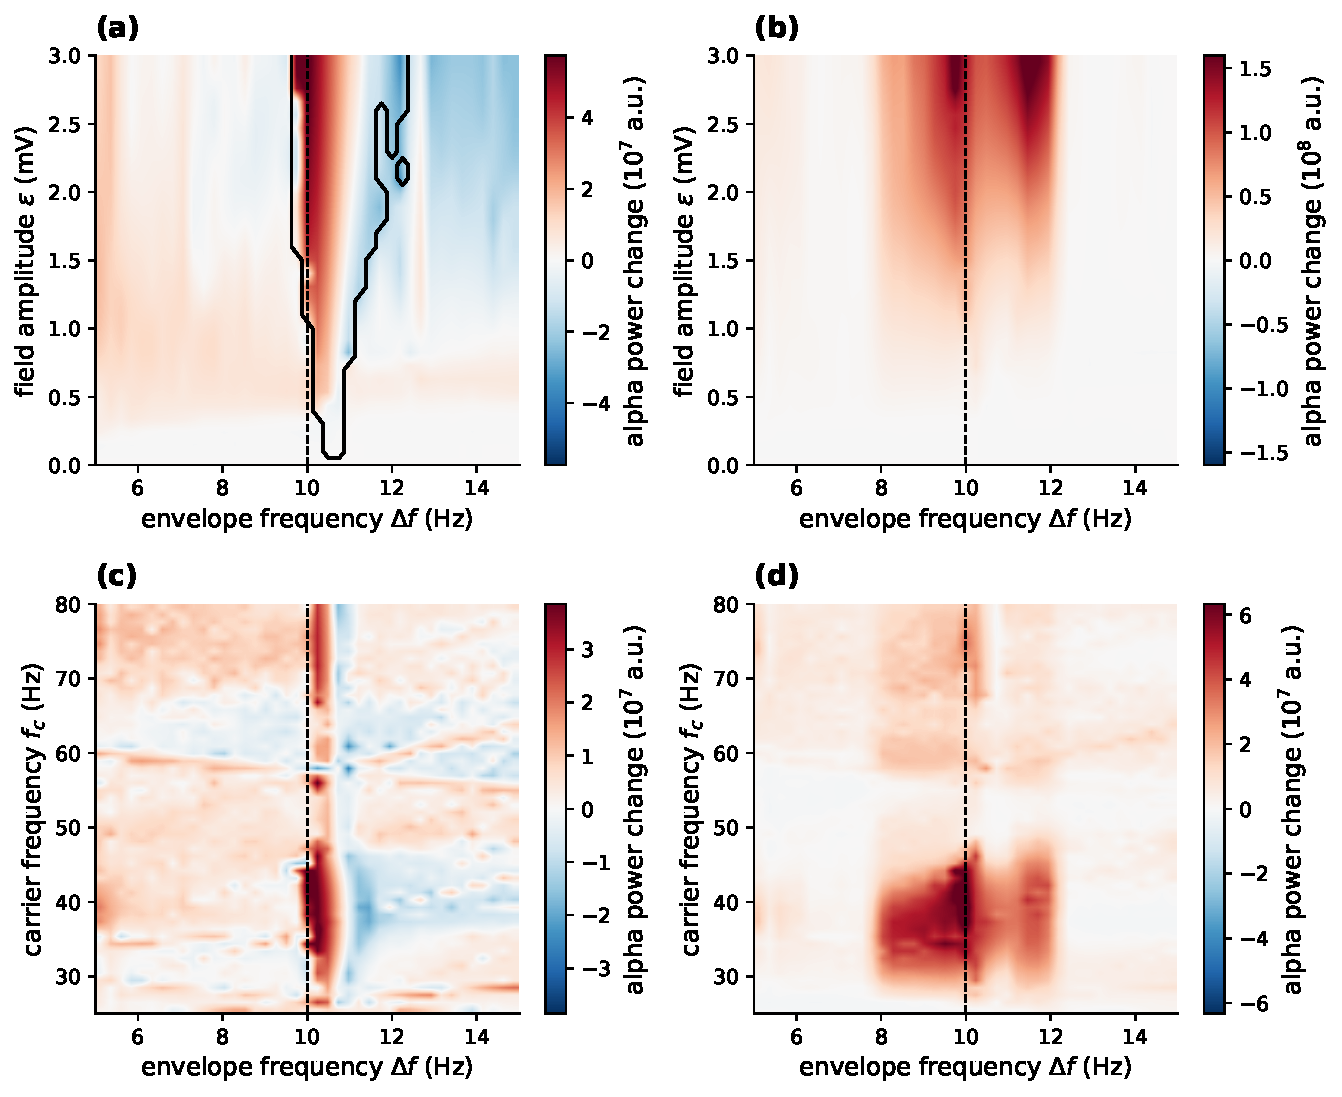
\includegraphics[width=0.86\textwidth]{fig_lanmm_field_p2_twotone.pdf}
\caption{\textbf{LaNMM frequency selection: two-tone TI field on the superficial $P_2$ (gamma)
loop.} The field enters the $P_2$ sigmoid argument as a membrane polarization $\varepsilon$
(mV) with all external drives flat. Color shows the signed change of alpha-band
($8$--$12$~Hz) power from the unstimulated $\varepsilon=0$ baseline, on a zero-centered
scale (arbitrary units). \emph{(a,b)} $P_1$ and $P_2$ enhancement vs.\
$\varepsilon$ and $\Delta f$ (carrier $40$~Hz), peaking at the $P_1$ alpha ($10.0$~Hz,
dashed). The black contour in \emph{(a)} is the frequency-dominance set
$|f_{\rm out}-\Delta f|<0.3$~Hz, drawn because band power
alone cannot separate a driven from an autonomous rhythm; it is a dominance screen, not a
phase-capture test. The $\varepsilon=0$ row is excluded, since with no drive the
autonomous $10.67$~Hz alpha already lies within the tolerance of two grid points (a
resolution floor of $0.5$~Hz); the set widens to $2.75$~Hz at $3$~mV. \emph{(c,d)} Enhancement vs.\ carrier and $\Delta f$ at
$\varepsilon=1.5$~mV: $P_1$ alpha-band enhancement is largest in the
gamma carrier band with $\Delta f$ near the $P_1$ alpha. At $\Delta f=10$~Hz,
the carrier maximum is $44$~Hz. The field-free
$P_2$ gamma peak is near $39.7$~Hz; the finite-drive maximum need not coincide with it.}
\label{fig:lanmm_p2}
\end{figure}



Within the $25$--$80$~Hz carrier range and at the finite polarizations used here,
the LaNMM shows alpha-band power changes concentrated near the intrinsic alpha,
amplitude-dependent widening of the frequency-dominance region, and enhanced
responses when superficial drive passes through the gamma circuit. The power
maps include autonomous and driven activity; they do not isolate TI efficacy.
The gamma-carrier preference, around $40$~Hz rather than kHz, remains a separate
prediction to test. Esmaeilpour et al.\ \cite{esmaeilpour2021} swept
$0.1$--$2$~kHz carriers at a fixed $5$~Hz beat against carbachol-induced gamma,
finding decreasing sensitivity with carrier frequency. Those carriers did not
sample the gamma band. Violante et al.\ \cite{violante2023} also used a fixed
$5$~Hz beat. Neither study tests this low-carrier resonance prediction.

\setcounter{figure}{1}
\begin{figure}[t!]
\centering
\setlength{\unitlength}{0.85\textwidth}%
\begin{picture}(1,0.8206)% original image aspect ratio
  \put(0,0){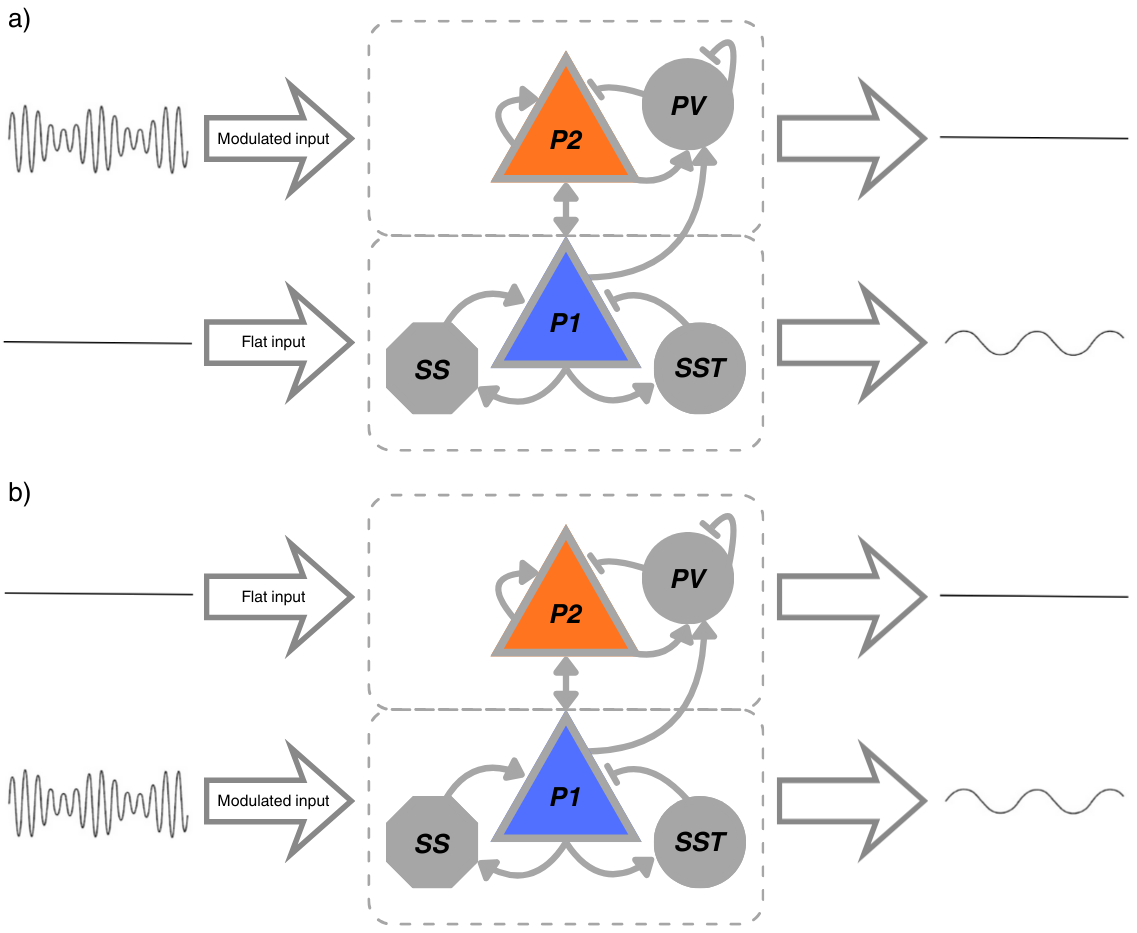
\includegraphics[width=\unitlength]{fig_lanmm_setup.png}}
  \put(0,0.788){\colorbox{white}{\makebox[0.045\unitlength][l]{\rule[-0.4ex]{0pt}{2.4ex}\textbf{(a)}}}}
  \put(0,0.371){\colorbox{white}{\makebox[0.045\unitlength][l]{\rule[-0.4ex]{0pt}{2.4ex}\textbf{(b)}}}}
\end{picture}
\caption{\textbf{Stimulation setup in a LaNMM column.} The column couples a
superficial PING subcircuit (pyramidal $P_2$ + PV; gamma) and a deep JR
subcircuit (pyramidal $P_1$ + SS + SST; alpha). \emph{(a)} the TI field drives
$P_2$ while $P_1$ receives a flat drive; \emph{(b)} the TI field drives $P_1$
while $P_2$ is flat. Through the sigmoid nonlinearities and $P_1$--$P_2$ coupling,
the generated beat-frequency component is transferred to the deep loop: $P_2$ carries the
modulated fast carrier, while $P_1$ exposes the recovered low-frequency component (right
traces).}
\label{fig:lanmm_setup}
\end{figure}

\setcounter{figure}{6}
\begin{figure}[t!]
\centering
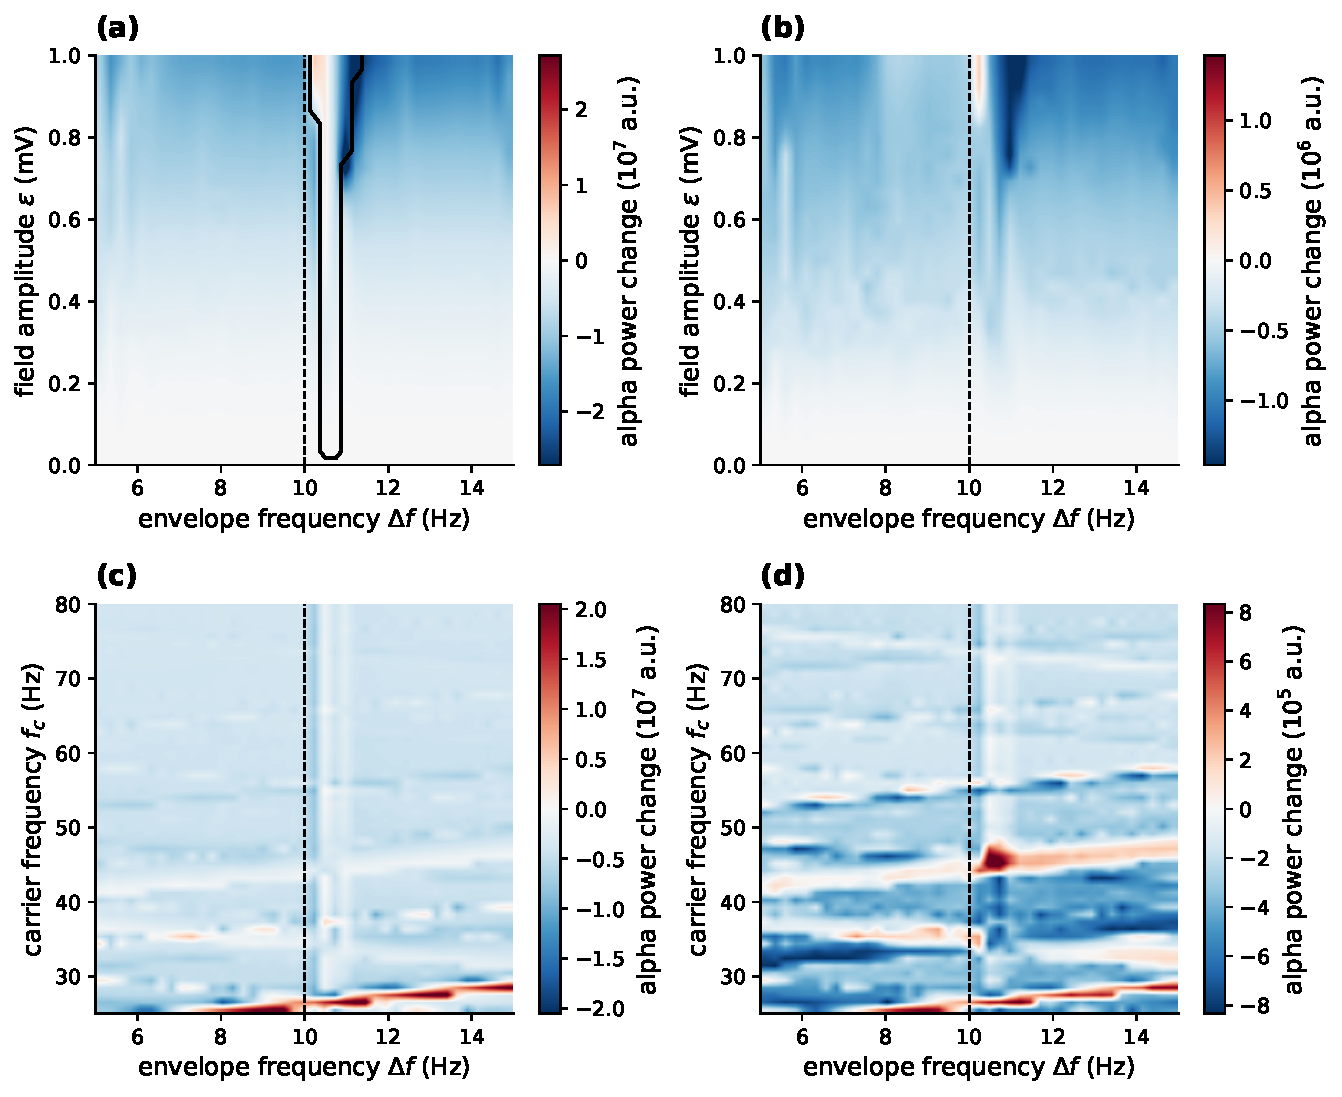
\includegraphics[width=0.86\textwidth]{fig_lanmm_field_p1_twotone.pdf}
\caption{\textbf{LaNMM frequency selection: two-tone TI field delivered directly to the deep
$P_1$ (alpha) loop.} As Fig.~\ref{fig:lanmm_p2} but with the field on $P_1$. The deep loop
shows frequency dominance at smaller fields, so the amplitude range is
$\varepsilon\le1$~mV here against $3$~mV there. These finite-amplitude maps extend
beyond the perturbative regime of the theory. Color: signed change of alpha-band power from the $\varepsilon=0$ baseline,
zero-centered; most of the grid is suppression. \emph{(a,b)} $P_1$ and $P_2$ enhancement vs.\ $\varepsilon$ and $\Delta f$; the
black contour in \emph{(a)} outlines the frequency-dominance set
$|f_{\rm out}-\Delta f|<0.3$~Hz (\S\ref{sec:vocab}), computed from the dominant
output frequency because band power alone cannot separate a driven from an autonomous
rhythm; the $\varepsilon=0$ row is excluded (resolution floor $0.5$~Hz). The set widens to
$1.25$~Hz at $\varepsilon=1$~mV.
\emph{(c,d)} Enhancement vs.\ carrier frequency and $\Delta f$ at $\varepsilon=0.5$~mV.
The ridge near alpha persists across the carrier band and includes the autonomous
rhythm. A separate lock-in comparison away from alpha, including its window and
background controls, is given in Table~\ref{tab:lanmm-carrier}; these panels show
band-power changes.}
\label{fig:lanmm_p1}
\end{figure}


\section{Experimental tests and numerical definitions}\label{sec:vocab}
\emph{Forced response.} Below the Hopf the column does not oscillate on its own;
we quantify its response by the lock-in amplitude at the beat $\Delta f$
(\ifsupp main-text\fi\ Eq.~\eqref{eq:lockin}). There is no autonomous rhythm to entrain in the stable-focus
J-curve, timing, and tACS sweeps.

\emph{Frequency dominance and entrainment.} Above the Hopf the column free-runs
at $f_0$. A $1{:}1$ phase-capture test would follow the unwrapped phase difference
from the drive and require absence of secular drift. Our maps instead report
$|f_{\rm out}-\Delta f|<0.3$~Hz, where $f_{\rm out}$ is the largest non-DC FFT
peak. This is a frequency-dominance screen: a forced component can outgrow a
persisting autonomous one without capturing it. When the components coexist,
instantaneous-phase estimates also require their separation
\cite{lachaux1999}. The maps therefore identify a dominance region, not a
measured Arnold tongue.

\emph{Beat-locked rate and gating.} Gating means that the amplitude of a
persisting rhythm is modulated by the beat without frequency capture
\cite{canolty2010,tort2010}. The QIF statistic used here is the lock-in of the
population rate $r_E$ at $\Delta f$, complemented by the rate folded on beat
phase over whole cycles. It measures beat-locked firing. A raw rate fold does
not extract the gamma amplitude, and sidebands can arise from amplitude or phase
modulation. The above-Hopf QIF panels therefore establish coexistence and mixing
of the beat and gamma rhythms; a gamma-amplitude estimate would be needed to
identify gating specifically.

The protocol for Fig.~\ref{fig:entrain} places the column on the limit-cycle side
(input $p$ on the stable alpha-cycle branch below its upper Hopf), drives it
with $s(t)=\varepsilon\cos\Omega t$, and records the dominant frequency. Grid
widths and the clipping check are specified in the code. As the Hopf is approached,
the autonomous cycle shrinks and the frequency-dominance region broadens in these
simulations. Its width and the stable-focus susceptibility describe different
responses; their increase near onset does not make them the same quantity.

\ifjne
\subsection{Lock-in leakage control}\label{supp:lockin}
Out-of-band components can leak into the estimate, particularly the DC level of the JR voltage readout ($\bar v\!\sim\!8$~mV, far
larger than the demodulated signal). The finite-window projection of a constant onto the quadrature references
need not vanish, so we subtract $\bar v$ explicitly; this makes the metric
accurate down to the $10^{-8}$ level needed for the JR kHz
analysis.

\subsection{JR integration and measurement windows}\label{supp:jr-runs}
We integrate with a fixed-step fourth-order Runge--Kutta (RK4) scheme,
$\Delta t=2\times10^{-4}$~s (50 samples per carrier cycle at $100$~Hz; reduced to
$10^{-4}$~s for carrier sweeps up to $300$~Hz). The kHz-carrier runs of
Fig.~\ref{fig:khz_direct} use $\Delta t=2\times10^{-5}$~s for the carrier sweep to
$4$~kHz (25 samples per carrier cycle at $2$~kHz, 12.5 at $4$~kHz) and
$1.5\times10^{-5}$~s for the $2$~kHz output spectrum. Halving each step changes the
reported lock-in amplitudes by less than $1\%$. The $10$~kHz figures quoted in
\S\ref{sec:khz} are analytic evaluations of Eq.~\eqref{eq:khz}, not simulations.

The resonance sweep uses $10$~s of settling and a $20$~s
measurement window. The kHz carrier sweep uses $12$~s of settling and
a $3$~s measurement window. Long windows reduce transients from weakly damped modes and
average beating when autonomous activity persists. Other runs use the windows
specified in their scripts.
The two-tone $2$~kHz example (Fig.~\ref{fig:khz_twotone}) uses $p=400$~s$^{-1}$,
$C=135$, and $0.5$~mV per tone with $\tau=0.2$~ms. From a zero initial state,
it settles for $4$~s and records $4$~s at $\Delta t=1.5\times10^{-5}$~s,
sampling before each RK4 step. Its amplitude spectra use plain-mean subtraction
and a Hann window. Parameter sweeps advance all $N_{\rm grid}$ combinations simultaneously
in a vectorized $(N_{\rm grid},6)$ state array.

\fi

\subsection{Evidence and measurement design}\label{supp:prediction-evidence}
The detailed matrix supports the compact experimental tests in article
Table~\ref{tab:predictions}. Model comparisons and biological observations
are distinguished; the latter do not calibrate the detector.
\begingroup\small
\renewcommand{\arraystretch}{1.15}
\begin{longtable}{@{}>{\raggedright\arraybackslash}p{0.30\textwidth}
 >{\raggedright\arraybackslash}p{0.27\textwidth}
 >{\raggedright\arraybackslash}p{0.35\textwidth}@{}}
\caption{Predictions, existing evidence, and tests. Published observations provide
qualitative comparisons; their quantitative reanalysis remains to be done.}
\label{tab:prediction-evidence}\\
\toprule
\textbf{Prediction (model basis)} & \textbf{Existing evidence} & \textbf{Proposed test} \\
\midrule\endfirsthead
\multicolumn{3}{@{}l}{\textit{Table \thetable\ continued}}\\
\toprule
\textbf{Prediction (model basis)} & \textbf{Existing evidence} & \textbf{Proposed test} \\
\midrule\endhead
\midrule\multicolumn{3}{r@{}}{\textit{Continued on next page}}\\\endfoot
\bottomrule\endlastfoot
\textbf{Carrier dependence.} At fixed local polarization, the leading beat is
carrier-independent in the static limit and fast-carrier QIF asymptote, provided
no other circuit mode is excited. Access restores dependence at fixed applied
field; detector dynamics can add it near the crossover.
& Network sensitivity, cellular mixing, and thresholds depend on carrier frequency
\cite{esmaeilpour2021,luff2024mixer,opancar2025,peripheral2023}; bare kHz fields
have limited effects on hippocampal oscillations \cite{esmaeilpour2020}.
Local polarizations were not held fixed.
& Measure each local polarization while sweeping $f_c$ at fixed beat and state;
normalize the weak beat by their product. Hold network gain fixed or measure it
independently to separate access from residual detector dependence. Measure any
residual cutoff rather than assigning it to a compartment. \\[4pt]
\textbf{Independent carrier amplitudes.} At fixed detector and network gains,
quadratic modulation excursion follows $2|\varepsilon_1\varepsilon_2|$;
an ideal envelope follower tracks $2\min(|\varepsilon_1|,|\varepsilon_2|)$
(Eq.~\eqref{eq:reweight}, Table~\ref{tab:transduction-maps}).
& The unequal-amplitude spatial example separates these maps; a biological test
with independent local-polarization calibration is not supplied here.
& Hold the weaker polarization fixed and vary the stronger, then swap tones.
Keep both inputs weak, frequencies fixed, and the operating state controlled.
Reconstruct the slow-response excursion after correcting network filtering;
a beat lock-in alone does not measure the envelope's full excursion. \\[4pt]
\textbf{Current-ratio steering.} With fixed electrode pairs, frequencies,
access, and neural state, the quadratic beat map scales with
$I_1^{\rm pair}I_2^{\rm pair}$; its normalized pattern does not move.
An envelope follower can instead shift its maximum.
& The product-law restriction \cite{cassara2025part2} holds in IXI002
(\S\ref{sec:fem-results}); a physiological beat-map test remains open.
& Vary the current ratio at fixed electrodes and compare normalized beat maps
and target-to-reference ratios, using a cortex-only reference to test deep-target
selectivity. Keep the projection direction fixed at each site,
including any direction chosen to maximize the envelope at a reference ratio.
Measure the DC shift and repeat at lower amplitude to check state dependence.
 \\[4pt]
\textbf{State and carrier dependence.} The static sigmoid follows $\Sig''$ and
reverses sign at its inflection (PEIX$=0$). Fast-carrier QIF mixes in voltage and
reads the source through rate and network susceptibility; its DC term follows
$F'$ without the same sign rule (\S\ref{sec:dynamic}).
& Cell-type-specific responses (PV versus pyramidal) are reported
\cite{caldas2024}; the detector coefficient remains model-dependent.
& Vary tonic drive and carrier frequency at fixed beat; measure beat amplitude
and phase. Compare with the predicted coefficient after accounting for network
susceptibility. Amplitude changes alone do not isolate detection. \\[4pt]
\textbf{Transduction class.} At a matched site, weak smooth detection with nonzero
curvature gives $Y_\Omega\propto\varepsilon^2$ and a harmonic ratio vanishing as
$\varepsilon\to0$. An ideal envelope follower gives $Y_\Omega\propto\varepsilon$
and ratio $1/5$; a threshold has onset $2\varepsilon=\delta$ and a variable ratio.
& Untested with local-polarization calibration; existing comparisons match
extracellular field rather than $\varepsilon$.
& Sweep amplitude off resonance, reading both the log--log slope and
$|Y_{2\Omega}/Y_\Omega|$. Near resonance, suppression by approximately
$3\mathcal Q$ requires correction with an independently measured
$G(2\Omega)/G(\Omega)$ (\S\ref{sec:transduction-methods}). \\[4pt]
\textbf{Frequency selectivity.} The beat response peaks at the region's resonant
rhythm and grows as $1/\gamma$ near its Hopf; state changes can alter both the
generated drive and the recurrent gain \cite{ruffini2025cfc}.
& The quantitative gain--bandwidth relation is not tested here in biological data.
& Sweep $\Delta f$ through the intrinsic band across brain states and track the
peak frequency, height, and width. \\[4pt]
\textbf{Population modulation and mean rate.} Beat modulation can exceed the mean shift; their ratio
peaks and then falls as the amplified oscillation rectifies
(\S\ref{sec:timing}--\ref{sec:qif}).
& Qualitatively consistent with TI altering spike timing more than mean rate in
primates \cite{vieira2024}.
& Compare beat lock-in with mean-rate change in commensurate effect measures,
retaining the finite-amplitude qualification. \\[4pt]
\textbf{Network readout.} Population nonlinearity and synaptic recurrence contribute
to the measured response.
& Most pyramidal TI responses vanish under synaptic blockade \cite{caldas2024},
supporting network involvement without excluding cellular mixing.
& Test whether synaptic blockade reduces recurrent amplification while preserving
a cellular detector. \\[4pt]
\textbf{Equal-RMS carrier control.} At second order, equal local RMS
polarization gives the same steady source when the carriers see the same DC
coefficient. TI also supplies a beat; either waveform can induce an oscillation
if the mean shift crosses a bifurcation.
& Demonstrated in the PING mean field (Fig.~\ref{fig:qif_regimes}c,d).
The corresponding spiking-network and in vivo controls are not provided here.
& Compare two tones with one carrier of matched RMS polarization and duration,
checking the DC coefficient across the carrier interval. Measure mean activity,
intrinsic oscillations, and beat lock-in separately to distinguish the steady
shift from the beat response. \\
\end{longtable}
\endgroup


\ifsupp
\clearpage
\bibliographystyle{unsrt}
\bibliography{references}
\fi
\fi
\end{document}
